\documentclass[11pt,reqno]{amsart}
\usepackage[T1]{fontenc}
\usepackage[utf8]{inputenc}
\usepackage{lmodern}
\usepackage{amsmath,amssymb,amsthm,mathtools}
\usepackage{microtype}
\usepackage[margin=1.04in]{geometry}
\usepackage{graphicx,booktabs,array}
\usepackage{tikz}
\usetikzlibrary{arrows.meta,calc,positioning}
\usepackage{xcolor}
\definecolor{linkblue}{RGB}{28,68,110}
\usepackage[colorlinks=true,linkcolor=linkblue,citecolor=linkblue,urlcolor=linkblue,bookmarksnumbered=true]{hyperref}
\hypersetup{pdftitle={Pointwise convergence of triple ergodic averages for mixing transformations},pdfauthor={OpenAI}}
\numberwithin{equation}{section}
\newtheorem{theorem}{Theorem}[section]
\newtheorem{lemma}[theorem]{Lemma}
\newtheorem{proposition}[theorem]{Proposition}
\newtheorem{corollary}[theorem]{Corollary}
\theoremstyle{definition}
\newtheorem{definition}[theorem]{Definition}
\theoremstyle{remark}
\newtheorem{remark}[theorem]{Remark}
\newcommand{\R}{\mathbb R}
\newcommand{\C}{\mathbb C}
\newcommand{\Z}{\mathbb Z}
\newcommand{\Q}{\mathbb Q}
\newcommand{\N}{\mathbb N}
\newcommand{\E}{\mathbb E}
\newcommand{\1}{\mathbf 1}
\newcommand{\ip}[2]{\langle #1,#2\rangle}
\newcommand{\norm}[1]{\lVert #1\rVert}
\newcommand{\abs}[1]{\lvert #1\rvert}
\newcommand{\phys}{\mathrm{phys}}
\newcommand{\Heq}[1]{\textup{(H.#1)}}
\newcommand{\fint}{\mathop{\mathchoice{\mkern2mu\int\mkern-15mu-\mkern7mu}{\mkern2mu\int\mkern-13mu-\mkern6mu}{\mkern2mu\int\mkern-11mu-\mkern5mu}{\mkern2mu\int\mkern-9mu-\mkern4mu}}\nolimits}
\DeclareMathOperator{\supp}{supp}
\DeclareMathOperator{\dist}{dist}
\DeclareMathOperator{\diam}{diam}
\DeclareMathOperator{\rank}{rank}
\DeclareMathOperator{\spanop}{span}
\DeclareMathOperator{\sgn}{sgn}
\DeclareMathOperator{\poly}{poly}
\setlength{\emergencystretch}{1.5em}
\allowdisplaybreaks[2]
\pdfgentounicode=1
\input{glyphtounicode}

\title[Pointwise convergence of triple averages]{Pointwise convergence of triple ergodic averages for mixing transformations}
\author{OpenAI}
\date{October 4, 2026}
\subjclass[2020]{37A44, 42B20, 42B25}
\keywords{Multiple ergodic averages, pointwise convergence, mixing, oscillation inequalities, trilinear Hilbert transform}
\begin{document}
\begin{abstract}
We prove pointwise convergence of triple ergodic averages for every
invertible mixing probability preserving transformation \(T\) of an
arbitrary probability space \((X,\mathcal F,\mu)\), with measurable inverse.
For every triple of bounded measurable functions
\(f_1,f_2,f_3:X\to\mathbb C\),
\[
 \frac1N\sum_{n=1}^N f_1(T^nx)f_2(T^{2n}x)f_3(T^{3n}x)
 \longrightarrow \prod_{j=1}^3\int_X f_j\,d\mu
\]
for \(\mu\)-almost every \(x\) as \(N\to\infty\) through all positive
integers.
\end{abstract}
\maketitle
\tableofcontents
\section{Introduction}\label{sec:introduction}

Multiple ergodic averages measure how several observations along one orbit
interact.  We consider the three observations at times $n,2n,3n$.  Let
$(X,\mathcal F,\mu)$ be a probability space and let $T:X\to X$ be an
invertible measure preserving transformation such that both $T$ and $T^{-1}$
are measurable.  For bounded measurable functions $f_1,f_2,f_3:X\to\C$, put
\begin{equation}
 A_N(f_1,f_2,f_3)(x)
 =\frac1N\sum_{n=1}^N
       f_1(T^n x)f_2(T^{2n}x)f_3(T^{3n}x),\qquad N\ge1.
 \label{eq:main-average}
\end{equation}
The transformation is \emph{mixing} if, for every $A,B\in\mathcal F$,
\begin{equation}
 \mu(A\cap T^{-m}B)\longrightarrow\mu(A)\mu(B)
 \quad\text{as }|m|\to\infty,\quad m\in\Z.
 \label{eq:mixing}
\end{equation}

\begin{theorem}\label{thm:main}
Let $(X,\mathcal F,\mu)$ be an arbitrary probability space and let
$T:X\to X$ be an invertible mixing probability preserving transformation
with measurable inverse.  For every triple of bounded measurable functions
$f_1,f_2,f_3:X\to\C$,
\[
 A_N(f_1,f_2,f_3)(x)
 \longrightarrow \prod_{j=1}^3\int_X f_j\,d\mu
 \quad\text{for $\mu$-almost every }x
\]
as $N\to\infty$ through all positive integers.  The exceptional null set
may depend on the triple of functions.
\end{theorem}

The analytic input to the proof is the companion paper
\emph{An $L^3$ bound for the trilinear Hilbert transform} by OpenAI
\cite{H}, denoted below by H.  We use its local-form construction and
several estimates within its proof.  The required estimates are stated at
their points of use.  We also use H's uniform local bound for fixed compactly supported
scalar $L^q$ inputs at one exponent $q\in(2,3)$ shared by its argument and ours.
Section~\ref{sec:completion} justifies this common choice using the
parameter order in H's proof.  The new work here is an extension that allows
the inputs to vary with spatial depth.  Theorem~\ref{thm:depth-local} states
that extension, and
Sections~\ref{sec:rows}--\ref{sec:completion} prove it from the specified
results of H.

Furstenberg's ergodic proof of Szemer\'edi's theorem placed arithmetic
progressions of orbit times at the center of ergodic Ramsey theory
\cite[Theorem~1.4]{Furstenberg1977}.  The convergence theory subsequently
developed along two distinct lines.  For norm convergence, Conze and Lesigne
proved the three-function result under total ergodicity
\cite{ConzeLesigne1987}, and Host and Kra removed that restriction
\cite{HostKra2001}.  Host and Kra then proved norm convergence for every
finite number of functions using nilpotent characteristic factors
\cite[Theorem~1.1]{HostKra2005}; Ziegler gave an independent, later
construction and an alternative proof \cite{Ziegler2007}.  For weakly mixing
transformations the product-valued norm limit was already classical.  We
include the van der Corput induction for that fact, specialized to the
mixing hypothesis \eqref{eq:mixing}; see
\cite[Section~3]{FKO1982} and \cite[Section~3]{Bergelson1987}.

Pointwise convergence asks for control along almost every individual orbit.
Bourgain proved the two-function theorem for two powers of one transformation
\cite{Bourgain1990}.  Higher-function pointwise results have been established
under additional structure, including $K$ systems on Lebesgue probability spaces
\cite[Theorem~4.2]{DerrienLesigne1996}, a singular-spectrum condition on the
Pinsker factor of a weakly mixing system \cite{Assani1998}, and weak mixing
together with the PID property, which requires every pairwise-independent
finite self-joining to be the product \cite{GHSY2018}.
The last result includes finite-rank mixing transformations
\cite{GHSY2018}.  Ergodic measurable distal systems on Lebesgue probability
spaces provide another class with pointwise convergence \cite{HSY2019}.
The September 2026 account of Kosz, Mirek, Peluse, Wan, and Wright
discusses the unrestricted three-function problem for the times $n,2n,3n$
\cite[Section~1.8, item~5]{KMPWW2026}; their theorem treats polynomials of
distinct degrees.  Theorem~\ref{thm:main} concerns the mixing class.

The harmonic-analysis setting has a related progression structure.  In the
four-linear form associated with the trilinear Hilbert transform, matched
quadratic phases can persist because
\[
 \sum_{j=0}^3 \kappa_j(x+jt)^a=0\quad(a=0,1,2),
 \qquad (\kappa_0,\kappa_1,\kappa_2,\kappa_3)=(-1,3,-3,1).
\]
The bilinear time-frequency theory of Lacey and Thiele
\cite{LT1997,LT1999} is a predecessor.  Tao connected cancellation for
truncated multilinear Hilbert transforms with higher-order uniformity
\cite{Tao2015}; Zorin-Kranich and Durcik, Kova\v c, and Thiele developed
further cancellation estimates through simplex forms
\cite{ZK2017,DKT2019}.  H uses the quantitative degree-two inverse theorem
of Leng, Sah, and Sawhney \cite[Theorem~1.2]{LSS2024} in a construction that
sums local four-term progression forms uniformly over their depths.  Our
argument extends that local construction to the inputs needed for oscillation.

\subsection{Proof strategy}

By homogeneity, assume $|f_j|\leq1$.  For an averaging profile $\varphi$
(Definition~\ref{def:averaging-profile}), which is a compactly supported
smooth real function of integral one, write
$\varphi_a(t)=a^{-1}\varphi(t/a)$ and consider the finite sums
\[
 V_k^\varphi(x)=\sum_{n\in\Z}\varphi_{2^k}(n)
           \prod_{j=1}^3 f_j(T^{jn}x),\qquad k\ge0.
\]
Proposition~\ref{prop:orbit-oscillation} proves that, for every integer
$W\geq1$, every list $0\le k_1<\cdots<k_{W+1}$ fixed independently of
$x$ satisfies
\begin{equation}
 \sum_{i=1}^W\int_X
    \max_{k_i\le\ell\le k_{i+1}}
        |V_\ell^\varphi-V_{k_i}^\varphi|\,d\mu
 \le C_\varphi\sqrt W.
 \label{eq:intro-oscillation}
\end{equation}
If the averages were not Cauchy on a set of positive measure, fixed endpoints
could be chosen so that every block contributes a uniformly positive integral
oscillation.  The left side would then grow proportionally to $W$, contradicting
\eqref{eq:intro-oscillation}.  This is the quantitative oscillation method
of Bourgain \cite[Section~2C]{Bourgain1989}, also used for bilinear singular
integrals by Demeter \cite{Demeter2007}.  For each fixed profile, it gives
almost-everywhere convergence of $V_k^\varphi$ as $k\to\infty$ on every
invertible probability preserving system.  Under \eqref{eq:mixing}, the norm
argument and summation by parts for smooth weights identify this limit as
$p=\prod_j\int_X f_j\,d\mu$, independently of the profile.  Signed $L^1$
approximations to interval weights and finite rational grids then recover
all positive integer lengths in \eqref{eq:main-average}.

The pointwise maximum creates the new analytic requirement.  At each point
$x$, choose $\ell_i(x)\in\{k_i,\ldots,k_{i+1}\}$ attaining the $i$th maximum.
The identity
\[
 V_{\ell_i(x)}^\varphi(x)-V_{k_i}^\varphi(x)
 =\sum_{k=k_i}^{\ell_i(x)-1}
       \bigl(V_{k+1}^\varphi(x)-V_k^\varphi(x)\bigr)
 =:d_i(x)
\]
shows that the selected difference is a sum over a prefix of the scale block.
Choose $|\alpha_i(x)|\leq1$ with $\alpha_i(x)d_i(x)=|d_i(x)|$.  The normalized
test at scale $k$ is
\[
 \frac{\alpha_i(x)}{4\sqrt W}\,
       \mathbf1_{\{k_i\leq k<\ell_i(x)\}}.
\]
Its supremum plus internal total variation on the block is at most
$1/(2\sqrt W)$, since its size is at most $1/(4\sqrt W)$ and it has at most
one jump.  In the real-variable model, H's local forms integrate
$\prod_{j=0}^3z_j(y+jt)$ against smooth kernels supported where all four
coordinates lie inside one dyadic interval.
In the application only the zeroth input varies with depth; the other three
inputs use the same functions at every depth.  Theorem~\ref{thm:depth-local}
gives a local bound independent of the depth range and $W$, provided the
varying input has supremum plus variation at most $W^{-1/2}$ on each of its
$W$ fixed blocks.  Reversal from increasing scale order to spatial depth
preserves this quantity.  Section~\ref{sec:transfer} realizes the scale
differences by normalized translation averaging of local kernels, then passes
through integer sequences to finite orbit segments.  Multiplying the normalized test back by
$4\sqrt W$ gives \eqref{eq:intro-oscillation}.

Section~\ref{sec:rows} supplies the operator step.  The structured operators
$A_\nu$ arising in H, called rows, have a common $L^2$ domain and obey the
Bessel bound
\[
 \sum_\nu\|A_\nu f\|^2\leq B^2\|f\|_2^2
 \qquad\text{for every }f\in L^2,
\]
with the same input in every term.  Lemma~\ref{lem:row-maximal} bounds the
$L^1$ norm of the pointwise maximum of tested adjoint partial sums in terms
of the tests' $\ell^2$ size and the Bessel bound, with logarithmic dependence
on the column budget and no dependence on the number of depths.  The tested
adjoints are, on each relevant cell, combinations with spatially constant
coefficients of column functions retained on descendant cells.  Their distinct
orthogonal auxiliary coordinates control the coefficient vectors, and
refinement of the spatial cells lets the stopping argument assign each row to
one group on its entire support.  When each round reads one
depth and those depths are nondecreasing, pointwise summation by parts pairs
the partial sums with the input's size and internal variation on each block.
The $L^1$ estimate and Cauchy--Schwarz over blocks use the $W^{-1/2}$
normalization to remove dependence on $W$, yielding Lemma~\ref{lem:row-depth}.
Lemma~\ref{lem:smooth-depth} treats the smooth rows.
Sections~\ref{sec:base}--\ref{sec:completion} insert these estimates at the
specified steps of H that compare inputs at different depths and complete
the local estimate.

\section{Smooth orbit averages and the pointwise theorem}
\label{sec:ergodic}

This section deduces Theorem~\ref{thm:main} from a finite oscillation
estimate for smooth orbit averages.  The oscillation estimate forces
almost everywhere convergence on every invertible probability preserving
system.  The mixing hypothesis \eqref{eq:mixing} identifies the limit, and
signed approximations then recover all positive integer averaging lengths.

We use the notion of an invertible probability preserving system fixed in
the introduction.  Every integer power of \(T\) is measurable and measure
preserving: positive powers follow by iteration, and applying invariance to
the measurable set \(TA\) gives \(\mu(TA)=\mu(A)\).

\begin{definition}[Averaging profiles]
\label{def:averaging-profile}
An averaging profile is a real function
\(\varphi\in C_c^\infty(\mathbb R;\mathbb R)\) such that, for some
\(G\geq1\),
\begin{equation}
 \|\varphi^{(n)}\|_\infty
   \leq\bigl(G(n+2)\bigr)^{G(n+2)}
       \qquad(n=0,1,2,\ldots),
 \label{eq:profile-derivatives}
\end{equation}
and
\begin{equation}
 \int_{\mathbb R}\varphi(t)\,dt=1,\qquad
 \int_{\mathbb R}t^j\varphi(t)\,dt=0\quad(1\leq j\leq3).
 \label{eq:profile-moments}
\end{equation}
The function may have either sign.  For \(a>0\), write
\(\varphi_a(t)=a^{-1}\varphi(t/a)\).
\end{definition}

Section~\ref{sec:transfer} uses the moment and derivative conditions to
construct local kernels for adjacent smooth scale differences.
Lemma~\ref{lem:ergodic-moments} shows that these restrictions still permit
signed profiles arbitrarily close in \(L^1\) to
\(h_c(t)=c^{-1}\mathbf1_{(0,c]}(t)\) for every \(c\in[1,2]\).

\begin{proposition}[Finite oscillation of smooth orbit averages]
\label{prop:orbit-oscillation}
For every averaging profile \(\varphi\), there is a constant
\(C_\varphi<\infty\) with the following property.  On every invertible
probability preserving system, let \(f_1,f_2,f_3:X\to\mathbb C\) be
measurable with \(|f_j(x)|\leq1\) for all \(x\), and define
\[
 V_k^\varphi(x)=\sum_{n\in\mathbb Z}\varphi_{2^k}(n)
                 \prod_{j=1}^3f_j(T^{jn}x),
       \qquad k=0,1,2,\ldots .
\]
For every integer \(w\geq1\) and every deterministic list of integers
\(0\leq k_1<\cdots<k_{w+1}\),
\begin{equation}
 \sum_{i=1}^w\int_X
   \max_{k_i\leq\ell\leq k_{i+1}}
      |V_\ell^\varphi-V_{k_i}^\varphi|\,d\mu
       \leq C_\varphi\sqrt w.
 \label{eq:orbit-oscillation}
\end{equation}
The constant is independent of the system, the inputs, \(w\), and the
endpoints.
\end{proposition}

Section~\ref{sec:transfer} proves Proposition~\ref{prop:orbit-oscillation}
from Theorem~\ref{thm:depth-local}, which the later analytic sections prove.
The sums defining \(V_k^\varphi\) are finite.  If
\(\operatorname{supp}\varphi\subseteq[-B,B]\) with \(B\geq1\), then
\begin{equation}
 |V_k^\varphi(x)|
 \leq 2^{-k}(2B2^k+1)\|\varphi\|_\infty
 \leq(2B+1)\|\varphi\|_\infty.
 \label{eq:smooth-uniform-bound}
\end{equation}
Thus the averages and all the finite maxima in
\eqref{eq:orbit-oscillation} are measurable and uniformly bounded.

The next criterion is the finite-block oscillation argument used by
Bourgain and Demeter \cite{Bourgain1989,Demeter2007}.
\begin{lemma}[Oscillation forces almost everywhere convergence]
\label{lem:ergodic-cauchy}
Let \((X,\mathcal F,\mu)\) be any probability space and let
\(Z_k:X\to\mathbb C\), \(k\geq0\), be measurable.  Suppose that
\(|Z_k(x)|\leq M<\infty\) for every \(k,x\), and that there is
\(C<\infty\) such that, for every integer \(w\geq1\) and every
deterministic list \(0\leq k_1<\cdots<k_{w+1}\),
\[
 \sum_{i=1}^w\int_X
   \max_{k_i\leq\ell\leq k_{i+1}}|Z_\ell-Z_{k_i}|\,d\mu
       \leq C\sqrt w.
\]
Then \(Z_k(x)\) converges in \(\mathbb C\) on a measurable conull set.
\end{lemma}

\begin{proof}
Define
\[
 \omega(x)=\lim_{K\to\infty}\sup_{p,q\geq K}|Z_p(x)-Z_q(x)|.
\]
The suprema are countable and decrease with \(K\), so \(\omega\) is
measurable.  Completeness of \(\mathbb C\) says that the convergence set
is exactly \(\{\omega=0\}\).  If its complement has positive measure,
then, since
\(\{\omega>0\}=\bigcup_{h\geq1}\{\omega>2/h\}\), there are
\(\delta>0\) and a measurable set
\(E=\{\omega>2\delta\}\) of measure \(d>0\).  For every \(K\geq0\) and
\(x\in E\),
\[
 \sup_{\ell\geq K}|Z_\ell(x)-Z_K(x)|
 \geq\frac12\sup_{p,q\geq K}|Z_p(x)-Z_q(x)|
 \geq\frac12\omega(x)>\delta.
\]
The integral of the first supremum is at least \(\delta d\).
For \(L\geq K\), the measurable finite maxima
\[
 M_{K,L}(x)=\max_{K\leq\ell\leq L}|Z_\ell(x)-Z_K(x)|
\]
increase to this supremum.  By monotone convergence there is a
deterministic \(L>K\) with \(\int_XM_{K,L}\,d\mu\geq\delta d/2\).
Starting with \(k_1=0\), choose \(k_{i+1}>k_i\) successively with this
property.  The assumed estimate gives
\(w\delta d/2\leq C\sqrt w\) for every \(w\), a contradiction for large
\(w\).  Hence \(\omega=0\) almost everywhere.
\end{proof}

Proposition~\ref{prop:orbit-oscillation} and
Lemma~\ref{lem:ergodic-cauchy} already give an almost everywhere limit
for each fixed averaging profile.  We now identify it for mixing systems.

\subsection{The product limit in norm}

Suppose for this subsection that \(T\) satisfies the mixing condition
\eqref{eq:mixing}.
For every fixed bounded measurable \(g,h:X\to\mathbb C\), this implies
\begin{equation}
 \int_X g(x)h(T^m x)\,d\mu(x)
   \longrightarrow
      \left(\int_Xg\,d\mu\right)\left(\int_Xh\,d\mu\right)
       \qquad(|m|\to\infty).
 \label{eq:ergodic-function-mixing}
\end{equation}
For finite complex simple functions this is the finite expansion into
the set correlations in \eqref{eq:mixing}.  Every bounded
complex measurable function has uniform simple-function approximations,
obtained by partitioning its bounded range into finitely many small sets.
If \(g_0,h_0\) are such approximations, the correlation error is at most
\[
 \|g-g_0\|_\infty\|h\|_\infty+
        \|g_0\|_\infty\|h-h_0\|_\infty
\]
uniformly in \(m\), and the product of integrals has the same continuity
property.  Taking the mixing limit for fixed approximations and then
letting their errors tend to zero proves
\eqref{eq:ergodic-function-mixing}.

We include the classical van der Corput induction for multiple averages,
specialized to mixing; see \cite[Section~3]{FKO1982} and
\cite[Section~3]{Bergelson1987}.  The finite Hilbert space van der Corput
inequality used below is the one recorded in \cite[Lemma~D.1]{HostKra2005};
the criterion follows by taking limits.
\begin{lemma}[Hilbert space van der Corput criterion]
\label{lem:ergodic-vdc}
Let \(\mathcal H\) be a complex Hilbert space, with inner product linear
in the first variable.  Let \(u_n\in\mathcal H\), \(n\geq1\), satisfy
\(\|u_n\|\leq M<\infty\).  Suppose that, for each fixed integer \(h\geq1\),
\[
 \gamma_h=\lim_{N\to\infty}
       \frac1N\sum_{n=1}^{N-h}\langle u_{n+h},u_n\rangle
\]
exists, with a sum over an empty range interpreted as zero.  If
\(\gamma_h\to0\) as \(h\to\infty\), then
\(\|N^{-1}\sum_{n=1}^Nu_n\|\to0\).
\end{lemma}

\begin{proof}
For fixed integers \(N,H\geq1\), extend \(u_n\) by zero outside
\(\{1,\ldots,N\}\).  The identity
\[
 H\sum_{n=1}^Nu_n
   =\sum_{m=1}^{N+H-1}\sum_{j=0}^{H-1}u_{m-j}
\]
and Cauchy's inequality give
\begin{equation}
\begin{split}
 \left\|\frac1N\sum_{n=1}^Nu_n\right\|^2
 \leq\frac{N+H-1}{N^2H^2}\bigg[
 &H\sum_{n=1}^N\|u_n\|^2\\
 &+2\sum_{h=1}^{H-1}(H-h)
       \operatorname{Re}\sum_{n=1}^{N-h}
                \langle u_{n+h},u_n\rangle\bigg].
\end{split}
\label{eq:ergodic-finite-vdc}
\end{equation}
Indeed, after Cauchy's inequality the expression to expand is
\((N+H-1)\sum_m\|\sum_{j=0}^{H-1}u_{m-j}\|^2\).  Each diagonal term
occurs \(H\) times, and each pair of positions at difference \(h\)
occurs \(H-h\) times, giving the displayed bracket.

Fix \(H\) and let \(N\to\infty\) in
\eqref{eq:ergodic-finite-vdc}.  Then
\begin{align*}
 \limsup_{N\to\infty}\left\|\frac1N\sum_{n=1}^Nu_n\right\|^2
 &\leq\frac{M^2}{H}
      +\frac2{H^2}\sum_{h=1}^{H-1}(H-h)\operatorname{Re}\gamma_h\\
 &\leq\frac{M^2}{H}+\frac2H\sum_{h=1}^{H-1}|\gamma_h|.
\end{align*}
The right side tends to zero as \(H\to\infty\), because
\(|\gamma_h|\to0\) implies convergence of its Ces\`aro means to zero.
\end{proof}

\begin{lemma}[Ces\`aro norm convergence at distinct slopes]
\label{lem:ergodic-cesaro}
On every invertible probability preserving system satisfying
\eqref{eq:mixing}, for every integer \(r\geq1\), every
list of pairwise distinct nonzero integers
\(\lambda_1,\ldots,\lambda_r\), and every list of bounded measurable
\(f_1,\ldots,f_r:X\to\mathbb C\),
\[
 \left\|
 \frac1N\sum_{n=1}^N\prod_{j=1}^r f_j(T^{\lambda_jn}\,\cdot)
       -\prod_{j=1}^r\int_Xf_j\,d\mu
 \right\|_{L^2(\mu)}
 \longrightarrow0\qquad(N\to\infty).
\]
\end{lemma}

\begin{proof}
Write \(U^m f=f\circ T^m\), a unitary operator on \(L^2(\mu;\mathbb C)\).
Use the inner product \(\langle f,g\rangle=\int_Xf\overline g\,d\mu\).
We induct on \(r\), taking the empty product to be \(1\), so the
assertion for \(r=0\) is immediate.  Suppose it is known for \(r-1\).
First assume that at least one \(f_j\) has integral zero.  Put
\[
 u_n=\prod_{j=1}^rU^{\lambda_jn}f_j,\qquad
 g_{j,h}=(U^{\lambda_jh}f_j)\overline{f_j},\qquad n,h\geq1.
\]
The vectors \(u_n\) are uniformly bounded in \(L^2\).  Invariance gives
\begin{align*}
 \langle u_{n+h},u_n\rangle
 &=\int_X\prod_{j=1}^rU^{\lambda_jn}g_{j,h}\,d\mu\\
 &=\int_Xg_{1,h}\prod_{j=2}^r
             U^{(\lambda_j-\lambda_1)n}g_{j,h}\,d\mu .
\end{align*}
The second equality shifts all times by \(-\lambda_1n\).
For fixed \(h\), the remaining slopes
\(\lambda_j-\lambda_1\), \(2\leq j\leq r\), are pairwise distinct and
nonzero, and the functions \(g_{j,h}\) are fixed and bounded.  Induction
therefore gives
\[
 \frac1{N-h}\sum_{n=1}^{N-h}
       \prod_{j=2}^rU^{(\lambda_j-\lambda_1)n}g_{j,h}
 \longrightarrow\prod_{j=2}^r\int_Xg_{j,h}\,d\mu
 \quad\text{in }L^2(\mu),\qquad N\to\infty,\ N>h.
\]
For \(r=1\) both products are \(1\), so this assertion is immediate.
The functional \(A\mapsto\int_Xg_{1,h}A\,d\mu\) is continuous on \(L^2\)
by Cauchy's inequality.  Hence, using \((N-h)/N\to1\),
\[
 \lim_{N\to\infty}\frac1N\sum_{n=1}^{N-h}
       \langle u_{n+h},u_n\rangle
   =\prod_{j=1}^r c_j(h),\qquad
 c_j(h)=\int_X(U^{\lambda_jh}f_j)\overline{f_j}\,d\mu .
\]
By \eqref{eq:ergodic-function-mixing} and \(\lambda_j\neq0\),
\[
 c_j(h)\longrightarrow\left|\int_Xf_j\,d\mu\right|^2
       \qquad(h\to\infty).
\]
The factors are bounded by \(\|f_j\|_\infty^2\), and at least one limit
is zero.  Their product tends to zero, so
Lemma~\ref{lem:ergodic-vdc} gives
\(\|N^{-1}\sum_{n=1}^Nu_n\|_2\to0\).

For a general list, let \(m_j=\int_Xf_j\,d\mu\).  The identity
\[
 \prod_{j=1}^rU^{\lambda_jn}f_j-\prod_{j=1}^rm_j
 =\sum_{i=1}^r
       \left(\prod_{j<i}U^{\lambda_jn}f_j\right)
       U^{\lambda_in}(f_i-m_i)
       \left(\prod_{j>i}m_j\right)
\]
expresses the difference as a finite sum of products with a centered
factor.  Regard the later constants as constant functions at their
corresponding slopes.  The centered case just proved applies to every
summand and completes the induction.

For each fixed \(h\), induction was used only for the fixed functions
\(g_{j,h}\).  The van der Corput argument fixes its finite lag range
\(H\) before sending \(N\) to infinity, and sends \(H\) to infinity
afterwards.  No convergence rate uniform in \(h\) is needed.
\end{proof}

\begin{lemma}[Norm convergence with smooth weights]
\label{lem:ergodic-smooth-norm}
On every invertible probability preserving system satisfying
\eqref{eq:mixing}, fix an integer
\(r\geq1\), pairwise distinct nonzero integers
\(\lambda_1,\ldots,\lambda_r\), and bounded measurable
\(f_1,\ldots,f_r:X\to\mathbb C\).  Set
\[
 F_n=\prod_{j=1}^r f_j(T^{\lambda_jn}\,\cdot),\qquad
 p=\prod_{j=1}^r\int_Xf_j\,d\mu,\qquad n\in\mathbb Z.
\]
For every \(\varphi\in C_c^1(\mathbb R;\mathbb C)\) with
\(\int_{\mathbb R}\varphi=1\),
\[
 \left\|\sum_{n\in\mathbb Z}a^{-1}\varphi(n/a)F_n-p\right\|_2
       \longrightarrow0\qquad(a\to\infty,\ a\geq1).
\]
In particular the conclusion holds for every averaging profile.
\end{lemma}

\begin{proof}
Apply Lemma~\ref{lem:ergodic-cesaro} to the slopes \(\lambda_j\) and
then to the slopes \(-\lambda_j\).  For the \(L^2\) vectors
\[
 R_N^\pm=\sum_{n=1}^N(F_{\pm n}-p)
\]
this gives \(\|R_N^\pm\|_2/N\to0\) for both signs.
Choose \(B\geq1\) with
\(\operatorname{supp}\varphi\subseteq[-B,B]\).  For \(a\geq1\), put
\(M_a=\lfloor Ba\rfloor+1\) and
\(w_n^\pm=a^{-1}\varphi(\pm n/a)\), so \(w_{M_a}^\pm=0\).
Vector-valued summation by parts gives
\[
 \sum_{n=1}^{M_a}w_n^\pm(F_{\pm n}-p)
  =\sum_{n=1}^{M_a-1}(w_n^\pm-w_{n+1}^\pm)R_n^\pm.
\]
Since \(|w_n^\pm-w_{n+1}^\pm|\leq a^{-2}\|\varphi'\|_\infty\), the norm
of this sum is at most
\[
 \frac{\|\varphi'\|_\infty}{a^2}
           \sum_{n=1}^{M_a-1}\|R_n^\pm\|_2.
\]
For any \(\epsilon>0\), choose \(N_0\) with
\(\|R_n^\pm\|_2\leq\epsilon n\) for both signs and every \(n\geq N_0\).
As \(M_a/a\leq B+1\),
\[
 \frac1{a^2}\sum_{n=1}^{M_a-1}\|R_n^\pm\|_2
 \leq\frac1{a^2}\sum_{n=1}^{N_0-1}\|R_n^\pm\|_2
       +\frac{\epsilon}{a^2}\sum_{n=1}^{M_a-1}n
 \leq o(1)+\frac{\epsilon}{2}(B+1)^2.
\]
Letting \(a\to\infty\) and then \(\epsilon\downarrow0\) proves convergence
to zero for the positive-time and negative-time parts of the weighted sum
of \(F_n-p\).
The term at \(n=0\) has norm at most
\(a^{-1}|\varphi(0)|\|F_0-p\|_2\), which also tends to zero.
Finally the Riemann sums
\(S_a=a^{-1}\sum_n\varphi(n/a)\) tend to \(\int\varphi=1\), and
\[
 \sum_n a^{-1}\varphi(n/a)F_n-p
   =\sum_n a^{-1}\varphi(n/a)(F_n-p)+p(S_a-1).
\]
This proves the assertion for signed and complex weights alike.
\end{proof}

\subsection{Moment approximation and all lengths}

We need averaging profiles arbitrarily close in \(L^1\) to normalized
interval indicators.  We first fix the smooth bump used in their
construction and later in the local kernels.

\begin{lemma}[A compact Gevrey bump]
\label{lem:ergodic-bump}
There is a real nonnegative \(\rho\in C_c^\infty(\mathbb R)\), supported
in \([-1,1]\), with integral \(1\), whose derivatives obey a bound of
the form \eqref{eq:profile-derivatives} for some constant \(G\geq1\).
\end{lemma}

\begin{proof}
Start with
\[
 \rho_0(x)=
 \begin{cases}e^{-1/(1-x^2)},&|x|<1,\\0,&|x|\geq1.\end{cases}
\]
For \(|x|<1\), put \(d=1-x^2\).  If \(|z-x|\leq c d\) in the complex
plane, with a sufficiently small fixed \(c>0\), then
\(1-z^2=d(1-\theta)\) with \(|\theta|\leq1/4\).  Consequently
\(\operatorname{Re}(1/(1-z^2))\geq c'/d\) for a fixed \(c'>0\).
Cauchy's estimate gives
\[
 |\rho_0^{(n)}(x)|\leq n!(cd)^{-n}e^{-c'/d}.
\]
For every fixed \(n\), the right side tends to zero as \(x\) approaches
either endpoint, so the derivatives extend there by zero and the
extension is smooth.  Maximizing \(d^{-n}e^{-c'/d}\) for \(0<d\leq1\)
and using \(n!\leq(n+1)^n\) gives a bound of the form
\eqref{eq:profile-derivatives}.  Divide by the positive integral of
\(\rho_0\) to obtain \(\rho\).
\end{proof}

\begin{lemma}[Approximation with three vanishing moments]
\label{lem:ergodic-moments}
For every \(c\in[1,2]\) and every \(\epsilon>0\), there is an averaging
profile \(\varphi\) with
\[
 \|\varphi-h_c\|_{L^1(\mathbb R)}<\epsilon,\qquad
 h_c(t)=c^{-1}\mathbf 1_{(0,c]}(t).
\]
The support and derivative constant may depend on \(c,\epsilon\).
\end{lemma}

\begin{proof}
Use the bump \(\rho\) from Lemma~\ref{lem:ergodic-bump}.  For
\(\delta>0\), set \(\rho_\delta(t)=\delta^{-1}\rho(t/\delta)\) and
\(\psi=h_c*\rho_\delta\).  It is real, compactly supported, smooth,
and has mass \(1\).  Its derivatives satisfy
\[
 \|\psi^{(n)}\|_\infty
   \leq\|h_c\|_1\|\rho_\delta^{(n)}\|_\infty
   =\delta^{-n-1}\|\rho^{(n)}\|_\infty,
\]
which has the form \eqref{eq:profile-derivatives} for fixed \(\delta\).
Moreover,
\[
 \|\psi-h_c\|_1
 \leq\int\rho_\delta(s)\|h_c(\,\cdot-s)-h_c\|_1\,ds
 \leq\frac{2\delta}{c}\int|v|\rho(v)\,dv,
\]
because \(\|h_c(\,\cdot-s)-h_c\|_1=2\min(|s|,c)/c\).
Choose \(\delta\) to make this error less than \(\epsilon/2\), fix
\(\psi\), and let \(m_j=\int t^j\psi(t)\,dt\), \(1\leq j\leq3\).

We correct these moments with broad translated bumps: their \(j\)th moments
will be \(D^j\) times fixed numbers, allowing a linear system with a fixed
coefficient matrix to cancel the three moments with total coefficient size
tending to zero as \(D\to\infty\).
Fix distinct real numbers \(z_0,z_1,z_2,z_3\), and for \(D\geq1\) put
\[
 \rho_{i,D}(t)=D^{-1}\rho(t/D-z_i),\qquad
 P_j(z)=\int(z+v)^j\rho(v)\,dv,\qquad 0\leq i,j\leq3.
\]
Then \(\int t^j\rho_{i,D}(t)\,dt=D^jP_j(z_i)\).
Each \(P_j\) is monic of degree \(j\).  The matrix
\(\mathsf M=(P_j(z_i))_{j,i=0}^3\) is therefore the Vandermonde matrix
\((z_i^j)_{j,i}\) multiplied on the left by a lower triangular matrix
with diagonal entries \(1\).  Its determinant is
\(\prod_{i<i'}(z_{i'}-z_i)\neq0\).
Choose the real vector \(\beta=(\beta_0,\ldots,\beta_3)\) satisfying
\[
 \mathsf M\beta=(0,-m_1/D,-m_2/D^2,-m_3/D^3)^{\mathsf T}.
\]
The inverse matrix is fixed, so
\[
 \sum_i|\beta_i|
 \leq\|\mathsf M^{-1}\|_{\ell^1\to\ell^1}
      \left(\frac{|m_1|}{D}+\frac{|m_2|}{D^2}+\frac{|m_3|}{D^3}\right)
 \leq\frac{C_\psi}{D}.
\]
Thus \(\varphi=\psi+\sum_i\beta_i\rho_{i,D}\) has mass \(1\) and its
first three moments vanish exactly.  The extra \(L^1\) error is at most
\(\|\rho\|_1\sum_i|\beta_i|\leq C_\psi/D\), which is less than
\(\epsilon/2\) for large \(D\).  Each \(\rho_{i,D}\) is a fixed translate
and dilation of \(\rho\), with
\(\|\rho_{i,D}^{(n)}\|_\infty=D^{-n-1}\|\rho^{(n)}\|_\infty\).
Multiplication by the fixed coefficients and finite addition preserve
the derivative class, so the resulting sum satisfies
\eqref{eq:profile-derivatives} with a constant depending on the choices.
It is compactly supported and real, with signs allowed, so it is an
averaging profile.
\end{proof}

\begin{proof}[Proof of Theorem~\ref{thm:main}]
First suppose \(|f_j|\leq1\), and write
\[
 F_n(x)=\prod_{j=1}^3 f_j(T^{jn}x),\qquad
 p=\prod_{j=1}^3\int_Xf_j\,d\mu,\qquad
 A_N(x)=\frac1N\sum_{n=1}^NF_n(x).
\]
For each fixed averaging profile \(\varphi\),
Proposition~\ref{prop:orbit-oscillation},
\eqref{eq:smooth-uniform-bound}, and Lemma~\ref{lem:ergodic-cauchy}
give a measurable conull set \(E_\varphi\) on which \(V_k^\varphi\) has a
limit \(V_\infty^\varphi\).  Extend that limit by zero off \(E_\varphi\);
it is measurable.  The mixing hypothesis and
Lemma~\ref{lem:ergodic-smooth-norm}, with slopes \(1,2,3\) and \(a=2^k\),
give \(\|V_k^\varphi-p\|_2\to0\).  Fatou's lemma on the convergence set
then yields
\[
 \int_{E_\varphi}|V_\infty^\varphi-p|^2\,d\mu
 \leq\liminf_{k\to\infty}\|V_k^\varphi-p\|_2^2=0,
\]
so \(V_k^\varphi\to p\) on a measurable conull set for each fixed profile.

For \(c\in[1,2]\), \(a=2^k\), and \(N_k=\lfloor ca\rfloor\), the
indicator convention in \(h_c\) gives
\[
 \sum_{n\in\mathbb Z}a^{-1}h_c(n/a)F_n(x)
   =\frac1{ca}\sum_{n=1}^{N_k}F_n(x)
   =\frac{N_k}{ca}A_{N_k}(x).
\]
Since \(|A_N|\leq1\) and \(0\leq ca-N_k<1\), for every averaging
profile \(\varphi\) and every \(x\),
\begin{equation}
 |A_{N_k}(x)-V_k^\varphi(x)|
 \leq\frac1{c2^k}
       +2^{-k}\sum_{n\in\mathbb Z}
          |h_c(n/2^k)-\varphi(n/2^k)|.
 \label{eq:ergodic-approximation}
\end{equation}
The function \(|h_c-\varphi|\) is bounded and compactly supported, with
possible discontinuities only at \(0,c\).  It is Riemann integrable, and
the sum on the right, including its factor \(2^{-k}\), tends to
\(\|h_c-\varphi\|_1\).

For each rational \(c\in[1,2]\) and integer \(h\geq1\), choose once an
averaging profile \(\varphi_{c,h}\) with
\(\|h_c-\varphi_{c,h}\|_1<2^{-h}\), using
Lemma~\ref{lem:ergodic-moments}.  Intersect their measurable conull
convergence sets over this countable family, and call the resulting
measurable conull set \(E\).  For \(x\in E\), every such \(c\), and
every \(h\), \eqref{eq:ergodic-approximation} gives
\[
 \limsup_{k\to\infty}|A_{\lfloor c2^k\rfloor}(x)-p|
 \leq\|h_c-\varphi_{c,h}\|_1<2^{-h}.
\]
Letting \(h\to\infty\), we obtain
\begin{equation}
 A_{\lfloor c2^k\rfloor}(x)\longrightarrow p
 \quad\text{for every }x\in E
       \text{ and every rational }c\in[1,2].
 \label{eq:ergodic-rational-lengths}
\end{equation}

Fix an integer \(s\geq1\) and the rational grid
\(c_i=1+i/s\), \(0\leq i\leq s\).  For \(2^k\leq N<2^{k+1}\), choose
the largest \(i\) for which \(n=\lfloor c_i2^k\rfloor\leq N\).
Then \(i<s\), \(n\geq2^k\), and
\[
 0\leq N-n
   <\lfloor c_{i+1}2^k\rfloor-\lfloor c_i2^k\rfloor
   \leq 2^k/s+1.
\]
For any \(1\leq n\leq N\), boundedness of the summands gives
\[
 |A_N-A_n|
 \leq\left(\frac1n-\frac1N\right)n+\frac{N-n}{N}
 =\frac{2(N-n)}{N}.
\]
For the selected \(n\), this is at most \(2/s+2/2^k\).
On \(E\), the maximum of
\(|A_{\lfloor c_i2^k\rfloor}(x)-p|\) over the finite grid tends to zero
by \eqref{eq:ergodic-rational-lengths}.  Consequently
\[
 \limsup_{N\to\infty}|A_N(x)-p|\leq2/s\qquad(x\in E).
\]
This holds for every \(s\geq1\), so the limsup is zero.

For general bounded measurable complex inputs, choose finite
\(M_j\geq\max(1,\sup_x|f_j(x)|)\), apply the result to \(f_j/M_j\), and
multiply by \(M_1M_2M_3\).  The conull set may depend on the original
triple.  Every exceptional set used in the proof is measurable and every
intersection is countable, so the proof requires no completeness or
standardness assumption on the probability space.
\end{proof}

\section{Local forms and the orbit oscillation estimate}
\label{sec:transfer}

We prove Proposition~\ref{prop:orbit-oscillation} from the local estimate
for inputs depending on spatial depth.  The proof constructs admissible
kernels for the difference of two smooth scales, averages over translations
of one dyadic lattice, and then transfers the resulting estimate first to
integer sequences and then to finite orbit segments.

\subsection{Admissible local forms}

Dyadic lattice intervals are taken half-open.  If \(J\) is a lattice
interval and \(I\subseteq J\) is a descendant, its depth in \(J\) is
\(s(I)=\log_2(|J|/|I|)\).  A finite rooted tree contains every ancestor
between each of its intervals and its root.

The kernel class is the one used in \cite[Section~2]{H}.
\begin{definition}[Admissible local kernels]
\label{def:transfer-local-kernels}
Fix \(c_0>0\) and \(C_0\geq1\).  For an interval \(I\) of length
\(r=|I|\), a kernel \(w_I\in C_c^\infty(\mathbb R^2;\mathbb C)\) is
admissible if the following hold.
\begin{enumerate}
\item For every \((x,t)\in\operatorname{supp}w_I\) and
 \(j\in\{0,1,2,3\}\),
 \(x+jt\in I\) and
 \(\operatorname{dist}(x+jt,\partial I)\geq c_0r\).
\item For every \(v\in\mathbb R\) and \(j=0,1,2,3\),
 \[
  \int_{\mathbb R}w_I(v-jt,t)\,dt=0.
 \]
\item For all nonnegative integers \(p,q\), with \(n=p+q\),
 \[
  \|\partial_x^p\partial_t^q w_I\|_\infty
     \leq r^{-n}\bigl(C_0(n+2)\bigr)^{C_0(n+2)}.
 \]
\end{enumerate}
For measurable scalar functions \(z_j:\mathbb R\to\mathbb C\), define
the associated local form, whenever its integral is finite, by
\[
H_I(z_0,z_1,z_2,z_3)
   =r^{-2}\int_{\mathbb R^2}w_I(x,t)
                  \prod_{j=0}^3z_j(x+jt)\,dx\,dt.
\]
For a Hilbert-valued argument with a distinguished physical scalar
coordinate, the form uses that coordinate.  We write
\(\|z\|_{p,I}=(|I|^{-1}\int_I\|z\|^p)^{1/p}\) for the normalized interval
norm, with the usual essential supremum when \(p=\infty\).  Norms without
an interval subscript use ordinary Lebesgue measure.
\end{definition}

For a nonempty consecutive integer block \(B=\{a,\ldots,b\}\) and a
sequence of complex functions \(h_s\) on any common domain, write
\[
 \mathcal V_B(h)(y)
   =\max_{s\in B}|h_s(y)|
       +\sum_{s=a}^{b-1}|h_{s+1}(y)-h_s(y)|.
\]
The sum is zero for a singleton block.

\begin{theorem}[Local estimate with variation in depth]
\label{thm:depth-local}
Fix the admissibility parameters \(c_0,C_0\).  Let \(J\) be an interval
in any dyadic lattice, let \(\mathcal T\) be a finite rooted tree below
\(J\), and let \(d\) be its largest depth in \(J\).  Let
\(\mathcal I\subseteq\mathcal T\), with an admissible kernel on each of
its intervals.  For each \(j\in\{0,1,2,3\}\), let
\(f_{j,s}:J\to\C\), \(0\le s\le d\), be measurable, and write
\(f_j=(f_{j,s})_{s=0}^d\).  Suppose that
\(\{0,\ldots,d\}\) is partitioned into \(W_j\ge1\) deterministic nonempty
consecutive blocks and that, on every block \(B\),
\[
 \mathcal V_B(f_j)(y)\le W_j^{-1/2}
 \quad\text{for almost every }y\in J.
\]
The four partitions may differ.  Extend the inputs by zero outside \(J\).
Then
\begin{equation}
 \sum_{I\in\mathcal I}|I|
  \bigl|H_I(f_{0,s(I)},f_{1,s(I)},f_{2,s(I)},f_{3,s(I)})\bigr|
 \le C_{\mathrm{loc}}(c_0,C_0)|J|.
 \label{eq:depth-local}
\end{equation}
The constant is independent of the lattice, root, tree, kernels, depth
range, blocks, and their numbers.
\end{theorem}

Sections~\ref{sec:rows}--\ref{sec:completion} prove
Theorem~\ref{thm:depth-local} from the specified analytic results of H.
Values are prescribed also on depths
without summation intervals; that full schedule is used in the proof.

The application below varies only slot zero.  The other three inputs use
the same functions at every depth and one block each, so their block condition
is simply the bound \(1\).  Theorem~\ref{thm:depth-local} applies uniformly
to translations of the lattice.

\subsection{Kernels and the continuous test}

For an averaging profile \(\varphi\) and \(a>0\),
Lemma~\ref{lem:transfer-kernel} constructs an admissible kernel whose
normalized spatial integral is \(\varphi_{2a}-\varphi_a\).
The unit-scale difference \(\varphi_2-\varphi\) has zero moments through
order three, hence a compactly supported fourth antiderivative.  The
construction multiplies a rescaling of this primitive by a smooth spatial
bump, then differentiates in the four cancellation directions.

\begin{lemma}[Exact realization of a smooth scale difference]
\label{lem:transfer-kernel}
For every averaging profile \(\varphi\) in
Definition~\ref{def:averaging-profile}, there are a dyadic integer
\(D_\varphi=2^d\), \(d\in\mathbb Z_{\geq0}\), a constant
\(C_{0,\varphi}\geq1\), and
\(\mathcal W_\varphi\in C_c^\infty(\mathbb R^2;\mathbb R)\) such that
the following holds.  For every \(a>0\) and every interval \(I\) of
length \(r=D_\varphi a\), with midpoint \(m_I\), the kernel
\[
 w_I(x,t)=\mathcal W_\varphi\left(\frac{x-m_I}{r},\frac{t}{r}\right)
\]
is admissible with \(c_0=1/8\) and \(C_0=C_{0,\varphi}\).  Moreover, for
every \(t\in\mathbb R\),
\begin{equation}
 \frac1r\int_{\mathbb R}\mathcal W_\varphi(z,t/r)\,dz
    =\varphi_{2a}(t)-\varphi_a(t).
 \label{eq:transfer-kernel-normalization}
\end{equation}
The parameters are fixed once \(\varphi\) is fixed.
\end{lemma}

\begin{proof}
Set \(b=\varphi_2-\varphi\).  For \(0\leq j\leq3\),
\[
 \int t^jb(t)\,dt=(2^j-1)\int t^j\varphi(t)\,dt=0,
\]
using the zero factor for \(j=0\) and \eqref{eq:profile-moments} for
the other moments.  Choose \(B\geq1\) with
\(\operatorname{supp}b\subseteq[-B,B]\), and define
\[
 g(t)=\frac16\int_{-\infty}^t(t-v)^3b(v)\,dv.
\]
It vanishes for \(t<-B\).  For \(t>B\), expansion of the cubic and the
four zero moments show that it again vanishes.  Differentiating gives
\(g^{(4)}=b\), so \(g\in C_c^\infty(\mathbb R)\) with support in
\([-B,B]\).  For \(0\leq j\leq3\),
\[
 g^{(j)}(t)=\frac1{(3-j)!}\int_{-\infty}^t(t-v)^{3-j}b(v)\,dv,
 \qquad
 \|g^{(j)}\|_\infty
       \leq\frac{(2B)^{4-j}}{(4-j)!}\|b\|_\infty.
\]
For \(n\geq4\), \(g^{(n)}=b^{(n-4)}\).  The derivative bounds for
\(\varphi\) therefore give bounds of the form
\eqref{eq:profile-derivatives} for all derivatives of \(g\), with a
constant depending on \(\varphi\).

Let \(\rho\) be the bump from Lemma~\ref{lem:ergodic-bump} and put
\(u(z)=8\rho(8z)\).  It has integral \(1\), support in \([-1/8,1/8]\),
and the same type of derivative bounds.  Choose a dyadic integer
\(D=D_\varphi>12B\).  Define
\[
 F(z,\sigma)=u(z)D^{-3}g(D\sigma),\qquad
 L_j=\partial_\sigma-j\partial_z,\qquad
 \mathcal W_\varphi=L_0L_1L_2L_3F.
\]
The operators commute, and differentiation does not enlarge support.
Thus, on the support of \(\mathcal W_\varphi\),
\[
 |z+j\sigma|\leq\frac18+\frac{3B}{D}<\frac38
       \qquad(0\leq j\leq3).
\]
For the scaled kernel this places every \(x+jt\) at distance strictly
greater than \(r/8\) from the endpoints of \(I\).

For \(j=0,1,2,3\), put \(G_j=\prod_{\ell\neq j}L_\ell F\).  The chain
rule gives, for every \(v,t\in\mathbb R\),
\[
 w_I(v-jt,t)
   =r\,\frac{d}{dt}
       G_j\left(\frac{v-jt-m_I}{r},\frac{t}{r}\right).
\]
The differentiated function is compactly supported in \(t\), so the
integral of its derivative is zero.  This proves each of the four
cancellation conditions for every \(v\).

Expansion of the operators gives
\[
 \mathcal W_\varphi(z,\sigma)
   =D u(z)g^{(4)}(D\sigma)-6u'(z)g^{(3)}(D\sigma)
      +11D^{-1}u''(z)g''(D\sigma)-6D^{-2}u'''(z)g'(D\sigma).
\]
A derivative \(\partial_z^p\partial_\sigma^q\) of total order \(n\)
is a sum of four products of derivatives of \(u,g\) of orders at most
\(n+4\), with factors bounded by a constant times \(D^{n+1}\).
For fixed \(D\), their derivative bounds yield
\[
 \|\partial_z^p\partial_\sigma^q\mathcal W_\varphi\|_\infty
   \leq\bigl(C_{0,\varphi}(n+2)\bigr)^{C_{0,\varphi}(n+2)}
\]
for one sufficiently large \(C_{0,\varphi}\) and all \(p,q\).
Rescaling gives the required factor \(r^{-n}\) for derivatives in
\(x,t\).  Finally, integration in \(z\) kills all three terms containing
derivatives of \(u\), and hence
\[
 \int_{\mathbb R}\mathcal W_\varphi(z,\sigma)\,dz
       =Dg^{(4)}(D\sigma)=Db(D\sigma).
\]
As \(r=Da\), division by \(r\) gives
\(a^{-1}b(t/a)=\varphi_{2a}(t)-\varphi_a(t)\).
\end{proof}

For the rest of this section fix an averaging profile \(\varphi\), and
write \(D=D_\varphi\), \(b=\varphi_2-\varphi\), and
\[
 \Delta_k(t)=\varphi_{2^{k+1}}(t)-\varphi_{2^k}(t)
            =2^{-k}b(2^{-k}t),\qquad k\in\mathbb Z.
\]
Constants with subscript \(\varphi\) may depend on this profile, the
fixed choices in Lemma~\ref{lem:transfer-kernel}, and
\(C_{\mathrm{loc}}(1/8,C_{0,\varphi})\).  They are independent of
the scales, blocks, inputs, and probability system.

\begin{lemma}[A continuous test obtained by translation averaging]
\label{lem:transfer-continuous}
For the fixed profile \(\varphi\) and \(D=D_\varphi\), there is
\(C_\varphi^{\mathrm c}<\infty\) with the following property.
Let \(k_-\leq k_+\) be integers, and partition
\(\{k_-,\ldots,k_+\}\) into \(w\geq1\) deterministic nonempty consecutive
blocks.  Let \(K\subset\mathbb R\) be an interval of length \(L>0\).
Let \(f_1,f_2,f_3:\mathbb R\to\mathbb C\) and
\(f_{0,k}:\mathbb R\to\mathbb C\), \(k_-\leq k\leq k_+\), be measurable
and vanish almost everywhere outside \(K\).  Suppose
\(|f_j|\leq1\) almost everywhere for \(j=1,2,3\), and
\(\mathcal V_B(f_0)(x)\leq w^{-1/2}\) for almost every \(x\in\mathbb R\)
and every block \(B\).
Then
\begin{equation}
 \left|\sum_{k=k_-}^{k_+}\int_{\mathbb R^2}
       f_{0,k}(x)\prod_{j=1}^3f_j(x+jt)\Delta_k(t)\,dx\,dt\right|
       \leq C_\varphi^{\mathrm c}(L+D2^{k_+}).
 \label{eq:transfer-continuous}
\end{equation}
\end{lemma}

\begin{proof}
Set \(r_k=D2^k\) and \(R=r_{k_+}\).  For \(0\leq h<R\), use the one
translated dyadic lattice
\[
 \mathcal D_h
   =\{[h+m2^q,h+(m+1)2^q):m,q\in\mathbb Z\}.
\]
Every \(r_k\) is a length in this lattice and divides \(R\).
Use the kernels of Lemma~\ref{lem:transfer-kernel}, and let \(H_I^h\)
denote the local form with inputs \(f_{0,k},f_1,f_2,f_3\) when
\(|I|=r_k\).  The zeroth coordinate \(x\) of a supported kernel lies
in \(I\).  Hence every nonzero summand belongs to a root interval of
length \(R\) meeting \(K\).  The total length of these finitely many
roots is at most \(L+2R\).

In each root, the intervals at the specified lengths lie in a finite
tree of depth \(k_+-k_-\).  Restrict the inputs to that root; all forms
are unchanged because every progression coordinate on the support lies
in the summation interval.  The fixed slots use constant depth
schedules with one block.  For slot zero, depth is \(s=k_+-k\);
reversing the scale order reverses the block order and the order inside
each block without changing \(\mathcal V_B\).  All hypotheses of
Theorem~\ref{thm:depth-local} therefore hold on this root.  Summing its
conclusion over the roots gives
\begin{equation}
 \left|\sum_{k=k_-}^{k_+}
       \sum_{\substack{I\in\mathcal D_h\\|I|=r_k}}r_kH_I^h\right|
 \leq\sum_{k=k_-}^{k_+}
       \sum_{\substack{I\in\mathcal D_h\\|I|=r_k}}r_k|H_I^h|
 \leq C_{\mathrm{loc}}(1/8,C_{0,\varphi})(L+2R).
 \label{eq:transfer-before-averaging}
\end{equation}

For \(r=r_k\), the spatial sum below is \(r\)-periodic in \(h\).
Since \(r\) divides \(R\), averaging and unfolding the translates gives,
for every \(x,t\in\mathbb R\),
\begin{align*}
 \frac1R\int_0^R
    \sum_{\substack{I\in\mathcal D_h\\|I|=r}}r^{-1}w_I(x,t)\,dh
 &=\frac1r\int_0^r\sum_{m\in\mathbb Z}r^{-1}
      \mathcal W_\varphi\left(
        \frac{x-h-(m+1/2)r}{r},\frac{t}{r}\right)\,dh\\
 &=\frac1r\int_{\mathbb R}\mathcal W_\varphi(z,t/r)\,dz
   =\Delta_k(t).
\end{align*}
Here the last equality is \eqref{eq:transfer-kernel-normalization}.
The normalization of the form is
\[
 rH_I^h=r^{-1}\int_{\mathbb R^2}
      w_I(x,t)f_{0,k}(x)\prod_{j=1}^3f_j(x+jt)\,dx\,dt.
\]
It follows that averaging the first sum in
\eqref{eq:transfer-before-averaging} over \(h\in[0,R)\) gives exactly
the sum of integrals in \eqref{eq:transfer-continuous}.  The finite
scale range, bounded common support of the inputs, and kernel support
justify the exchanges of sums and integrals.  Taking the absolute value
after averaging proves \eqref{eq:transfer-continuous}, with
\(C_\varphi^{\mathrm c}=2C_{\mathrm{loc}}(1/8,C_{0,\varphi})\) as one
possible choice.
\end{proof}

\subsection{Planting integer sequences and transferring to orbits}

For sequences on \(\mathbb Z\), support in an integer interval means
vanishing at every integer outside it.  We measure such an interval by
its cardinality.

\begin{lemma}[The corresponding test on integer sequences]
\label{lem:transfer-discrete}
For the fixed profile \(\varphi\) and \(D=D_\varphi\), there is
\(C_\varphi^{\mathrm d}<\infty\) with the following property.
Let \(0\leq k_-\leq k_+\) be integers, and partition
\(\{k_-,\ldots,k_+\}\) into \(w\geq1\) deterministic nonempty consecutive
blocks.  Let \(\mathcal K=\{q,\ldots,q+L-1\}\), with \(q\in\mathbb Z\)
and integer \(L\geq1\).  Suppose
\(f_1,f_2,f_3:\mathbb Z\to\mathbb C\) and
\(f_{0,k}:\mathbb Z\to\mathbb C\), \(k_-\leq k\leq k_+\), are supported
in \(\mathcal K\), with \(|f_j(m)|\leq1\) for every \(m\) and
\(j=1,2,3\).  Suppose also that
\(\mathcal V_B(f_0)(m)\leq w^{-1/2}\) for every \(m\in\mathbb Z\) and
every block.  Then
\begin{equation}
 \left|\sum_{k=k_-}^{k_+}\sum_{m,n\in\mathbb Z}
    f_{0,k}(m)\prod_{j=1}^3f_j(m+jn)\Delta_k(n)\right|
       \leq C_\varphi^{\mathrm d}(L+D2^{k_+}).
 \label{eq:transfer-discrete}
\end{equation}
\end{lemma}

\begin{proof}
Fix \(e=1/100\).  For any one of the input sequences, define
\[
 \widetilde f(y)=\sum_{m\in\mathbb Z}
       f(m)\mathbf 1_{[m-e,m+e)}(y).
\]
These small intervals are disjoint.  The planted inputs are supported
in \([q-e,q+L-1+e]\), which is contained in a real interval of length
\(L\).  Their size and block conditions persist pointwise, because
every \(y\) belongs to at most one of the half-open planted intervals.

If the product of the four planted inputs is nonzero at \((x,t)\),
let \(q_j\) be its unique integer centers with \(|x+jt-q_j|\leq e\).
We discard the null set of boundary equalities.  Put
\[
 m=q_0,\qquad n=q_1-q_0,\qquad \xi=x-m,\qquad\eta=t-n.
\]
The first two coordinates give \(|\xi|\leq e\) and \(|\eta|\leq2e\).
For \(j=2,3\),
\[
 |q_j-(m+jn)|
 \leq |q_j-(x+jt)|+|\xi+j\eta|
 \leq(2j+2)e<1.
\]
This integer difference is zero.  Conversely, the coordinates lie in
the four small intervals centered at \(m+jn\) precisely on the
translate of
\[
 Q_e=\{(\xi,\eta):|\xi+j\eta|\leq e,\ 0\leq j\leq3\},
\]
up to boundaries.  The two middle inequalities follow from the endpoint
inequalities by convexity.  The map
\((\xi,\eta)\mapsto(\xi,\xi+3\eta)\) has determinant \(3\), so
\[
 |Q_e|=\frac{4e^2}{3}=:A_e>0.
\]
Distinct integer pairs give disjoint regions up to null boundaries,
because their zeroth and first centers are unique.  Therefore the
continuous planted integral at scale \(k\) is exactly
\[
 I_k=\sum_{m,n\in\mathbb Z}
       f_{0,k}(m)\prod_{j=1}^3f_j(m+jn)
       \int_{Q_e}\Delta_k(n+\eta)\,d\xi\,d\eta.
\]

Choose \(B_b\geq1\) with \(\operatorname{supp}b\subseteq[-B_b,B_b]\).
At scale \(a=2^k\geq1\), the mean value inequality gives
\[
 |\Delta_k(n+\eta)-\Delta_k(n)|
       \leq2e\|b'\|_\infty a^{-2}\qquad((\xi,\eta)\in Q_e).
\]
If the difference is nonzero, then \(|n|\leq B_ba+2e\), so there are at
most \((2B_b+4e+1)a\) possible integers \(n\).  There are at most \(L\)
contributing integers \(m\), and every coefficient product has absolute
value at most \(1\), since
\(\mathcal V_B(f_0)(m)\leq w^{-1/2}\leq1\).  Consequently, with
\[
 D_k=\sum_{m,n\in\mathbb Z}
       f_{0,k}(m)\prod_{j=1}^3f_j(m+jn)\Delta_k(n),
\]
we have
\[
 |I_k-A_eD_k|
 \leq A_e\,2e\|b'\|_\infty(2B_b+4e+1)L\,2^{-k}.
\]
The restriction \(k\geq0\) makes the errors summable, since
\(\sum_{k=k_-}^{k_+}2^{-k}\leq2\).  Apply
Lemma~\ref{lem:transfer-continuous} to the planted inputs, sum this error
bound, and divide by \(A_e\).  The resulting error is at most a constant
depending only on \(\varphi\) times \(L\), proving
\eqref{eq:transfer-discrete}.
\end{proof}

\begin{proof}[Proof of Proposition~\ref{prop:orbit-oscillation}]
We first obtain the corresponding finite estimate on integer sequences.
Let \(\mathcal K\) be an integer interval of cardinality \(L\geq1\),
let \(\mathcal E\subseteq\mathcal K\) be a nonempty integer interval, and
let \(f_1,f_2,f_3:\mathbb Z\to\mathbb C\) be supported in \(\mathcal K\)
and bounded in absolute value by \(1\).  Put
\[
 \mathsf V_k(m)=\sum_{n\in\mathbb Z}\varphi_{2^k}(n)
                    \prod_{j=1}^3f_j(m+jn),
       \qquad k\geq0,\quad m\in\mathbb Z.
\]
Fix deterministic integers \(0\leq k_1<\cdots<k_{w+1}\), with \(w\geq1\).
For \(m\in\mathcal E\), let \(\ell_i(m)\) be the smallest index attaining
the maximum of \(|\mathsf V_\ell(m)-\mathsf V_{k_i}(m)|\) over
\(k_i\leq\ell\leq k_{i+1}\).  Set
\[
 d_i(m)=\mathsf V_{\ell_i(m)}(m)-\mathsf V_{k_i}(m),\qquad
 \alpha_i(m)=
 \begin{cases}\overline{d_i(m)}/|d_i(m)|,&d_i(m)\neq0,\\
 0,&d_i(m)=0.\end{cases}
\]
Thus \(\alpha_i(m)d_i(m)=|d_i(m)|\), also for complex inputs.  In the
block \(k_i\leq k<k_{i+1}\), define
\[
 f_{0,k}(m)=
 \begin{cases}
  \alpha_i(m)/(4\sqrt w),&m\in\mathcal E\text{ and }k<\ell_i(m),\\
  0,&\text{otherwise}.
 \end{cases}
\]
On that block the supremum is at most \((4\sqrt w)^{-1}\), and there
is at most one jump of that size.  Hence
\(\mathcal V_B(f_0)(m)\leq(2\sqrt w)^{-1}\leq w^{-1/2}\).
The block endpoints are deterministic; only the prefix lengths and
phases depend on \(m\).

The scale differences telescope exactly:
\begin{align*}
 &\sum_{k=k_1}^{k_{w+1}-1}\sum_{m,n\in\mathbb Z}
       f_{0,k}(m)\prod_{j=1}^3f_j(m+jn)\Delta_k(n)\\
 &=\frac1{4\sqrt w}\sum_{m\in\mathcal E}\sum_{i=1}^w
       \alpha_i(m)\bigl(\mathsf V_{\ell_i(m)}(m)
                              -\mathsf V_{k_i}(m)\bigr)\\
 &=\frac1{4\sqrt w}\sum_{m\in\mathcal E}\sum_{i=1}^w
       \max_{k_i\leq\ell\leq k_{i+1}}
            |\mathsf V_\ell(m)-\mathsf V_{k_i}(m)|.
\end{align*}
The final expression is nonnegative real.  Lemma~\ref{lem:transfer-discrete}
applies to the blocks just constructed.  Its largest difference scale
is \(2^{k_{w+1}-1}\leq2^{k_{w+1}}\).  We obtain
\begin{equation}
 \sum_{m\in\mathcal E}\sum_{i=1}^w
       \max_{k_i\leq\ell\leq k_{i+1}}
            |\mathsf V_\ell(m)-\mathsf V_{k_i}(m)|
 \leq 4C_\varphi^{\mathrm d}\sqrt w\,
                  (L+D2^{k_{w+1}}).
 \label{eq:transfer-sequence-oscillation}
\end{equation}

We now use the finite-orbit form of Calder\'on's transference principle;
compare the explicit cutoff arguments in \cite[Section~2B]{Bourgain1989}
and \cite{KMT2022}, as well as \cite{Calderon1968}.
Let the system and functions be as in
Proposition~\ref{prop:orbit-oscillation}, and retain the fixed endpoint
list.  Choose \(B_\varphi\geq1\) with
\(\operatorname{supp}\varphi\subseteq[-B_\varphi,B_\varphi]\), and set
\(Q=\lceil3B_\varphi2^{k_{w+1}}\rceil\).  For each integer \(M\geq1\)
and \(x\in X\), use the finite sequences
\[
 g_{j,x}(r)=
 \begin{cases}
  f_j(T^r x),&1-Q\leq r\leq M+Q,\\
  0,&\text{otherwise},
 \end{cases}
 \qquad r\in\mathbb Z,\quad j=1,2,3.
\]
Their common support interval has cardinality \(M+2Q\), and contains
the testing interval \(\{1,\ldots,M\}\).  If \(1\leq m\leq M\),
\(k_1\leq\ell\leq k_{w+1}\), and \(\varphi_{2^\ell}(n)\neq0\), then
\(|jn|\leq3B_\varphi2^{k_{w+1}}\leq Q\).  Thus the sequence average
is exactly
\[
 \sum_n\varphi_{2^\ell}(n)\prod_{j=1}^3g_{j,x}(m+jn)
    =V_\ell^\varphi(T^m x).
\]
Apply \eqref{eq:transfer-sequence-oscillation} to these sequences for each
\(x\).  The resulting finite maxima are measurable and bounded, as observed
after \eqref{eq:smooth-uniform-bound}.  Integrating and using invariance of
each \(T^m\) gives
\[
 M\sum_{i=1}^w\int_X
    \max_{k_i\leq\ell\leq k_{i+1}}
        |V_\ell^\varphi-V_{k_i}^\varphi|\,d\mu
 \leq 4C_\varphi^{\mathrm d}\sqrt w
        (M+2Q+D2^{k_{w+1}}).
\]
Divide by \(M\) and let \(M\to\infty\), keeping the endpoint
list, hence \(Q\), fixed.  We obtain \eqref{eq:orbit-oscillation} with
\(C_\varphi=4C_\varphi^{\mathrm d}\).  This finite transfer uses only
measurability and measure preservation of the integer powers of \(T\).
\end{proof}

\section{Bessel rows with inputs varying in depth}
\label{sec:rows}

We shall apply fixed-input operator estimates to rows that read different
members of one input sequence.  The input is allowed bounded total variation
on each of finitely many consecutive depth blocks.  The additional structure
of the rows is spatial: their adjoints have constant coefficients in a
persistent catalog of columns with private coordinates.  We first prove the
result for such rows, and then treat smooth mean-zero rows with fixed
carriers.

Throughout this section $R$ is a bounded dyadic interval of positive length.
Unqualified $L^2$ norms use Lebesgue measure, without normalization.
The inner product of a complex Hilbert space is linear in its first
variable.  A dyadic interval is taken half open.  A finite dyadic partition
of an interval $R$ consists of pairwise disjoint dyadic subintervals whose
union is $R$; a partition refines another if each of its cells is contained
in one cell of the other.  Thus cells of a partition may have different
depths.  Choose an integer $s_R$ and define the spatial depth of a dyadic
cell $I\subset R$ by
\[
 s(I)=s_R+\log_2\frac{|R|}{|I|}.
\]
For an integer $h\ge s_R$, the full depth-$h$ partition consists of all
cells in $R$ of depth $h$.  On a dyadic subroot $R'\subset R$, retain
$s_{R'}=s(R')$, so the spatial depths of its cells are unchanged.

\subsection{The input size and variation bounds}

Let
\[
 \mathsf S=\{s_-,s_-+1,\ldots,s_+\}
\]
be a nonempty finite interval of integers.  Partition $\mathsf S$ into
$W\ge1$ nonempty consecutive blocks $\mathsf S_1,\ldots,\mathsf S_W$,
in that order.  This partition is fixed independently of the spatial
point.  For strongly measurable functions $F_s:R\to\mathcal H$ into a
Hilbert space, the block normalization will mean
\begin{equation}
 \max_{s\in\mathsf S_b}\|F_s(y)\|_{\mathcal H}
 +\sum_{\substack{s,s+1\in\mathsf S_b}}
       \|F_{s+1}(y)-F_s(y)\|_{\mathcal H}
 \le W^{-1/2}
 \quad (1\le b\le W)
 \label{eq:row-input-normalization}
\end{equation}
for almost every $y\in R$.  Since the data are finite, one may take the
same exceptional null set for all blocks.

\begin{lemma}[Size and variation of the depth inputs]
\label{lem:depth-input-size}
Assume Equation~\eqref{eq:row-input-normalization}.  For every measurable
$E\subset R$ of positive measure, every $s\in\mathsf S$, and
$1\le q\le\infty$, one has
\[
 \|F_s\|_{q,E}\le W^{-1/2}\le1,
 \qquad
 \|\mathbf1_EF_s\|_2\le W^{-1/2}|E|^{1/2}\le |E|^{1/2}.
\]
Here the first norm uses normalized measure on $E$, with the usual
essential-supremum interpretation when $q=\infty$.

Let $\mathcal J$ be a finite collection of pairs $[r,t]$ with
$r,t\in\mathsf S$ and $r\le t$.  Its edge overlap is
\[
 \mathfrak m=
 \max_{s_-\le j<s_+}
       \#\{[r,t]\in\mathcal J:r\le j<t\},
\]
where a maximum over an empty set is zero.  Then
\begin{equation}
 \sum_{[r,t]\in\mathcal J}
       \|\mathbf1_E(F_t-F_r)\|_2^2
 \le \mathfrak m\left(1+\frac{4(W-1)}W\right)|E|
 \le 5\mathfrak m|E|.
 \label{eq:row-variation}
\end{equation}
In particular the constant is independent of the number of blocks and
depths.  The same statements hold on a nondecreasing subsequence of the
schedule, with repeated indices allowed and overlap counted in that
subsequence.
\end{lemma}

\begin{proof}
The size statements follow pointwise from
Equation~\eqref{eq:row-input-normalization}.  To prove the variation
estimate, fix a point outside the exceptional null set and put
\[
 d_j=\|F_{j+1}(y)-F_j(y)\|_{\mathcal H},
 \qquad
 v_b=\sum_{j,j+1\in\mathsf S_b}d_j.
\]
Thus $v_b\le W^{-1/2}$.  For an interval $[r,t]$ with both endpoints in
$\mathsf S_b$, let $\delta_{r,t}=\|F_t(y)-F_r(y)\|_{\mathcal H}$.
The triangle inequality gives
$\delta_{r,t}\le\sum_{j=r}^{t-1}d_j\le v_b$.  Hence
\[
 \sum_{\substack{[r,t]\in\mathcal J\\r,t\in\mathsf S_b}}
       \delta_{r,t}^2
 \le v_b
       \sum_{\substack{[r,t]\in\mathcal J\\r,t\in\mathsf S_b}}
          \sum_{j=r}^{t-1}d_j
 \le \mathfrak m v_b^2.
\]
An interval whose endpoints are in different blocks crosses an edge
between consecutive blocks.  Assign it to its first such edge.  At most
$\mathfrak m$ intervals are assigned to each of the $W-1$ edges.  Each
of their differences has norm at most $2W^{-1/2}$, by the two endpoint
size bounds.  The pointwise sum of all the squared differences is
therefore at most
\[
 \mathfrak m\sum_{b=1}^Wv_b^2+
       4\mathfrak m(W-1)W^{-1}
 \le \mathfrak m\left(1+\frac{4(W-1)}W\right).
\]
Integration on $E$ proves Equation~\eqref{eq:row-variation}.

For a nondecreasing list of indices, every repeated index contributes
zero variation.  Between distinct successive indices, the triangle
inequality charges each original edge at most once.  This proves the
same bound on each nonempty restricted block, retaining the original
$W$ block labels and assigning value zero to an empty block.  Moreover, if
intervals in the list have edge overlap $\mathfrak m$, the original
edge between $j$ and $j+1$ is crossed at most $\mathfrak m$ times:
every interval crossing it crosses the single cut in the list between
indices at most $j$ and indices greater than $j$.  The preceding proof
therefore applies verbatim.  Constant extension before or after the
schedule is also permitted by extending the first or last block.
\end{proof}

A scalar input and its lift $F_s=(f_s,0)$ into a space with private
coordinates have the same pointwise norm and variation.  Thus
Lemma~\ref{lem:depth-input-size} applies to the actual inputs used below on
every subroot.

\subsection{A persistent catalog and the maximal estimate}

We use the private-column construction of \cite[Section~3]{H}, allowing
a Hilbert space in place of its physical scalar coordinate.
Fix a dyadic root $R$ and a finite label set $\mathcal V$.
The cardinality of $\mathcal V$ need not be bounded in terms of the
budget below.  For each
$v\in\mathcal V$ choose a dyadic birth cell $J_v\subset R$, a strongly
measurable function $\phi_v:J_v\to\mathcal H_0$ into a Hilbert space,
and a nonzero scalar $\gamma_v$.  In
\[
 \mathcal H=\mathcal H_0\oplus\ell^2(\mathcal V)
\]
define, once and for all,
\[
 \Phi_v(y)=(\phi_v(y),\gamma_v\mathbf e_v),\qquad y\in J_v.
\]
The direction $\mathbf e_v$ is private to $v$, including when two
physical functions coincide.  On a descendant cell $Q$ the available
labels are
\[
 \mathcal V(Q)=\{v\in\mathcal V:Q\subset J_v\}.
\]
Their columns on $Q$ are the restrictions of these same functions
$\Phi_v$.  An indicator times such a restricted column denotes its
extension by zero off that cell.  This is what persistence means here.
A mask may omit a
label at a particular use, but such omission does not remove the label
from the catalog or change its function on later descendants.  We
assume that $D\ge2$ and
\begin{equation}
 \|\Phi_v\|_{L^\infty(J_v;\mathcal H)}\le D,\qquad
 |\gamma_v|\ge D^{-1},\qquad
 \sum_{v\in\mathcal V}\mathbf1_{J_v}(y)\le D
 \quad\hbox{for almost every }y\in R.
 \label{eq:row-catalog-budget}
\end{equation}
The last bound counts all birth labels on a path, including labels not
selected in a current mask.

\begin{lemma}[Bounds for the private catalog]
\label{lem:row-catalog}
For every dyadic cell $Q\subset R$ and every vector
$a=(a_v)_{v\in\mathcal V(Q)}$, one has
\begin{equation}
 D^{-1}\|a\|_{\ell^2}
 \le \left\|\sum_{v\in\mathcal V(Q)}a_v\Phi_v(y)\right\|_{\mathcal H}
 \le D^{3/2}\|a\|_{\ell^2}
 \quad\hbox{for almost every }y\in Q.
 \label{eq:row-catalog-comparison}
\end{equation}
In particular constant coefficients in such a representation are
unique.  Coefficients may be regarded as vectors in the one space
$\ell^2(\mathcal V)$ by extending them by zero; the vector for a
combination on $Q$ is unchanged when the combination is restricted
to a descendant.

These assertions and the same value of $D$ hold after restriction to
a dyadic subroot $R'\subset R$: discard birth cells disjoint from
$R'$, give an inherited label with $R'\subset J_v$ the new birth
cell $R'$, and retain the other birth cells contained in $R'$.
\end{lemma}

\begin{proof}
Outside one common null set, the private component of the sum has
squared norm $\sum_v|\gamma_v|^2|a_v|^2$, which is at least
$D^{-2}\|a\|_{\ell^2}^2$.  Cauchy--Schwarz and the path count give
\[
 \left\|\sum_va_v\Phi_v(y)\right\|_{\mathcal H}
 \le \left(\sum_{v:y\in J_v}\|\Phi_v(y)\|_{\mathcal H}^2\right)^{1/2}
       \|a\|_{\ell^2}
 \le D^{3/2}\|a\|_{\ell^2}.
\]
The null set can be chosen common because $\mathcal V$ is finite.
The lower bound proves uniqueness.  Availability is monotone on
descendants, and restriction changes neither component of a column,
so the assertion about coefficient vectors follows.  Finally, two
dyadic cells that intersect are nested.  The stated change of births
on $R'$ therefore retains precisely the old columns that can occur
there, with their old values and directions.  It cannot increase
any of the three bounds in Equation~\eqref{eq:row-catalog-budget}.
\end{proof}

We now give the row estimate.  Its hypotheses distinguish the
partition supporting a row from the finer partition on which its
adjoint coefficients are observed.  The order of these two
partitions ensures that every stopping decision assigns an entire
row to one set of indices.

\begin{lemma}[Maximal estimate for local catalog rows]
\label{lem:row-maximal}
Use a root and catalog satisfying
Equation~\eqref{eq:row-catalog-budget}.  Let $N\ge1$, and for
$1\le n\le N$ let $\pi_n$ and $\sigma_n$ be finite dyadic partitions
of $R$ such that
\[
 \sigma_n\text{ refines }\pi_n,\qquad
 \pi_{n+1}\text{ refines }\sigma_n\quad(1\le n<N).
\]
Let $\mathcal R_1,\ldots,\mathcal R_N$ be pairwise disjoint finite
row index sets, with union $\mathcal R$.  For every
$\nu\in\mathcal R_n$, let $\mathcal Y_\nu$ be a Hilbert space,
let $Q_\nu\in\pi_n$, and let
$A_\nu:L^2(R;\mathcal H)\to\mathcal Y_\nu$ be bounded and linear.
Assume the following two properties.
\begin{enumerate}
\item The whole row has support $Q_\nu$:
      $A_\nu=A_\nu\mathbf1_{Q_\nu}$.  For every $K\in\sigma_n$
      and every $c\in\mathcal Y_\nu$, there are spatially constant
      coefficients $a_{\nu,K,v}(c)$ such that, in $L^2(R;\mathcal H)$,
      \[
       \mathbf1_K A_\nu^*c
       =\mathbf1_K\sum_{v\in\mathcal V(K)}
                        a_{\nu,K,v}(c)\Phi_v.
      \]
      There is no asserted uniform bound on these coefficients.
\item For some $B\ge0$ the original rows satisfy the joint operator
      estimate
      \[
       \sum_{\nu\in\mathcal R}\|A_\nu z\|_{\mathcal Y_\nu}^2
       \le B^2\|z\|_{L^2(R;\mathcal H)}^2
       \qquad(z\in L^2(R;\mathcal H)).
      \]
\end{enumerate}
Cells with no rows and empty rounds are allowed, as are multiple rows with
the same support cell.  Define
\[
 L_D=1+\lceil5\log_2D\rceil,\qquad
 \mathfrak C_D=\frac83\sqrt{9+L_D^2}
 \le \frac{40}{3}\log_2(2D).
\]
For $1\le p\le q\le N$ and any tests
$c_\nu\in\mathcal Y_\nu$ in these rounds, put
\[
 \begin{split}
 E_c&=\sum_{n=p}^q\sum_{\nu\in\mathcal R_n}\|c_\nu\|_{\mathcal Y_\nu}^2,\\
 g_n&=\sum_{\nu\in\mathcal R_n}A_\nu^*c_\nu,\qquad
 S_j=\sum_{n=p}^j g_n,\quad S_{p-1}=0,\\
 M(y)&=\max_{p-1\le j\le q}\|S_j(y)\|_{\mathcal H}.
 \end{split}
\]
Then, for every $\lambda>0$,
\begin{equation}
 |\{y\in R:M(y)>\lambda\}|
 \le \min\left\{|R|,
       \frac{\mathfrak C_D^2 B^2 E_c}{4\lambda^2}\right\},
 \qquad
 \|M\|_{L^1(R)}
 \le \mathfrak C_D B\,|R|^{1/2}E_c^{1/2}.
 \label{eq:row-maximal}
\end{equation}
\end{lemma}

\begin{proof}
Restrict to the rounds $p,\ldots,q$ and relabel them starting at one.
Fix the test vector $c$ and $\lambda>0$.  Choose representatives of
the finitely many tested adjoints in their asserted cellwise forms,
and remove their exceptional null sets together with the catalog null
set.  On a cell $K\in\sigma_n$, the resulting function $g_n$ has a
unique coefficient vector $a_n(K)\in\ell^2(\mathcal V)$, supported
on $\mathcal V(K)$, by Lemma~\ref{lem:row-catalog}.  The locality
identity also gives
$A_\nu^*=\mathbf1_{Q_\nu}A_\nu^*$.  Thus on $K$ only rows supported
on the unique cell of $\pi_n$ containing $K$ contribute to $a_n(K)$.

Set
\[
 T=2^{\lceil5\log_2D\rceil},\qquad
 \tau=\frac{\lambda}{4D^{3/2}}.
\]
We will select $T$ disjoint subfamilies of whole rows so that, away from
paths with $T$ hits, every partial sum is a prefix of completed bucket
sums plus a remainder of norm at most $\lambda/4$.  The upper catalog
bound controls the remainder; the lower bound and the original Bessel
inequality control the measure of paths with $T$ hits.  A binary-prefix
estimate then costs only $\log T$.

We assign whole rows to buckets $1,\ldots,T$ as follows.  At the
start of the first round, every cell has current bucket $1$ and
current coefficient vector zero.  Inductively these two states at
the start of round $n$ are constant on each cell $Q\in\pi_n$,
and the vector is supported on $\mathcal V(Q)$.
Assign every row with support $Q$ to its current bucket, unless
that bucket is $T+1$, in which case omit the row.  On each
$K\in\sigma_n$ contained in $Q$ with current bucket at most $T$,
add $a_n(K)$ to the current coefficient vector.  If the norm of the resulting vector is
greater than $\tau$, declare a hit, move to the next bucket, and
set the current vector to zero.  Otherwise retain the resulting
vector and the current bucket.  Once bucket $T$ has a hit, keep
state $(T+1,0)$ and make no further additions.

This induction is well defined on whole cells.  Indeed, the new
states are constant on cells of $\sigma_n$.  All their coefficients
refer to the same global label space: older columns and their
coefficients restrict unchanged to $K$, and their labels remain
available there.  Since $\pi_{n+1}$ refines $\sigma_n$, the states
are constant on each support cell at the start of the next round.
In particular a row is assigned one bucket for its entire support,
and is never split by the set on which a hit has occurred.  All
hit sets are finite unions of cells and are measurable.

Figure~\ref{fig:row-chronology} illustrates the refinement that keeps this
assignment on whole rows.
\begin{figure}[ht]
\centering
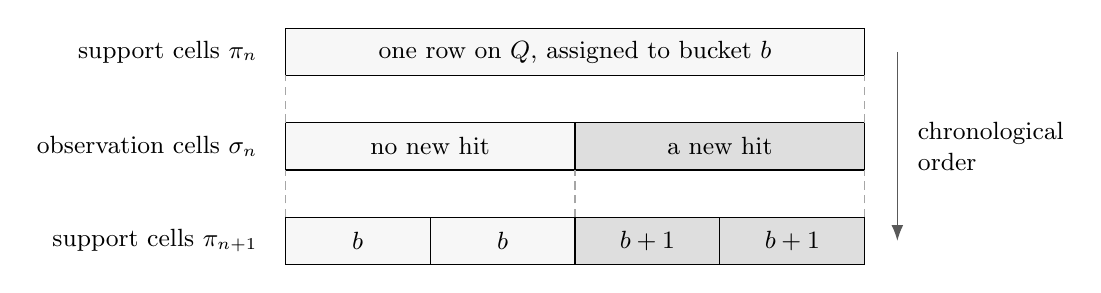
\begin{tikzpicture}[x=0.92cm,y=1cm,box/.style={draw,minimum height=6mm},every node/.style={font=\small}]
  \node[anchor=east] at (-0.25,2.7) {support cells $\pi_n$};
  \node[anchor=east] at (-0.25,1.5) {observation cells $\sigma_n$};
  \node[anchor=east] at (-0.25,0.3) {support cells $\pi_{n+1}$};

  \draw[fill=black!3] (0,2.4) rectangle (8,3.0);
  \node at (4,2.7) {one row on $Q$, assigned to bucket $b$};

  \draw[fill=black!3] (0,1.2) rectangle (4,1.8);
  \draw[fill=black!13] (4,1.2) rectangle (8,1.8);
  \node at (2,1.5) {no new hit};
  \node at (6,1.5) {a new hit};

  \draw[fill=black!3] (0,0) rectangle (2,0.6);
  \draw[fill=black!3] (2,0) rectangle (4,0.6);
  \draw[fill=black!13] (4,0) rectangle (6,0.6);
  \draw[fill=black!13] (6,0) rectangle (8,0.6);
  \node at (1,0.3) {$b$};
  \node at (3,0.3) {$b$};
  \node at (5,0.3) {$b+1$};
  \node at (7,0.3) {$b+1$};

  \draw[densely dashed,black!35] (0,0.6)--(0,1.2) (4,0.6)--(4,1.2) (8,0.6)--(8,1.2);
  \draw[densely dashed,black!35] (0,1.8)--(0,2.4) (8,1.8)--(8,2.4);
  \draw[-{Latex[length=2mm]},black!65] (8.45,2.7)--(8.45,0.3);
  \node[anchor=west,align=left] at (8.6,1.5) {chronological\\order};
\end{tikzpicture}

\caption{Schematic view of one branch of the spatial partitions in consecutive
rounds.  The row on $Q$ has already entered bucket $b$ before a new hit is tested.
Hits may differ on the observation cells.  Each support cell in the next
round lies inside one observation cell, so every row in that round still
receives one bucket; the bottom labels give those bucket numbers.}
\label{fig:row-chronology}
\end{figure}

Let $\mathcal B_i$ be the rows assigned to bucket $i$, and set
\[
 v_i=\sum_{\nu\in\mathcal B_i} A_\nu^*c_\nu,\qquad 1\le i\le T.
\]
For every subset $J\subset\{1,\ldots,T\}$, the adjoint of the
joint operator in the hypothesis gives
\begin{equation}
 \left\|\sum_{i\in J}v_i\right\|_2^2
 \le B^2\sum_{\nu\in\bigcup_{i\in J}\mathcal B_i}
                   \|c_\nu\|_{\mathcal Y_\nu}^2.
 \label{eq:row-bucket-bessel}
\end{equation}
Although the sets $\mathcal B_i$ depend on the fixed test vector,
they are actual subsets of the original row indices.  Thus
Equation~\eqref{eq:row-bucket-bessel} is the original operator
inequality applied to a test vector with some coordinates set to
zero.  In particular
\[
 \sum_{i=1}^T\|v_i\|_2^2\le B^2E_c.
\]

Let $\Omega_T$ be the set of points whose path has $T$ hits during
these rounds.  At any point $y$, a tested adjoint from $\mathcal B_i$
whose support does not contain $y$ vanishes there.  If its support
contains $y$, it was assigned $i$ exactly when the path's current
bucket was $i$; conversely, before stopping, every tested adjoint
whose support contains $y$ enters that current bucket.
Thus, on $\Omega_T$, $v_i(y)$ is exactly the sum accumulated in
bucket $i$ up to and including the round that causes its hit.
The coefficient vector of this sum has norm greater than $\tau$.  All its labels remain
available on the final observation cell containing $y$, so
Equation~\eqref{eq:row-catalog-comparison} yields
$\|v_i(y)\|_{\mathcal H}>D^{-1}\tau$ for $1\le i\le T$.
Consequently
\begin{equation}
 |\Omega_T|
 \le \frac{B^2E_c}{TD^{-2}\tau^2}
 =\frac{16D^5B^2E_c}{T\lambda^2}.
 \label{eq:row-many-hits}
\end{equation}

Outside $\Omega_T$, at any intermediate round the partial sum
equals a prefix of the completed bucket sums $v_i(y)$ plus the
current unfinished sum.  The latter has coefficient norm at most
$\tau$, and hence has Hilbert norm at most
$D^{3/2}\tau=\lambda/4$.  This statement also includes the instant
of a hit, by putting the newly completed bucket in the prefix and
taking unfinished sum zero.  Thus, with
\[
 M_T(y)=\max_{0\le j\le T}\left\|\sum_{i=1}^jv_i(y)\right\|_{\mathcal H},
\]
one has
\begin{equation}
 M(y)\le M_T(y)+\lambda/4\qquad(y\notin\Omega_T)
 \label{eq:row-prefix-domination}
\end{equation}
outside the fixed null set.

It remains to estimate $M_T$ using
Equation~\eqref{eq:row-bucket-bessel}.  We use the binary-prefix argument
of Rademacher--Menshov type; compare \cite[Lemma~2.7]{KrauseLacey2020}.
For each
$0\le k\le\log_2T$, let $\mathcal D_k$ be the partition of
$\{1,\ldots,T\}$ into consecutive dyadic index intervals of length
$2^k$, and put $v_J=\sum_{i\in J}v_i$.  Every prefix is the disjoint
union of at most one interval from each $\mathcal D_k$.  The triangle
inequality therefore gives pointwise
\[
 M_T\le
 \sum_{k=0}^{\log_2T}
       \left(\sum_{J\in\mathcal D_k}\|v_J\|_{\mathcal H}^2\right)^{1/2}.
\]
For a fixed $k$, Equation~\eqref{eq:row-bucket-bessel} and the
disjointness of the index intervals imply
\[
 \int_R\sum_{J\in\mathcal D_k}\|v_J(y)\|_{\mathcal H}^2\,dy
 =\sum_{J\in\mathcal D_k}\|v_J\|_2^2
 \le B^2E_c.
\]
Minkowski's inequality in $L^2(R)$ now gives
\begin{equation}
 \|M_T\|_2\le (1+\log_2T)B E_c^{1/2}=L_D B E_c^{1/2}.
 \label{eq:row-binary-prefix}
\end{equation}

Equations~\eqref{eq:row-many-hits}--\eqref{eq:row-binary-prefix}
and Chebyshev's inequality show that
\[
 \begin{split}
 |\{M>\lambda\}|
 &\le |\Omega_T|+|\{M_T>3\lambda/4\}|\\
 &\le \frac{16B^2E_c}{\lambda^2}
             \left(\frac{D^5}{T}+\frac{L_D^2}{9}\right)
 \le \frac{16(9+L_D^2)B^2E_c}{9\lambda^2},
 \end{split}
\]
because $T\ge D^5$.  This is the stated weak estimate, as
$\mathfrak C_D^2/4=16(9+L_D^2)/9$.  Integrating the minimum of
this estimate and $|R|$ over $\lambda>0$ proves the $L^1$ estimate:
for $H=(\mathfrak C_D/2)BE_c^{1/2}>0$,
\[
 \int_0^\infty\min\{|R|,H^2/\lambda^2\}\,d\lambda
 =2H|R|^{1/2}.
\]
If $H=0$, the weak estimate gives $M=0$ almost everywhere instead.
Finally, put $x=\log_2D\ge1$.  Since $L_D\le5x+2$ and
$9+(5x+2)^2\le25(x+1)^2$, the asserted upper bound on
$\mathfrak C_D$ follows.
\end{proof}

\begin{lemma}[The depth-varying row estimate]
\label{lem:row-depth}
Let the root, catalog, partitions, and rows satisfy every hypothesis
of Lemma~\ref{lem:row-maximal}.  Let $(F_s)_{s\in\mathsf S}$ satisfy
Equation~\eqref{eq:row-input-normalization} on $R$.  Choose
$s_n\in\mathsf S$ with
$s_1\le s_2\le\cdots\le s_N$, and let every row of round $n$
read the same input $F_{s_n}$.  These read indices label the input
schedule independently of the spatial depths of the support cells.  Then
\begin{equation}
 \left(\sum_{n=1}^N\sum_{\nu\in\mathcal R_n}
          \|A_\nu F_{s_n}\|_{\mathcal Y_\nu}^2\right)^{1/2}
 \le \mathfrak C_D B\,|R|^{1/2}
 \le \frac{40}{3} B\log_2(2D)\,|R|^{1/2}.
 \label{eq:row-depth}
\end{equation}
The constant is independent of the number of rows, depths, and
input blocks.
\end{lemma}

\begin{proof}
Test the output vector against arbitrary
$c=(c_\nu)_{\nu\in\mathcal R}$ in the finite Hilbert direct sum of
the row spaces.  The rounds whose read index lies in a particular
block $\mathsf S_b$ are consecutive, or absent, because the
$s_n$ are nondecreasing.  On a nonempty such range $p\le n\le q$,
form $g_n,S_n,M$ as in Lemma~\ref{lem:row-maximal}.  Pointwise Abel
summation, with the stipulated inner-product convention, is
\[
 \sum_{n=p}^q\langle F_{s_n},g_n\rangle_{\mathcal H}
 =\langle F_{s_q},S_q\rangle_{\mathcal H}
   +\sum_{n=p}^{q-1}
       \langle F_{s_n}-F_{s_{n+1}},S_n\rangle_{\mathcal H}.
\]
The absolute value of this expression is at most
\[
 \left(\|F_{s_q}\|_{\mathcal H}
       +\sum_{n=p}^{q-1}\|F_{s_{n+1}}-F_{s_n}\|_{\mathcal H}\right)M
 \le W^{-1/2}M.
\]
For the last inequality, the nondecreasing reads traverse each
edge in the block at most once; repeated reads contribute zero.
Integrating and using Equation~\eqref{eq:row-maximal} bounds this
block's pairing by
\[
 \mathfrak C_D B\,W^{-1/2}|R|^{1/2}
       \left(\sum_{n=p}^q\sum_{\nu\in\mathcal R_n}
                         \|c_\nu\|_{\mathcal Y_\nu}^2\right)^{1/2}.
\]
All sums are finite and each pairing is integrable by the $L^2$
inequality, so the pointwise identity may be integrated.  Write
$E_b$ for the squared coefficient sum in the last display, with
$E_b=0$ for an absent block.  The adjoint identity and
Cauchy--Schwarz over the $W$ blocks give
\[
 \begin{split}
 \left|\sum_{n=1}^N\sum_{\nu\in\mathcal R_n}
              \langle A_\nu F_{s_n},c_\nu\rangle_{\mathcal Y_\nu}\right|
 &\le \mathfrak C_D B\,|R|^{1/2}
                  W^{-1/2}\sum_{b=1}^W E_b^{1/2}\\
 &\le \mathfrak C_D B\,|R|^{1/2}
        \left(\sum_{\nu\in\mathcal R}\|c_\nu\|_{\mathcal Y_\nu}^2\right)^{1/2}.
 \end{split}
\]
Duality in the finite Hilbert direct sum proves
Equation~\eqref{eq:row-depth}.
\end{proof}

The realized finite rows, partitions, and catalog may depend on the given
depth inputs, provided they satisfy all preceding hypotheses and are held
fixed while their ordinary operator inequality is tested on arbitrary inputs.

\subsection{Projection increments}

Here is a useful consequence for the inherited local projections
of H.  It also records why their splitting into support cells
preserves the original Bessel bound.

\begin{corollary}[Increments of inherited projections]
\label{cor:row-projections}
Use the catalog of Lemma~\ref{lem:row-catalog}.  On a finite
interval of integers $h\ge s_R$, let $\mathcal P_h$ be the full
partition of $R$ into cells of depth $h$.  On each
$Q\in\mathcal P_h$, let $P_{h,Q}$ be the orthogonal projection in
$L^2(Q;\mathcal H)$ onto constant-coefficient combinations of
a subset $\mathcal M_h(Q)\subset\mathcal V(Q)$.  Assume inheritance:
if $Q'\in\mathcal P_{h+1}$ is contained in $Q$, then
$\mathcal M_h(Q)\subset\mathcal M_{h+1}(Q')$.  Let $P_h$ be the
direct sum of the $P_{h,Q}$ on $L^2(R;\mathcal H)$.

Suppose $(F_s)_{s\in\mathsf S}$ satisfies
Equation~\eqref{eq:row-input-normalization}.  For any integer $J\ge1$ and
\[
 r_1\le t_1\le r_2\le t_2\le\cdots\le r_J\le t_J
\]
in the projection depth range and nondecreasing
$s_1,\ldots,s_J\in\mathsf S$, one has
\begin{equation}
 \sum_{j=1}^J\|(P_{t_j}-P_{r_j})F_{s_j}\|_2^2
 \le \mathfrak C_D^2|R|.
 \label{eq:row-disjoint-increments}
\end{equation}
If the intervals can be divided into $\mathfrak m$ such ordered
families whose reads are nondecreasing, the right side is multiplied
by $\mathfrak m$.

For each $s\in\mathsf S$ with $s\ge s_R$, let $\mathcal U_s$ be any
subcollection of the depth-$s$ cells of $R$.  In particular fix an integer
$\ell$ and retain only those $s$ for which $s+\ell$ and $s+\ell+1$ are in
the projection range.  Then
\begin{equation}
 \sum_s\sum_{I\in\mathcal U_s}|I|\,
       \|(P_{s+\ell+1}-P_{s+\ell})F_s\|_{2,I}^2
 \le \mathfrak C_D^2|R|.
 \label{eq:row-increment}
\end{equation}
For every integer $L\ge0$, retaining only $s\in\mathsf S$ with $s\ge s_R$
for which $s$ and $s+L$ are in the projection range,
\begin{equation}
 \left(\sum_s\sum_{I\in\mathcal U_s}|I|\,
       \|(P_{s+L}-P_s)F_s\|_{2,I}^2\right)^{1/2}
 \le L\mathfrak C_D|R|^{1/2}
 \le (1+L)\mathfrak C_D|R|^{1/2}.
 \label{eq:row-delay}
\end{equation}
\end{corollary}

\begin{proof}
The range of $P_h$ is contained in the range of $P_{h+1}$:
restrict a constant-coefficient combination on $Q$ to its
children and use inheritance.  Thus the $P_h$ are nested
orthogonal projections.  For $r\le t$, $P_t-P_r$ is an
orthogonal projection, and the projections corresponding to
intervals with disjoint interiors have pairwise orthogonal ranges.

For a cell $Q\in\mathcal P_r$, both $P_r$ and $P_t$ commute with
multiplication by $\mathbf1_Q$, since both of their defining
partitions refine $\mathcal P_r$.  The row
\[
 A_{j,Q}=(P_{t_j}-P_{r_j})\mathbf1_Q:
        L^2(R;\mathcal H)\longrightarrow L^2(R;\mathcal H),
 \qquad Q\in\mathcal P_{r_j},
\]
has both input and output supported in $Q$.  Consequently
\[
 \sum_{Q\in\mathcal P_{r_j}}\|A_{j,Q}z\|_2^2
 =\|(P_{t_j}-P_{r_j})z\|_2^2,
 \qquad
 \sum_{j,Q}\|A_{j,Q}z\|_2^2\le\|z\|_2^2.
\]
This establishes the joint Bessel bound after the splitting.
The adjoint of $A_{j,Q}$ is
$\mathbf1_Q(P_{t_j}-P_{r_j})$.  On a cell of
$\mathcal P_{t_j}$ its first term is a constant-coefficient
combination there, while its second term is the restriction of
such a combination on an $r_j$-cell.  Both use labels available
on the $t_j$-cell.  Therefore the support and observation
partitions in Lemma~\ref{lem:row-depth} are
$\mathcal P_{r_j}$ and $\mathcal P_{t_j}$, respectively.
The stated order of intervals gives the required refinement,
and Lemma~\ref{lem:row-depth} with $B=1$ proves
Equation~\eqref{eq:row-disjoint-increments}.  Summing the
estimates for $\mathfrak m$ subfamilies proves the overlap version.
After discarding the zero increments $r=t$, intervals with edge overlap
$\mathfrak m$ can be so divided by the usual greedy coloring in increasing left
endpoint, whenever the reads in that order are nondecreasing:
at a left endpoint fewer than $\mathfrak m$ colors are occupied
by earlier intervals whose right endpoints are still larger.

For fixed $\ell$, the intervals $[s+\ell,s+\ell+1]$ are
consecutive and their reads $s$ increase.  Apply
Equation~\eqref{eq:row-disjoint-increments}.  At each $s$ the
cells in $\mathcal U_s$ are disjoint, and
$|I|\|z\|_{2,I}^2=\|\mathbf1_Iz\|_2^2$.  Restricting the
outputs to those cells can only decrease their squared sum,
which proves Equation~\eqref{eq:row-increment}.  Finally,
\[
 (P_{s+L}-P_s)F_s
 =\sum_{\ell=0}^{L-1}(P_{s+\ell+1}-P_{s+\ell})F_s.
\]
Minkowski's inequality in the Hilbert direct sum over $(s,I)$
and Equation~\eqref{eq:row-increment} prove
Equation~\eqref{eq:row-delay}.  For $L=0$ both sides of its
first inequality are zero.
\end{proof}

\subsection{Smooth rows with fixed carriers}

The remaining rows have smooth mean-zero test functions on their
support cells, multiplied by a fixed function that may oscillate
arbitrarily.  Dyadic differences make their coefficients constant
on finer cells.  Private coordinates can then be adjoined at a
controlled cost.

\begin{lemma}[Smooth mean-zero rows on depth inputs]
\label{lem:smooth-depth}
Let $R$ be a finite dyadic root and let $\mathcal N$ be a finite
set of carrier labels.  For each $\nu\in\mathcal N$ fix one
measurable function $m_\nu:R\to\mathbb C$ with
$\|m_\nu\|_\infty\le1$.  This function is the same for every
interval using the label $\nu$.  Let $\mathcal E$ be a finite
set of pairs $(I,\nu)$, where $I\subset R$ is a dyadic interval
of depth $s(I)$ and $\nu\in\mathcal N$.  Thus at most one row
is selected for a given pair $(I,\nu)$.

For each selected pair, let $\omega_{I,\nu}\in C^1(\overline I)$
satisfy
\[
 \int_I\omega_{I,\nu}(y)\,dy=0,\qquad
 \|\omega_{I,\nu}\|_\infty+
       |I|\|\omega_{I,\nu}'\|_\infty\le A
\]
for one $A\ge0$.  Suppose the selected physical rows
\[
 \mathcal W_{I,\nu}f
   =|I|^{-1/2}\int_I m_\nu(y)\omega_{I,\nu}(y)f(y)\,dy
\]
satisfy, for one $B_H\ge0$,
\[
 \sum_{(I,\nu)\in\mathcal E}|\mathcal W_{I,\nu}f|^2
 \le B_H^2\|f\|_{L^2(R)}^2\qquad(f\in L^2(R)).
\]
Let the scalar functions $(f_s)_{s\in\mathsf S}$ satisfy
Equation~\eqref{eq:row-input-normalization}, with absolute
values in place of Hilbert norms, and assume that every
$s(I)$ belongs to $\mathsf S$.  Put
\[
 d=2+\#\mathcal N,\qquad h_0=\lceil10\log_2(2d)\rceil.
\]
Then
\begin{equation}
 \begin{split}
 \left(\sum_{(I,\nu)\in\mathcal E}
           |\mathcal W_{I,\nu}f_{s(I)}|^2\right)^{1/2}
 &\le \mathfrak C_d\left[
       (h_0+1)(B_H+3A)
       +2A\sqrt d\,(h_0+3)2^{-h_0}\right]|R|^{1/2}\\
 &\le 760(B_H+A)\bigl(\log_2(2d)\bigr)^2|R|^{1/2}.
 \end{split}
 \label{eq:smooth-depth}
\end{equation}
The estimate uses only the displayed Bessel inequality for the
selected set $\mathcal E$, not for any larger array of intervals
and carriers.
\end{lemma}

\begin{proof}
The assertion is immediate if $\mathcal E$ is empty.  Extend each
$\omega_{I,\nu}$ by zero off $I$.  Let $\mathbb E_h$ be dyadic
conditional expectation on the full depth-$h$ partition of $R$;
we use it for every integer $h\ge s_R$.  These are nested orthogonal
projections in $L^2(R)$.  For $s=s(I)$, exact mean zero and the zero
extension give $\mathbb E_s\overline{\omega_{I,\nu}}=0$.  Define the
difference pieces for $h\ge1$ and the initial sum by
\[
 \begin{aligned}
 q_{I,\nu,h}
 &=|I|^{-1/2}(\mathbb E_{s+h}-\mathbb E_{s+h-1})
                         \overline{\omega_{I,\nu}}\quad(h\ge1),\\
 q_{I,\nu,0}
 &=|I|^{-1/2}\mathbb E_{s+h_0}\overline{\omega_{I,\nu}}
 =\sum_{h=1}^{h_0}q_{I,\nu,h}.
 \end{aligned}
\]
Every $q_{I,\nu,h}$ is supported in $I$, and for $h\ge1$ it
is constant on depth-$(s+h)$ cells and lies in the martingale
difference space
$\operatorname{range}(\mathbb E_{s+h}-\mathbb E_{s+h-1})$.
The initial sum is constant on depth-$(s+h_0)$ cells.
The zero extension causes no difficulty: cells at these depths
do not cross the boundary of $I$.

On a child of a depth-$(s+h-1)$ cell, the difference between
its average of $\omega_{I,\nu}$ and the parent's average is
at most the oscillation on the parent.  The derivative bound
therefore gives
\begin{equation}
 \|q_{I,\nu,h}\|_2\le 2A\,2^{-h}\qquad(h\ge1).
 \label{eq:smooth-difference-size}
\end{equation}
For a fixed $\nu$ and $h$, these functions are pairwise
orthogonal as $I$ varies through the selected pairs.  Indeed,
different support depths give different martingale difference
spaces.  At one depth the distinct intervals are disjoint,
and there is at most one selected row for $(I,\nu)$.
Thus their analysis operator has norm at most $2A2^{-h}$.
Since multiplication by the one fixed $m_\nu$ is a contraction,
the physical lag-$h$ rows, whose adjoints are
$q_{I,\nu,h}\overline{m_\nu}$, have joint operator norm at most
\begin{equation}
 B_{\mathrm{phys},h}\le 2A\sqrt{\#\mathcal N}\,2^{-h}
 \le 2A\sqrt d\,2^{-h}.
 \label{eq:smooth-physical-lag}
\end{equation}
This argument uses the fixedness and boundedness of $m_\nu$,
and requires no regularity or frequency separation for it.

The derivative bound implies uniform convergence on $I$
of $\mathbb E_{s+H}\omega_{I,\nu}$ to $\omega_{I,\nu}$ as
$H\to\infty$.  Consequently
\[
 |I|^{-1/2}\overline{\omega_{I,\nu}}
 =q_{I,\nu,0}+\sum_{h>h_0}q_{I,\nu,h}.
\]
The associated physical row series also converges in operator norm,
by Equation~\eqref{eq:smooth-physical-lag}.
Subtracting its tail from the original selected row operator
therefore proves
\[
 B_{\mathrm{phys},0}
 \le B_H+2A\sqrt{\#\mathcal N}\,2^{-h_0}
 \le B_H+A.
\]
For the last inequality use
$2^{-h_0}\le(2d)^{-10}$ and $d\ge2$.

Adjoin one private direction for each complete carrier.
Specifically take
$\mathcal H^{\mathrm{aug}}=\mathbb C\oplus\ell^2(\mathcal N)$
and the root-born columns
\[
 \Phi_\nu(y)=(\overline{m_\nu(y)},\mathbf e_\nu),\qquad y\in R.
\]
Their norms are at most $\sqrt2$, their private constants have
size one, and the number of labels on any path is
$\#\mathcal N\le d$.  They satisfy
Equation~\eqref{eq:row-catalog-budget} with $D=d$.
For $h=0$ and for $h>h_0$, define the augmented scalar row by
\[
\widetilde{\mathcal W}_{I,\nu,h}Z
 =\langle Z,q_{I,\nu,h}\Phi_\nu\rangle_{L^2(R;\mathcal H^{\mathrm{aug}})}.
\]
Write $\widetilde{\mathcal W}_h$ for the joint operator consisting
of these rows over $(I,\nu)\in\mathcal E$.
The adjoint of the individual row sends $c$ to
$c\,q_{I,\nu,h}\Phi_\nu$.  On a physical input $Z=(f,0)$,
\[
 \widetilde{\mathcal W}_{I,\nu,h}(f,0)
 =\langle m_\nu f,q_{I,\nu,h}\rangle_{L^2(R)},
\]
which is exactly the physical row for the corresponding bump piece.

For a private input $z=(z_\nu)_{\nu\in\mathcal N}$, the lag-$h$
analysis map has entries $\langle z_\nu,q_{I,\nu,h}\rangle$.
The fixed-$\nu$ orthogonality already proved, followed by
orthogonality of the private coordinates, gives its norm at
most $2A2^{-h}$.  The physical and private input summands are
orthogonal.  Applying Cauchy--Schwarz to their two norm bounds
and using Equation~\eqref{eq:smooth-physical-lag} gives
\begin{equation}
 \|\widetilde{\mathcal W}_h\|
 \le 2A\sqrt{\#\mathcal N+1}\,2^{-h}
 \le 2A\sqrt d\,2^{-h}\qquad(h>h_0).
 \label{eq:smooth-augmented-lag}
\end{equation}
For the initial sum, the identity
$q_{I,\nu,0}=\sum_{h=1}^{h_0}q_{I,\nu,h}$ and the operator
triangle inequality bound its private part by
$2A\sum_{h=1}^{h_0}2^{-h}\le2A$.  Its physical part has the
bound $B_H+A$ above.  Thus
\begin{equation}
 \|\widetilde{\mathcal W}_0\|\le B_H+3A.
 \label{eq:smooth-augmented-main}
\end{equation}

The two pieces, each indexed by the same selected set $\mathcal E$, have
the following data:
\begin{center}
\small
\begin{tabular}{@{}lccc@{}}
\hline
Piece & Observation depth & \shortstack{Joint augmented\\operator norm}
& \shortstack{Residue modulus\\for support depths}\\
\hline
Initial sum $q_0$ & $s+h_0$ & $B_H+3A$ & $h_0+1$\\
Lag $q_h$, $h>h_0$ & $s+h$ & $2A\sqrt d\,2^{-h}$ & $h+1$\\
\hline
\end{tabular}
\end{center}
For either piece, let $\ell$ denote its observation offset, namely $h_0$
or $h$.  Each row is supported on its whole cell $I$ of depth $s=s(I)$,
and its adjoint coefficient is constant on depth-$(s+\ell)$ cells.
Divide the selected support depths into residue classes modulo $\ell+1$.
Within one class, group all selected rows of one depth $s$ in one round,
using the full depth-$s$ support partition and the full depth-$(s+\ell)$
observation partition of $R$; unused cells carry no rows.  Successive
support depths differ by at least $\ell+1$, so the next support partition
refines the preceding observation partition.  All rows in a round read
the same $F_s=(f_s,0)$, and these indices increase in $\mathsf S$.
The catalog has $D=d$, and restricting either displayed array to a
residue class preserves its operator bound.  Lemma~\ref{lem:row-depth}
therefore applies in each of the at most $\ell+1$ classes.

Write $V_0\in\ell^2(\mathcal E)$ for the outputs of the initial sum on
their respective $F_{s(I)}$, and $V_h\in\ell^2(\mathcal E)$ for the
analogous lag-$h$ vector.  Extending each residue-class vector by zero
to the full selected row space and using its triangle inequality yields
\[
 \|V_0\|_{\ell^2(\mathcal E)}
 \le (h_0+1)\mathfrak C_d(B_H+3A)|R|^{1/2},
 \qquad
 \|V_h\|_{\ell^2(\mathcal E)}
 \le (h+1)\mathfrak C_d\,2A\sqrt d\,2^{-h}|R|^{1/2}.
\]
These bounds are summable over $h>h_0$.  The uniform bump
expansion gives rowwise
$\mathcal W_{I,\nu}f_{s(I)}
= (V_0)_{I,\nu}+\sum_{h>h_0}(V_h)_{I,\nu}$.
There are finitely many selected rows; alternatively the last
summable bounds give convergence directly in their Hilbert
sum.  Minkowski's inequality and
\[
 \sum_{h>h_0}(h+1)2^{-h}=(h_0+3)2^{-h_0}
\]
prove the first inequality in Equation~\eqref{eq:smooth-depth}.
For its last inequality put $l=\log_2(2d)\ge2$.  Then
$h_0+1\le11l$, $h_0+3\le12l$, and
$\sqrt d\,2^{-h_0}\le1$.  The bracket there is at most
$57(B_H+A)l$, while
$\mathfrak C_d\le(40/3)l$.  Their product is at most
$760(B_H+A)l^2$, as asserted.
\end{proof}

\section{The base reduction with varying depth inputs}
\label{sec:base}

We prove Theorem~\ref{thm:depth-local} by adapting the local-form
construction of \cite[Sections~3--10]{H}.  The scalar analytic and
finite combinatorial estimates remain those of H.  The row estimates
of Section~\ref{sec:rows} replace the uses of one original input at
different depths.  This section constructs the tuple to which the
later localization applies: cyclic approximations first give a tuple
\(X\), delayed high fits replace it by \(Y\), and the decomposition
\(Y=B+U\) leaves three active patterns.

Fix the root \(J\), finite tree \(\mathcal T\), original summation
collection \(\mathcal I\), and four input schedules of
Theorem~\ref{thm:depth-local}.  Write
\(s(I)=\log_2(|J|/|I|)\).  On every subroot \(R\), the spatial origin
\(s_R\) of Section~\ref{sec:rows} is \(s(R)\); a restart does not reset
depth.  The actual augmented input is \(F_{j,s}=(f_{j,s},0)\).
Finitely needed temporal indices beyond the schedule use its nearest
endpoint value, while the spatial inputs remain zero outside \(J\).
In the local forms put \(y_j=x+jt\), \(0\le j\le3\), and use the
normalized norms of Definition~\ref{def:transfer-local-kernels}.
Only physical components enter a form.  The notation \(\Heq{n}\)
denotes Equation~\((n)\) of H.

Fix provisionally one \(q\) with \(2<q<3\).  Section~\ref{sec:completion}
will choose a single value satisfying both arguments' degree restrictions
and run H's fixed-input proof at that exponent.  Polynomial degrees below are
absolute; their coefficients and the lower accuracy threshold may
depend on \(q,c_0,C_0\).  Accuracy indices \(t\) are independent of
spatial depths \(s,h\).

\subsection{Inputs, source columns, and the row estimate}

Lemma~\ref{lem:depth-input-size} and Equation~\eqref{eq:row-variation}
give, on every subroot \(R\subseteq J\),
\begin{gather}
 \|F_{j,s}\|_{p,I}\le1,\qquad
 \|\mathbf1_R F_{j,s}\|_2\le |R|^{1/2}
 \quad(1\le p\le\infty),                                      \label{eq:h-input-size}\\
 \sum_{[r,t]}\|\mathbf1_R(F_{j,t}-F_{j,r})\|_2^2
       \le5a|R|.                                               \label{eq:h-input-variation}
\end{gather}
The first bound holds on every descendant \(I\) and every prescribed
or finitely extended input index.  The second holds for depth intervals
with edge overlap at most \(a\).  Restriction to a subroot, a
nondecreasing subsequence, and repeated reads preserve these
conclusions.  Each slot retains its own full block schedule.  We also
use the \emph{Local absolute estimate} Lemma of \cite[Section~2]{H}:
\[
 |H_I(z_0,z_1,z_2,z_3)|
 \le C\prod_{j=0}^3\|z_j\|_{p_j,I},
 \qquad p_j\ge1,\quad \sum_jp_j^{-1}\le2.
\]

The scalar labels are restrictions to their birth cells of the
bounded quadratic chart atoms in the \emph{Quadratic chart atom}
Definition of \cite[Section~4]{H}.  We use exactly that
source-defined class and complexity: \(H\ge e^2\) bounds the chart
dimension by \(\log H\), the rational matrix height and amplitude
support by \(H\), and the amplitude derivatives by the fixed
bounds in that Definition.  The real quadratic, linear, and
horizontal oscillation parameters are unrestricted.  A bounded
atom has supremum norm at most one, with scalar normalization
factors kept in the external coefficients.  The
\emph{Elementary chart operations} Lemma of \cite[Section~4]{H}
permits conjugation, bounded products, and affine changes of the
real argument with a quasipolynomial complexity change.  We write
\(e(v)=\exp(2\pi i v)\).

For a birth label \(v\), write
\(\Phi_v=(\varphi_v,\sqrt{\epsilon_v}\mathbf e_v)\), with the
persistent birth cell and distinct private direction of
Section~\ref{sec:rows}.  A joint budget \(D\ge2\) means exactly
Equation~\eqref{eq:row-catalog-budget}, including every available
label on a path.  Lemma~\ref{lem:row-catalog}, equivalently the
\emph{Coefficient and projection bounds} Lemma of
\cite[Section~3]{H}, gives for constant coefficients on a cell \(I\)
where the labels are available
\begin{equation}
 D^{-1}\|c\|_{\ell^2}\le
 \left\|\sum_v c_v\Phi_v(y)\right\|
 \le D^{3/2}\|c\|_{\ell^2}
 \quad\text{for almost every }y\in I.                         \label{eq:h-column-bounds}
\end{equation}
Let \(P_{I,\mathcal V}\) denote the local orthogonal projection onto
the constant-coefficient span of an available mask \(\mathcal V\).
The same source Lemma gives
\[
 \|P_{I,\mathcal V}z\|_{\infty,I}\le D^5\fint_I\|z\|,
 \qquad
 \fint_I\bigl(f-(P_{I,\mathcal V}(f,0))_{\rm phys}\bigr)
       \overline{\varphi_v}=\epsilon_v c_v,
\]
where \(c_v\) is that projection's coefficient.  Inherited masks
retain their admitted labels on children; their full-partition direct
sums are nested orthogonal projections.  At a summation cut, the
continuation convention of \cite[Section~3]{H} retains the old labels
and locally refits them on every finer cell needed for the old
summands.  A new attempt may use a separate family.  On a subroot,
Lemma~\ref{lem:row-catalog} rebases inherited labels without changing
their private constants.  These are local refits of the retained
spans.

For every fixed realized finite row array and catalog satisfying
Lemma~\ref{lem:row-depth}, with ordinary Bessel norm \(B\), that Lemma
gives
\begin{equation}
 \sum_\nu\|B_\nu F_{j,s(\nu)}\|^2
 \le C B^2\log^2(2D)|R|.                                     \label{eq:h-row-use}
\end{equation}
The read \(s(\nu)\) is common to its round and nondecreasing between
rounds.  The realized rows and catalog may have been selected using
the schedules; they are fixed while the ordinary operator inequality
is tested on arbitrary inputs.

\subsection{One capped trial and cyclic adaptive fits}

For a physical residual \(r\) in slot \(j\), let
\(\mathfrak d_{j,I}(r)\) be the supremum of the form against two
normalized \(L^2(I)\) inputs and one normalized \(L^q(I)\) input in
the other slots, with the \(L^q\) slot arbitrary.  The
\emph{Local detection} Lemma of \cite[Section~4]{H} says that if
\(C_1\ge1\), \(0<\delta<1/2\), \(\|r\|_{2,I}\le C_1\), and
\(\mathfrak d_{j,I}(r)>\delta\), there is a bounded chart atom
\(\varphi\) such that
\[
 \left|\fint_I r\overline\varphi\right|\ge\rho,\qquad
 \log(1/\rho),\ \log(\operatorname{complexity}(\varphi))
 \le C_q\bigl(1+\log C_1+\log(1/\delta)\bigr)^C.
\]
We may decrease \(\rho\) to lie in \((0,1]\).  The form norm of two
specified factors below is the supremum against two normalized
\(L^2(I)\) inputs in their complementary slots.

\begin{lemma}[One capped insertion trial]
\label{lem:hbase-trial}
Let \(R\) be an attempt root with a restricted normalized input
schedule \(F_s\).  Let the candidate request cells belong to a fixed finite
original request tree below \(R\).  Fix
\(0<\rho\le1\), \(D_0\ge2\), and an integer cap \(T\ge1\).
Process candidates in nondecreasing request-cell depth, allowing
repetitions at one cell.  Stop before the first request that would
exceed \(T\) successful requests on its spatial path, and remove
that cut cell and its candidate descendants from the trial.

For each successful request \(v\) at \(I_v\), suppose there is a
set \(\mathcal R_v\) of charged row indices, with these sets pairwise
disjoint, such that
\[
 \sum_{\nu\in\mathcal R_v}
       \|\Delta_\nu F_{s(\nu)}\|_2^2
 \ge c\rho^2|I_v|.
\]
Assume all charged rows are a Bessel-norm-one subfamily of one
realized finite nested sequence of full-partition projections and
satisfy every hypothesis of Lemma~\ref{lem:row-depth}.  Suppose its
completed catalog has budget
\[
 D_T\le C D_0(T+1)^C,
\]
where \(D_0\) includes all predetermined columns, including their
future admissions on this attempt.  Then the disjoint first-excess
cells \(\mathcal C_T\), which are original request-tree cells, obey
\begin{equation}
 \sum_{I\in\mathcal C_T}|I|
 \le C T^{-1}\rho^{-2}\log^2(2D_T)|R|.                        \label{eq:hbase-trial-cut}
\end{equation}
If
\[
 a=1+\log(2D_0)+\log(1/\rho),\qquad
 T=\left\lceil C_*\rho^{-4}(1+a)^8\right\rceil,
\]
then a sufficiently large fixed \(C_*\) makes the right side at
most \(|R|/4\), and \(\log(2T)\le C(a+\log C_*)\).
\end{lemma}

\begin{proof}
Freeze the completed rows and catalog.  By their disjoint ownership
and Equation~\eqref{eq:h-row-use},
\[
 c\rho^2\sum_v|I_v|
 \le\sum_{\nu\ {\rm charged}}\|\Delta_\nu F_{s(\nu)}\|_2^2
 \le C\log^2(2D_T)|R|.
\]
Set \(n(y)=\#\{v:y\in I_v\}\).  Earlier request cells meeting a
candidate contain it or equal it, because request depths are
nondecreasing.  Thus their count is constant on that candidate.
Each first-excess cell lies in \(\{n\ge T\}\), and removing its
subtree makes these cells disjoint.  Tonelli's identity
\(\int_R n=\sum_v|I_v|\) proves
Equation~\eqref{eq:hbase-trial-cut}.

For the stated cap, the budget bound gives
\(\log(2D_T)\le C'(a+\log C_*)\).  Consequently the coefficient
in Equation~\eqref{eq:hbase-trial-cut} is at most
\[
 C C_*^{-1}\rho^2(1+a)^{-8}(a+\log C_*)^2,
\]
which is at most \(1/4\) for fixed sufficiently large \(C_*\).
The logarithmic cap bound follows from the same formula.
\end{proof}

We realize the Lemma's nested sequence in both applications by one
rule.  At each projection depth, refine and locally refit the entire
root partition, admit the predetermined columns prescribed there,
and then perform simultaneous insertion rounds.  Cells with no
request retain their projections.  The next depth refines the entire
partition, including branches with no later tests for this attempt.
Refinements, admissions, and identity transitions remain in the
nested sequence.  Splitting an insertion increment on all cells of
its partition preserves its joint Bessel norm, by the splitting
identity in Corollary~\ref{cor:row-projections}.  The following two
applications specify the charged supports, observations, and reads.

Apply this construction first to the
\emph{Inherited adaptive approximation} Lemma of
\cite[Section~5]{H}, at accuracy \(e^{-k}\), for the fixed provisional
\(q\) and sufficiently large \(k\).  Every attempt starts with an
empty fit catalog.  On an assigned original candidate cell \(I\) of
depth \(s\), test
\[
 r=f_{j,s}-(PF_{j,s})_{\rm phys},
\]
where \(P\) is the current local projection.  Contraction gives
\(\|r\|_{2,I}\le2\).  On failure of the \(\mathfrak d_{j,I}\)
test, Local detection supplies a bounded atom with moment \(\rho\),
where \(\log(1/\rho)\le k^{O(1)}\).  Adjoin
\((\varphi,\mathbf e_v)\) with a fresh private direction and refit.
For the new projection \(P^+\),
\begin{equation}
 \|(P^+-P)F_{j,s}\|_{L^2(I)}^2
 \ge
 \frac{\left|\int_I
  (f_{j,s}-(PF_{j,s})_{\rm phys})\overline\varphi\right|^2}
      {\|(\varphi,\mathbf e_v)\|_{L^2(I)}^2}
 \ge c\rho^2|I|.                                               \label{eq:hbase-fresh-gain}
\end{equation}
Indeed, projection of the fresh column off the old span preserves
its pairing with the old residual and can only reduce its norm.

Here each request owns its insertion row on \(I\).  The support and
observation partitions are the full depth-\(s\) partition, and every
round at this depth reads \(F_{j,s}\).  Their refinement and read
order therefore satisfy Lemma~\ref{lem:row-depth}.  The initial
budget \(D_0\) is fixed, and a path cap \(T\) adds at most \(T\)
bounded columns of private weight one, giving the required polynomial
budget \(D_T\).  Lemma~\ref{lem:hbase-trial} makes the cut cells have
total length at most one quarter of the attempt root.

On every child root the restricted schedule is still normalized;
the fit again starts with no columns and has the same detection,
gain, full-partition chronology, and budget.  The one-trial Lemma
therefore applies anew.  Its length bound prevents a child from
cutting itself, so all new roots are proper original request-tree
descendants.  The finite recursion terminates, and the attempt-root
lengths sum to at most
\(\sum_{n\ge0}4^{-n}|R|=4|R|/3\), as in H's packing argument.
Each original summand belongs to one attempt.  The old projection
family continues by inheritance and local refitting only for its
old summands and their operator estimates.

On a retained cell the fit has passed:
\[
 g_I=P_IF_{j,s},\qquad
 \mathfrak d_{j,I}\bigl(f_{j,s}-(g_I)_{\rm phys}\bigr)\le e^{-k},
 \qquad \|g_I\|_{2,I}\le1.
\]
Within a segment, masks are inherited.  The cap and Local detection
bound path counts and atom complexities by \(\exp(k^{O(1)})\).
Private weights are one, so the coefficient \(\ell^2\) norm is at
most the normalized projection norm; Cauchy--Schwarz over the path
labels gives the same \(\exp(k^{O(1)})\) physical supremum bound.
All these statements hold anew on a normalized subroot.

We now use these fits cyclically in all four slots.  Let
\(\iota(t)=(t-1)\bmod4\) be the slot updated at accuracy level \(t\).
Choose an absolute \(A>1\), a sufficiently large initial \(k_1\),
and set \(k_{t+1}=k_t^A\).  Write \(g_{t,I}=P^t_IF_{\iota(t),s}\)
for the fit at level \(t\), and set \(g_{t-4,I}=0\) before that
slot's first update.  For any fixed bounded number of levels,
intersect their segment families.  Every common root is a root of
one constituent family or the original root, so their total length
remains bounded.

\begin{lemma}[The two earliest increments on depth inputs]
\label{lem:hbase-X-output}
On each original summation cell \(I\), put \(s=s(I)\), its original
spatial depth in \(J\).  At a finite terminal level \(n\), write \(g_{e,n,I}\) for the last
fit in slot \(e\) at or before \(n\), or zero if there is none, and
put \(r_{e,n,I}=F_{e,s}-g_{e,n,I}\).  For \(u<t\) with
\(\iota(u)=i\ne j=\iota(t)\), let \(a,b\) be the other slots and set
\begin{equation}
 \begin{aligned}
 X_i^{u,t}&=g_{u,I}-g_{u-4,I},&
 X_j^{u,t}&=g_{t,I}-g_{t-4,I},\\
 X_a^{u,t}&=F_{a,s}-g_{a,\mathrm{prev},I},&
 X_b^{u,t}&=F_{b,s}-g_{b,\mathrm{prev},I}.
 \end{aligned}                                                   \label{eq:hbase-X}
\end{equation}
Here \(g_{e,\mathrm{prev},I}\) is the last fit in slot \(e\) strictly
before \(t\), or zero.  In original slot order,
\begin{equation}
 H_I(F_{\cdot,s})
  =\sum_{\substack{1\le u<t\le n\\\iota(u)\ne\iota(t)}}
       H_I(X^{u,t}_I)+\mathrm{Rem}_{n,I},\qquad
 \sum_{I\in\mathcal U}|I||\mathrm{Rem}_{n,I}|\longrightarrow0     \label{eq:hbase-X-remainder}
\end{equation}
for every fixed finite \(\mathcal U\subseteq\mathcal I\).
The remainder is the term with four \(r_{e,n,I}\)'s plus, for each
slot \(e\), the term with \(g_{e,n,I}\) there and \(r_{l,n,I}\) in
the other three slots.

For sufficiently large \(A\), there is an absolute
\(0<\theta_0<A^{-7}<1\) such that, whenever \(t\ge12\), every pair
of factors \(X_l^{u,t}\) has form norm at most
\(e^{-2k_t^{\theta_0}}\).  All four factors have bounded normalized
\(L^2(I)\) size.
\end{lemma}

\begin{proof}
This is the algebra and per-cell comparison of the
\emph{The two-earliest-increments expansion} Lemma of
\cite[Section~5]{H}, now using the one operand \(F_{e,s}\) throughout
each cell.  For a finite \(n\), decompose each \(F_{e,s}\) into its
slot's increments \(g_t-g_{t-4}\) through \(n\) and the terminal
residual \(r_{e,n,I}\).  In a term with at least two increments,
record the earliest two levels \(u<t\).  In each other slot, the
sum of every later increment and its terminal residual is exactly
\(F_{e,s}-g_{e,\mathrm{prev},I}\).  Terms with at most one increment
sum to the stated remainder.  This proves the finite identity.

For updates \(v>w\) in distinct slots, replacing their pair of
projections by their actual inputs has form-norm error at most
\begin{equation}
 C_q\bigl(e^{-k_v}\exp(C_qk_w^{d_{\rm det}})+e^{-k_w}\bigr),     \label{eq:hbase-pair-comparison}
\end{equation}
where \(d_{\rm det}\) is absolute.  First test the residual at \(v\)
against the physical supremum bound of \(g_w\) as the \(L^q\)
opponent, then test the residual at \(w\) against the normalized
actual input.  Choose \(A>d_{\rm det}\) with fixed reserve.  The
same calculation with an actual input in one position makes the
form norm of two terminal residuals tend to zero.  The two remaining
factors of each remainder term have bounded \(L^2\) size.  Since
\(\mathcal U\) is finite, its absolute remainder sum tends to zero.

For the pair bound assume \(t\ge12\).  Each of \(X_j,X_a,X_b\)
has coefficient sum zero after its existing fitted operands are
replaced by the corresponding actual input: their preceding fits
occur at \(t-4\) and, for \(a,b\), among \(t-3,t-2,t-1\), so all exist.
Thus every pair contains a cancelling later factor; the early \(X_i\)
need not cancel when \(u\le4\).  If \(u<t-4\), consider a later factor
\(V\) paired with \(X_i=g_u-g_{u-4}\).  Each existing fitted operand
in \(V\) has index at least \(t-4\).  For each existing earlier fitted
operand \(g_w\), with
\(w\in\{u,u-4\}\), write the pairing with \(V\)
as the signed sum of pairings of \(g_w\) with the later residuals
\(g_v-F\); the actual-input terms cancel because those coefficients
sum to zero.  Testing these later residuals against \(g_w\) costs
at most \(C_qe^{-k_v}\exp(C_qk_w^{d_{\rm det}})\), and \(v>w\).
Pairs excluding \(i\) have no projection index below \(t-4\).

If \(u\ge t-4\), the distinct cyclic slots imply \(u\ge t-3\).
Every existing fitted operand in the tuple then has index at least \(t-7\).
For such a pair, and for the pairs excluding \(i\) in the preceding
case, expand into projection/actual pairs and apply
Equation~\eqref{eq:hbase-pair-comparison}.  The two-actual contribution
vanishes because at least one factor has coefficient sum zero.
The bounded number of errors is at most
\(C_qe^{-c_qk_{t-7}}\).  Since \(k_{t-7}=k_t^{A^{-7}}\), the stated
choice of \(\theta_0\) gives the required bound for large \(k_1\).
Contraction and the triangle inequality give the local sizes.
\end{proof}

\subsection{The high replacement target}

Fix one tuple from Equation~\eqref{eq:hbase-X}, put \(k=k_t\), and
write \(J_0\) for the normalized root on which its construction is
run (initially \(J_0=J\)).  Let \(\mathcal I_0\subseteq\mathcal I\)
be the original summands under consideration on \(J_0\).  The original
request-tree candidates are those already fixed for this construction.
Fix a common segment of its older fit families.  The positions \(i,j\) are now called low because their
two signed fitted differences will be expanded into original scalar
labels.  In the residual positions \(e=a,b\), we seek an integer
\(K_0\) and further inherited projections for which
\[
 X_e=F_{e,s}-g_{e,\mathrm{prev},I}
 \quad\hbox{can be replaced by}\quad
 P^{\rm new}_{e,s+K_0}F_{e,s}-g_{e,\mathrm{prev},I}
\]
with summable error.  A fixed label from each low position has a
common birth root: the deeper birth cell, or the segment root when
inherited there.  Their fitted coefficients remain outside the
scalar approximation.  The following tools are stated for a
generic fixed scalar pair, independently of the tuple notation.

\subsection{Two fixed scalar labels and their predictor list}

Fix distinct slots \(i,j\), let \(a,b\) be the complementary slots,
and fix bounded chart atoms \(\varphi_i,\varphi_j\) on their common
birth root \(J'\).  Their two-input form is
\[
 \mathcal L_I^{\varphi_i,\varphi_j}(z_a,z_b)
 :=|I|^{-2}\int_{\mathbb R^2}w_I(x,t)
       \varphi_i(y_i)\varphi_j(y_j)z_a(y_a)z_b(y_b)\,dx\,dt.
\]
For Hilbert-valued inputs, the displayed \(z_e\) denotes its physical
component.  The \emph{Progression separation} Lemma of
\cite[Section~4]{H} expands the scalar low product into terms
\(\psi_a(y_a)\psi_b(y_b)Q(t)\).  With the scalar coefficient removed,
\(\psi_a,\psi_b,Q\) are fixed bounded chart atoms of complexity at
most \(H\); unrestricted fixed linear modulations do not enter \(H\).
For one such term define
\[
 \begin{split}
 H_I(\psi_a z_a,\psi_b z_b;Q)
 :=|I|^{-2}\int_{\mathbb R^2}&w_I(x,t)Q(t)
       \psi_a(y_a)z_a(y_a)\\
       &\qquad\cdot\psi_b(y_b)z_b(y_b)\,dx\,dt .
 \end{split}
\]
Choose the cutoff allowed by the \emph{Single-scale separation} Lemma
of \cite[Section~4]{H} with
\[
 \zeta\in C_c^\infty(\mathbb R),\qquad
 0\le\zeta\le1,\qquad \zeta=1\ \hbox{on }[-1/3,1/3],
 \qquad \operatorname{supp}\zeta\subset(-1/2,1/2).
\]
This is permitted because \(x,x+3t\in I\) on the kernel support
imply \(|t|/|I|\le1/3\).  Set
\[
 A_r=\sup_{\xi\in\mathbb R}
       \left|\int_{\mathbb R}Q(ru)\zeta(u)e(-\xi u)\,du\right|.
\]
The normalization gives \(0\le A_r\le\|\zeta\|_1\le1\).
The plateau also gives \(\int\zeta\ge2/3\), so the source scalar
test retains a uniform constant.

For a dyadic \(K\subseteq J'\) and a selected finite use collection
\(\mathcal U\subseteq\mathcal I\) below \(K\), call an opposing
sequence \(z_{e,I}\) admissible on \(K\) if
\[
 z_{e,I}=\sum_{\ell=1}^{m_e}c_{e,\ell}V_{e,I}^{\ell},\qquad
 m_e\in\{0,1,2,3\},\qquad |c_{e,\ell}|\le1,
\]
where the scalar coefficients \(c_{e,\ell}\) are fixed independently
of \(I\) and \(s(I)\), and each \(V_{e,I}^{\ell}\) is one of these types:
\[
 F_{e,s(I)}|_I,\qquad P_{e,I}F_{e,s(I)},\qquad Z_{e,I}.
\]
All raw and projected constituents in slot \(e\) use the same full
normalized schedule \(F_{e,s}\); the two slots may have different
schedules.  Each projected constituent uses one inherited current
family common to all its cells, with the finitely many families under
a joint budget \(D_{\rm h}\).  Missing cells are completed by
inheritance and local refitting.  An energy constituent is supported
on its cell and satisfies the total bound
\[
 \sum_{I\in\mathcal U}|I|\|Z_{e,I}\|_{2,I}^2\le L^2|K|.
\]
Bilinearity and the triangle inequality reduce the estimates with two
opponents to at most nine constituent pairs, and the delayed estimate
to at most three opposing terms.  These absolute factors are absorbed
into constants.  All families used in an operator estimate are fixed
as realized families.

\begin{lemma}[A separated scale sum on depth inputs]
\label{lem:hbase-scale}
For the fixed separated term above, let both opponents be admissible
on \(K\) with parameters \(D_{\rm h},L\).  For
\(m\in\mathbb Z_{\ge0}\), let \(\mathcal U_m\subseteq\mathcal U\)
consist of any selected cells on which
\(e^{-m-1}<A_{|I|}\le e^{-m}\).  Then
\begin{equation}
 \sum_{I\in\mathcal U_m}|I|
   |H_I(\psi_a z_{a,I},\psi_b z_{b,I};Q)|
 \le e^{-m}\operatorname{poly}
       \bigl(1+m,\log(2H),\log(2D_{\rm h}),1+L\bigr)|K|.       \label{eq:hbase-scale-sum}
\end{equation}
These bands cover every positive \(A_{|I|}\).  If \(A_{|I|}=0\),
the corresponding two-input form vanishes.
\end{lemma}

\begin{proof}
Use the scalar construction and frequency estimates in the
\emph{A scale sum for one separated term} Lemma of
\cite[Section~5]{H}.  Put \(\mathcal K=1+m+\log(2H)\).
The \emph{Scale-wise Weyl alternative} and
\emph{Chart expansion and uniform tails} Lemmas of
\cite[Section~4]{H} produce phases
\[
 e(\lambda_*t^2+\gamma t),\qquad
 |\lambda_*|r^2\le D_1,\qquad \log D_1\le\operatorname{poly}(\mathcal K).
\]
The unscaled \(\lambda_*,\gamma\) are bounded-height rational
evaluations of one fixed underlying parameter vector.  This scalar
construction is independent of the opponents.

At one depth \(s\), disjointness, contraction, and
Equation~\eqref{eq:h-input-size} give
\[
 \sum_{\substack{I\in\mathcal U\\s(I)=s}}\|z_{e,I}\|_{L^2(I)}^2
 \le C(1+L)^2|K|.
\]
The energy case follows from its total square sum.  Cauchy--Schwarz
therefore bounds the sum of products of the two ordinary \(L^2\)
sizes by \(C(1+L)^2|K|\).  The original single-scale bilinear norm
is \(CA_r\), so this handles the polynomially many exceptional
scales in the source proof before expanding their coefficients.
It also handles the effective-quadratic and center-replacement
errors, whose scalar smooth-kernel weights have a small sum by the
\emph{Height bins} Lemma of \cite[Section~3]{H}.

For the chart tails, the pooled conclusion of the
\emph{Chart expansion and uniform tails} Lemma supplies a coefficient
envelope for each fixed pair \((\lambda_*,\gamma)\), uniformly over
the allowed rational splittings and bounded slow data at different
scales.  Split
\[
 e(\lambda_*t^2)=1+\bigl(e(\lambda_*t^2)-1\bigr).
\]
The second kernel has smooth-kernel norm at most
\(C|\lambda_*|r^2\operatorname{poly}(D_1)\).  For this one fixed
unscaled \(\lambda_*\),
\begin{equation}
 \sum_{\substack{r\ {\rm dyadic}\\|\lambda_*|r^2\le D_1}}
       |\lambda_*|r^2\le CD_1.                                \label{eq:hbase-quadratic-weight}
\end{equation}
The terms are zero when \(\lambda_*=0\); otherwise they form a
geometric series of ratio \(1/4\).  The per-depth estimate handles
this part.  As in the source scale-sum proof, choose the pooled mass
below \(e^{-2m}(1+D_1)^{-2}\), with fixed polynomial reserve for
the smooth-kernel costs, and then sum the fixed-pair envelopes.

For the linear parts we now instantiate the smooth-row Lemma.
In the coordinates \((y_a,y_b)\), the two one-variable marginals
of \(w_I\) vanish.  The double-primitive expansion in H's
\emph{A scale sum for one separated term} Lemma expresses it as a
summable series of tensors of interior, exactly mean-zero smooth
bumps.  Their fixed-order derivative bounds grow polynomially in
the full tensor index, while the tensor coefficients decay faster
than every fixed polynomial.

Fix one separated term, one opposing slot \(e\), and one full tensor
index.  For a retained frequency \(\nu\), the complete carrier is
\[
 m_\nu(y)=e(\nu y)\psi_e(y),\qquad \|m_\nu\|_\infty\le1,
 \qquad
 \mathcal W_{I,\nu}f
   =|I|^{-1/2}\int_I m_\nu(y)\omega_{I,\nu}(y)f(y)\,dy.
\]
The multiplier \(\psi_e\) is one fixed bounded function on the
common birth root.  Take the source-selected array on the original finite use
collection below \(J'\): it consists exactly of the retained intervals
and their retained clump representatives, with
at most one row for each \((I,\nu)\).  The source proof gives the
ordinary joint Bessel bound for this selected array, with squared
bound polynomial in \(\mathcal K\) and polynomial dependence on the
fixed tensor index.  Let \(B_H\) be its Bessel norm and
\(A_{\rm bump}\) its common value-plus-scaled-derivative bound.

The retained carrier catalog \(\mathcal N\) has
\(\log(2+\#\mathcal N)\le\operatorname{poly}(\mathcal K)\).
Indeed the chart dimension is at most \(\log H\); the logarithms of
the rational heights and pooled truncation bounds are polynomial
in \(\mathcal K\).  Counting the resulting bounded integer and
rational indices preserves a polynomial logarithm.  This is the
finite catalog supplied by the \emph{Chart expansion and uniform
tails} Lemma and the source pooled truncation.  Retain only rows
whose intervals lie in \(K\).  Zero extension of an \(L^2(K)\)
test to \(J'\) preserves their ordinary Bessel bound.  With
\(d_{\rm car}=2+\#\mathcal N\), Lemma~\ref{lem:smooth-depth} gives
\begin{equation}
 \left(\sum_{(I,\nu)\in\mathcal E}
      |\mathcal W_{I,\nu}f_{e,s(I)}|^2\right)^{1/2}
 \le C(B_H+A_{\rm bump})\log^2(2d_{\rm car})|K|^{1/2}.         \label{eq:h-smooth-use}
\end{equation}
Thus the raw scheduled input costs only the stated polynomial.
For the linear part of one tail pair, its frequency and multiplier
are fixed before its absolute coefficient envelope is summed;
the same argument uses its singleton complete carrier.  A fixed
predictor-list entry below is another singleton application.

The \emph{Compression} Lemma of \cite[Section~3]{H} is an ordinary
operator estimate.  If \(B_\nu=B_\nu\mathbf1_{u(\nu)}\) have joint
Bessel norm \(B\), and one common ordered list of inherited families
\(P^1,\ldots,P^m\), with \(m\ge1\), has joint budget \(D\), then
\begin{equation}
 \left(\sum_\nu
   \|B_\nu P^m_{u(\nu)}\cdots P^1_{u(\nu)}g\|^2\right)^{1/2}
 \le B\,\mathfrak C(m,D)\|g\|_2,\qquad
 \mathfrak C(m,D)=
 \bigl(C(m+1)^C\log(2D)\bigr)^{C(m+1)}.                       \label{eq:h-compression}
\end{equation}
This is uniform in repeated decision cells and labels on disjoint
branches.  A nonempty product has adjoint range in catalog
combinations on its whole decision cell; an empty product uses the
original Bessel bound.  Complements are expanded
into fixed ordered products, and averages are restored with their
total variation after compatible choices have been fixed.

For a projected constituent, fix this selected array and its one
inherited current family \(P_e\), together with its persistent
catalog of budget \(D_{\rm h}\).  Regard each physical row as a row
on the augmented space by ignoring private coordinates.  Its Bessel
bound is unchanged.  Compression with decision cell \(I\) gives the
ordinary norm \(B_H\mathfrak C(1,D_{\rm h})\) for
\(A_{I,\nu}=\mathcal W_{I,\nu}P_{e,I}\).  Moreover
\[
 A_{I,\nu}=A_{I,\nu}\mathbf1_I,\qquad
 A_{I,\nu}^*=P_{e,I}\mathcal W_{I,\nu}^*,
\]
whose output is a constant-coefficient combination of available
catalog columns on all of \(I\).  If the selected array is nonempty,
list its support depths increasingly as \(s_1<\cdots<s_N\), group
exactly its rows at each depth, and take both support and observation
partitions to be the full depth-\(s_n\) partition of \(K\).
Unused cells have no rows.  These partitions refine in order and
round \(n\) reads \(F_{e,s_n}\).  Lemma~\ref{lem:row-depth} therefore
gives
\begin{equation}
 \left(\sum_{(I,\nu)\in\mathcal E}
       |A_{I,\nu}F_{e,s(I)}|^2\right)^{1/2}
 \le C B_H\mathfrak C(1,D_{\rm h})\log(2D_{\rm h})|K|^{1/2}.   \label{eq:hbase-projected-rows}
\end{equation}
The empty array is trivial.  An energy constituent instead uses
H's per-interval Bessel bound over separated centers and its total
square sum.

The source Fourier-supremum test bounds each combined clump
coefficient by \(O(e^{-m})\); this scalar coefficient multiplies
the paired row arrays after their Bessel estimates.  Cauchy--Schwarz
between the two arrays and the rapid tensor coefficient decay prove
Equation~\eqref{eq:hbase-scale-sum}, including the linear pooled
tails treated with their separate singleton carriers.  If \(A_r=0\),
uniqueness of the Fourier transform gives \(Q(ru)\zeta(u)=0\)
almost everywhere.  Since \(\zeta=1\) on the relevant support,
the corresponding form is zero.
\end{proof}

\begin{corollary}[A finite predictor list for scheduled opponents]
\label{cor:hbase-predictor-list}
Fix the two bounded scalar atoms \(\varphi_i,\varphi_j\) on \(J'\),
of complexity at most \(H_{\rm low}\), and let \(B\ge1\).
There is a finite index set \(\mathfrak A\), a bound \(D_{\rm pred}\),
scalar coefficients \(c_{r,\alpha}\), and fixed triples
\((\psi_{a,\alpha},\psi_{b,\alpha},\lambda_\alpha)\) on \(J'\)
with \(\|\psi_{e,\alpha}\|_\infty\le1\), such that
\[
 \#\mathfrak A,\quad
 \operatorname{complexity}(\psi_{e,\alpha}),\quad
 |c_{r,\alpha}|\le D_{\rm pred},\qquad
 \log D_{\rm pred}\le
 \operatorname{poly}\bigl(1+B+\log(2H_{\rm low})\bigr).
\]
Here \(c_{r,\alpha}\) is a scalar depending only on the fixed pair,
its scalar construction, \(B\), and the dyadic scale \(r\); it is
zero unless \(|\lambda_\alpha|r^2\le D_{\rm pred}\).  The list and
these coefficients are chosen before any opposing sequences or
completed high catalogs.

Define its forms explicitly by
\begin{equation}
 \begin{split}
 T_I^\alpha(z_a,z_b)
 :=|I|^{-2}\int_{\mathbb R^2}&w_I(x,t)e(\lambda_\alpha t^2)
       \psi_{a,\alpha}(y_a)z_a(y_a)\\
       &\qquad\cdot\psi_{b,\alpha}(y_b)z_b(y_b)\,dx\,dt .
 \end{split}                                                   \label{eq:hbase-predictor-list}
\end{equation}
For every dyadic \(K\subseteq J'\), selected finite use collection
\(\mathcal U\) below \(K\), and pair of admissible opposing sequences
on \(K\), define the actual error \(e_I\) by the per-cell identity
\begin{equation}
 \mathcal L_I^{\varphi_i,\varphi_j}(z_{a,I},z_{b,I})
 =\sum_{\alpha\in\mathfrak A}c_{|I|,\alpha}
       T_I^\alpha(z_{a,I},z_{b,I})+e_I.                        \label{eq:hbase-list-identity}
\end{equation}
Then, uniformly over those opposing sequences and their completed
catalogs,
\begin{equation}
 \sum_{I\in\mathcal U}|I||e_I|
 \le e^{-B}\operatorname{poly}
       \bigl(\log(2D_{\rm h}),1+L\bigr)|K|.                    \label{eq:hbase-list-error}
\end{equation}
The error \(e_I\) may depend on the opposing sequence; the assertion
is its aggregate bound.
\end{corollary}

\begin{proof}
This is the \emph{A finite predictor list} Corollary of
\cite[Section~5]{H}, with Lemma~\ref{lem:hbase-scale} supplying its
opponent estimates.  The \emph{Progression separation} Lemma has
dyadic shell coefficient mass \(D_{\rm sep}T_{\rm sh}^{-100}\) and
shell complexity \((D_{\rm sep}T_{\rm sh})^C\), with
\(\log D_{\rm sep}\le\operatorname{poly}(\log(2H_{\rm low}))\).
The polynomial in Equation~\eqref{eq:hbase-scale-sum} is bounded by
a product of a polynomial in \(1+m+\log(2H)\) and one in
\(\log(2D_{\rm h}),1+L\).  The separation-shell cutoff and the
small-\(A_r\) cutoff may therefore be chosen using only
\(B,H_{\rm low}\).  The pooled-tail estimate supplies the required
absolute-sum precision on the retained bands.

The surviving bounded-height choices form the finite list after
distributing
\[
 e(\gamma t)
  =e\bigl(-\gamma y_a/(b-a)\bigr)
   e\bigl(\gamma y_b/(b-a)\bigr)
\]
into the fixed multipliers.  H's construction makes their scalar
coefficients depend only on scale and the fixed scalar data.
Normalize the multipliers by moving their scalar sizes to the
coefficients.  This gives the stated count, coefficient, and
complexity bounds and the identity with \(e_I\) its actual
difference.

The same fixed list has the stated bound on every \(K\subseteq J'\).
Use its original scalar cutoffs and carriers, and retain only the
source-selected rows whose cells are in the chosen use collection
inside \(K\).  Their ordinary Bessel bound follows by zero extending
a test on \(K\) to \(J'\), as in the preceding proof.  The restricted
schedules remain normalized, and the chosen current families are
locally refitted on \(K\).  Thus the per-depth, smooth-row, projected-row,
and energy estimates in that proof apply anew with root budget
\(|K|^{1/2}\) in each slot.  Summing the same discarded scalar
shells, bands, and pooled envelopes proves
Equation~\eqref{eq:hbase-list-error}.  This proves the aggregate
identity for all the stated opponents using one scalar list.
\end{proof}

\subsection{Delayed predictor replacement at a fixed use depth}

\begin{lemma}[Delayed predictor replacement on depth inputs]
\label{lem:hbase-delayed}
Use the fixed list and a dyadic \(K\subseteq J'\) from
Corollary~\ref{cor:hbase-predictor-list}.  Fix \(\alpha\in\mathfrak A\)
and a selected collection \(\mathcal U\) below \(K\) on which
\(|\lambda_\alpha||I|^2\le D_{\rm pred}\).  Let
\(K_0\in\mathbb Z_{\ge0}\) and \(0<\epsilon\le1\).
Suppose an inherited family \(P_{a,h}\) on the full partitions of
\(K\), with budget \(D_{\rm h}\), contains the same predictor
\[
 \Phi_v=(\overline{\psi_{a,\alpha}},\sqrt\epsilon\,\mathbf e_v)
\]
on every use cell and all its continued descendants.  Other columns
are allowed within that budget.  Let \(z_{b,I}\) be an admissible
opposing sequence on \(K\).  Then
\begin{align}
 &\sum_{I\in\mathcal U}|I|
 \left|T_I^\alpha(F_{a,s(I)},z_{b,I})
       -T_I^\alpha(P_{a,s(I)+K_0}F_{a,s(I)},z_{b,I})\right|
 \nonumber\\
 &\qquad\le
 C\bigl(2^{-K_0}+(1+K_0)\sqrt\epsilon\bigr)
 \operatorname{poly}\bigl(D_{\rm pred},\log(2D_{\rm h}),1+L\bigr)|K|.
                                                                    \label{eq:hbase-delayed}
\end{align}
For sequential replacement, let \(e\) denote the opposing slot and take
its full inherited family \(P_{e,h}\) on \(K\), under the stated joint budget.  On a use
cell \(I\) of depth \(s=s(I)\), the restriction of
\(P_{e,s+K_0}F_{e,s}\) to \(I\) is a current
constituent plus one whole rolling energy constituent with parameter
\(C(1+K_0)\log(2D_{\rm h})\).  Subtracting one older current
constituent still gives an admissible opponent.
\end{lemma}

\begin{proof}
We adapt the \emph{Delayed predictor replacement} Lemma of
\cite[Section~5]{H}.  Fix one use depth \(s\) throughout the
following calculation in \(h\), and abbreviate
\(\psi_{a,\alpha}\) by \(\psi_a\).  Let \(E_h\) be conditional
expectation on the full depth-\(h\) partition of \(K\), and set
\[
 r_h^{[s]}=\bigl(f_{a,s}-(P_{a,h}F_{a,s})_{\rm phys}\bigr)\psi_a,
 \qquad \mu_h^{[s]}=E_h r_h^{[s]}.
\]
Use these functions below a use cell, where \(\Phi_v\) is present.
If \(b_{h,v}^{[s]}\) is its coefficient on a depth-\(h\) cell,
orthogonality to \(\Phi_v\) and the zero private coordinates of
\(F_{a,s}\) give, with \(\Delta_h=P_{a,h+1}-P_{a,h}\),
\begin{equation}
 \mu_h^{[s]}=\epsilon b_{h,v}^{[s]},\qquad
 \mu_{h+1}^{[s]}-\mu_h^{[s]}
      =\sqrt\epsilon\,(\Delta_hF_{a,s})_v.                     \label{eq:hbase-predictor-moment}
\end{equation}
The second identity holds on the fine cells and survives every
further column insertion because the same predictor direction
persists.  Also
\[
 r_h^{[s]}-r_{h+1}^{[s]}
      =\psi_a(\Delta_hF_{a,s})_{\rm phys}.
\]

Let \(I\) have depth \(s\), put \(h_*=s+K_0\), and let \(\omega_I\)
be a smooth bump with bounded value and scale-normalized first
derivative.  For every finite \(n>h_*\),
\begin{align}
 \int_I r_{h_*}^{[s]}\omega_I
 ={}&\int_I\mu_{h_*}^{[s]}\omega_I
  +\sum_{h=h_*}^{n-1}\int_I
       (r_h^{[s]}-r_{h+1}^{[s]})(\omega_I-E_h\omega_I)
       \nonumber\\
 &+\sum_{h=h_*}^{n-1}\int_I
       (\mu_{h+1}^{[s]}-\mu_h^{[s]})
       (E_{h+1}\omega_I-E_h\omega_I)
  +\int_I r_n^{[s]}(\omega_I-E_n\omega_I).                    \label{eq:hbase-telescope}
\end{align}
Indeed, telescope
\(\int_I r_h^{[s]}(\omega_I-E_h\omega_I)\).  In the pairing with
\(E_{h+1}\omega_I-E_h\omega_I\), conditional expectation replaces
\(r_{h+1}^{[s]}\) by \(\mu_{h+1}^{[s]}\), while the pairing with
\(\mu_h^{[s]}\) vanishes.  The terminal term tends to zero because
\[
 \|r_n^{[s]}\|_{L^2(I)}\le2\|F_{a,s}\|_{L^2(I)},\qquad
 \|\omega_I-E_n\omega_I\|_{L^2(I)}
       \le C|I|^{1/2}2^{s-n}.
\]
For each finite \(n\), continue the family by retaining its labels
and locally refitting on the needed descendants.  These bounds then
dispose of the terminal term as \(n\) increases.

To sum the telescope across use depths, recall the following
projection energy bounds.  Let \(R\subseteq J\) be a normalized dyadic
subroot with its restricted normalized schedule \(F_{j,s}\).  Take one
full inherited continuation \((P_h)\) on its complete depth partitions
over the needed finite range, with catalog budget \(D\).  All depths
are the original depths in \(J\), with spatial origin \(s(R)\).  Put
\(\Delta_h=P_{h+1}-P_h\).  For a fixed integer offset \(\ell\), an
integer \(L_{\rm proj}\ge0\), and selected disjoint depth-\(s\) use cells
\(\mathcal U_s\) inside \(R\), Corollary~\ref{cor:row-projections} gives
\begin{equation}
 \begin{gathered}
 \sum_s\sum_{I\in\mathcal U_s}
   \|\mathbf1_I\Delta_{s+\ell}F_{j,s}\|_2^2
       \le C\log^2(2D)|R|,\\
 \sum_s\sum_{I\in\mathcal U_s}
   \|\mathbf1_I(P_{s+L_{\rm proj}}-P_s)F_{j,s}\|_2^2
       \le C(1+L_{\rm proj})^2\log^2(2D)|R|.
 \end{gathered}                                               \label{eq:h-projection-energy}
\end{equation}
Only valid projection depths are summed.  These are
Equations~\eqref{eq:row-increment} and \eqref{eq:row-delay}, and they
apply anew on every subroot.  The present Lemma uses \(R=K\) and
\(D=D_{\rm h}\).  In every finer evaluation belonging to a use at depth
\(s\), the operand remains \(F_{j,s}\).

We first sum the mean-zero tensor part.  Both conditional-expectation
errors in the two sums have supremum \(O(2^{s-h})\).  Normalize each
bump test by \(|I|^{-1/2}\); a length-weighted tensor form is a
product of two such tests, up to the fixed coordinate Jacobian.
At \(h=s+\ell\), the first normalized test is bounded by
\[
 C2^{-\ell}\|\mathbf1_I\Delta_{s+\ell}F_{a,s}\|_2,
\]
and the second has the additional factor \(\sqrt\epsilon\) from
Equation~\eqref{eq:hbase-predictor-moment}.  Apply the fixed-offset
part of Equation~\eqref{eq:h-projection-energy} at each \(\ell\)
and then Minkowski's inequality over \(\ell\ge K_0\).  The Hilbert
sum of these remainder tests is at most
\begin{equation}
 C2^{-K_0}\log(2D_{\rm h})|K|^{1/2}.                           \label{eq:hbase-predictor-remainder}
\end{equation}
This bound includes every fine cell of an increment and remains
valid after selecting the stated coarse uses.  The allowed bump
bounds multiply it.

When \(\int_I\omega_I=0\), the initial term may use
\(\mu_{h_*}^{[s]}-\mu_s^{[s]}\), since \(\mu_s^{[s]}\) is constant
on \(I\).  By Equation~\eqref{eq:hbase-predictor-moment}, it is a
sum of the \(K_0\) private increments at offsets \(0,\ldots,K_0-1\).
Equation~\eqref{eq:h-projection-energy} bounds the Hilbert sum of
these normalized tests by
\[
 CK_0\sqrt\epsilon\log(2D_{\rm h})|K|^{1/2}.
\]
Expand \(w_I\) into the mean-zero tensors used in the proof of
Lemma~\ref{lem:hbase-scale} and pair the error tests with the
opposing rows.  At one fixed tensor index, a raw opponent has the
singleton fixed carrier \(\psi_{b,\alpha}\) and one row per selected
use cell.  The singleton case of the ordinary mean-zero Bessel
calculation invoked in H's predictor proof, followed by
Lemma~\ref{lem:smooth-depth}, bounds it.  For a projected constituent,
apply the calculation in Equation~\eqref{eq:hbase-projected-rows}
to this fixed singleton array and its one inherited current family;
its full support and observation partitions and its use-depth reads
are the same.  An energy constituent uses the per-interval Bessel
bound and its total energy.  Rapid tensor coefficient decay absorbs
the polynomial bump costs.  This proves the asserted estimate for
the part of \(T_I^\alpha\) in which \(e(\lambda_\alpha t^2)\) is
replaced by one.

For the quadratic-difference part, hold \(s\) fixed.  Put
\(x_s=|\lambda_\alpha||I|^2\) at this depth.  A smooth tensor
expansion of \(w_I(e(\lambda_\alpha t^2)-1)\) has coefficient and
fixed-derivative cost at most
\[
 x_s\operatorname{poly}(D_{\rm pred}),\qquad x_s\le D_{\rm pred}.
\]
These bumps may have nonzero mean.  Ordinary orthogonality of the
full nested sequence on the one operand \(F_{a,s}\) gives
\[
 \sum_{h\ge h_*}\|\Delta_hF_{a,s}\|_2^2
 \le\|\mathbf1_KF_{a,s}\|_2^2.
\]
The local test bounds above and Cauchy--Schwarz in \(h\) consequently
give Hilbert-sum norm
\(C2^{-K_0}\|\mathbf1_KF_{a,s}\|_2\) for the two remainder sums
over the disjoint depth-\(s\) use cells.  For the initial mean,
\(\mu_{h_*}^{[s]}=\sqrt\epsilon(P_{a,h_*}F_{a,s})_v\);
contraction instead gives
\(C\sqrt\epsilon\|\mathbf1_KF_{a,s}\|_2\).
The opposing normalized tests at this depth have Hilbert-sum norm
at most \(C(1+L)|K|^{1/2}\), by disjointness, contraction, or the
energy bound.  Their total contribution is therefore at most
\[
 x_s\operatorname{poly}(D_{\rm pred})
       \bigl(2^{-K_0}+\sqrt\epsilon\bigr)(1+L)|K|.
\]
For this one fixed \(\lambda_\alpha\),
Equation~\eqref{eq:hbase-quadratic-weight} gives
\(\sum_{s:x_s\le D_{\rm pred}}x_s\le CD_{\rm pred}\).
This proves the quadratic-difference part.

Finally, on each use cell the delayed projection decomposes exactly as
\[
 P_{b,s+K_0}F_{b,s}
   =P_{b,s}F_{b,s}
     +(P_{b,s+K_0}-P_{b,s})F_{b,s}.
\]
The second term, restricted to each use cell as one whole constituent,
has total energy parameter at most \(C(1+K_0)\log(2D_{\rm h})\) by
Equation~\eqref{eq:h-projection-energy}.  Together with the current
first term it gives two admissible constituents; subtracting one older
current constituent gives the permitted third.
\end{proof}

\subsection{High fits and the replacement tuple}

Return to the fixed tuple and one common older segment
\(R_{\rm old}\subseteq J_0\).  We follow the
\emph{Truncating the two high positions} Proposition of
\cite[Section~5]{H}.  The low columns, their path counts, their
coefficient sums, and their atom complexities are bounded by
\(D_{\rm old}=\exp(k^{O(1)})\).  Expand the two low differences
only for this replacement.  Index the available scalar pairs by
\(p\), and let \(J_p\) be the deeper birth root, rebased to
\(R_{\rm old}\) when inherited there.  Pairs with disjoint births
have no common use.  Their coefficient products on a use cell
are bounded by a fixed power of \(D_{\rm old}\), and
\begin{equation}
 n_{\rm pair}(y):=\#\{p:y\in J_p\}\le D_{\rm old}^C,\qquad
 \sum_p|J_p|=\int_{R_{\rm old}}n_{\rm pair}(y)\,dy
       \le D_{\rm old}^C|R_{\rm old}|.                         \label{eq:hbase-low-packing}
\end{equation}

For every \(p\), choose its scalar list by
Corollary~\ref{cor:hbase-predictor-list}, with \(B\) a sufficiently
large fixed power of \(k\).  Choose one common numerical bound
\(D_{\rm pred}\) from that Corollary at this \(B\) and the common upper
bound on low atom complexity.  It bounds the count, coefficient sizes
at every scale, atom complexities, and quadratic cutoff of each
pair-specific list; its logarithm is a fixed polynomial in \(k\).
The lists remain distinct on their roots \(J_p\), and the predictor
count on a path uses only the pair roots on that path.  In high slot
\(e\), admit the conjugate predictors for each pair's list at that pair's
first joint availability, with distinct private directions of weight
\(\sqrt\epsilon\).  Pairs inherited at an attempt root have their
predictors present there; later pairs retain their predetermined
first-availability admissions.  The predictor path count is at most
\(D_{\rm old}^C D_{\rm pred}\).  After these lists and their common bound
are fixed, choose the integer \(K_0\) and \(\log(1/\epsilon)\) as
sufficiently large fixed powers of \(k\).

Here is the error rate that these choices must supply.  For a single
completed owner family with numerical budget \(D_{\rm h}\), put
\[
 \Lambda=C(1+K_0)\log(2D_{\rm h}),
\]
and
\[
 \begin{aligned}
 \mathfrak e_k(D_{\rm h})={}&
 e^{-B}\operatorname{poly}\bigl(\log(2D_{\rm h}),1+\Lambda\bigr)\\
 &+\bigl(2^{-K_0}+(1+K_0)\sqrt\epsilon\bigr)
       \operatorname{poly}
          \bigl(D_{\rm pred},\log(2D_{\rm h}),1+\Lambda\bigr).
 \end{aligned}
\]
The first term is the finite-list error on both sides of a change
of high input.  The second is the delayed error, summed over the
bounded list coefficients and entries.  In a sequential change,
the undelayed opponent is raw, optionally minus one previous current
constituent.
The delayed opponent is current plus one whole energy constituent with
parameter \(\Lambda\), optionally minus that one previous current
constituent.  Thus these are exactly the opposing classes of the two
scalar results.

Choose \(B\) to absorb the fixed low coefficient and pair-count
powers.  This fixes \(D_{\rm pred}\).  Choose \(K_0\) and
\(\log(1/\epsilon)\) afterward to absorb the fixed powers of
\(D_{\rm pred}\) and the same low costs, retaining an \(e^{-2k}\)
reserve.  Once the completed \(\log D_{\rm h}\) is a fixed power
of \(k\), its remaining factors in \(\mathfrak e_k\) are fixed
powers of \(k\).  Increasing the initial \(k_1\) then gives
\(D_{\rm old}^C\mathfrak e_k(D_{\rm h})\le Ce^{-k}\), for the fixed
power \(C\) needed below.  We now verify that the high catalogs
have this logarithmic size.

On one high attempt root \(R_{\rm fit}\), build
\(P^{\rm new}_{e,h}\) in projection-depth order.  The restricted
older data fix the previous approximants and the predictor admissions;
the high family's extra-fit catalog begins empty.  At each \(h\),
refine and locally refit the full preceding partition and admit all
predetermined predictors becoming available there.  This is done
also on branches with no further tests.  A candidate coarse use
cell at this step has depth \(s=h-K_0\); it is an assigned original
request-tree cell.  Depths with no such candidate still carry the
full refinements and admissions.

For a chosen precision \(\chi_e\), test on each candidate \(I\)
\[
 r_{e,I}=f_{e,s}-(P^{\rm new}_{e,h}F_{e,s})_{\rm phys}
\]
in \(\mathfrak d_{e,I}\) at threshold \(e^{-\chi_e}\).
The fine direct sum is an \(L^2(I)\) contraction, so this residual
has bounded normalized size.  Local detection gives on failure a
bounded atom \(\varphi\) with coarse moment at least \(\rho'\),
where \(\log(1/\rho')\) and its complexity log are bounded by a
fixed polynomial in \(k,\chi_e\).

Insert one common label \((\varphi,\mathbf e_v)\), born on \(I\),
into the mask of every depth-\(h\) subcell \(Q\subseteq I\), and
retain it on their descendants.  Its scalar function and private
direction are common, while its fitted coefficients may differ
between the \(Q\)'s.  With
\(m_Q=\fint_Q r_{e,I}\overline\varphi\), the fresh-column estimate
on each fine cell and Cauchy--Schwarz give
\begin{equation}
 c\sum_{\substack{Q\subseteq I\\s(Q)=h}}|Q||m_Q|^2
 \ge c|I|\left|\fint_I r_{e,I}\overline\varphi\right|^2
 \ge c(\rho')^2|I|.                                           \label{eq:hbase-high-gain}
\end{equation}
One request owns the distinct insertion rows on all these \(Q\)'s.
The label counts once at every point of \(I\).

After the admissions, perform simultaneous insertion rounds at \(h\).
Each still-failing coarse \(I\) may request one such label; every
other fine cell retains its projection.  The charged fine rows
have support and observation cells \(Q/Q\) in the full depth-\(h\)
partition and read \(F_{e,h-K_0}\).  Repeated rounds read the same
input.  The uncharged refinements and admissions remain in the
global nested sequence, and splitting on all fine cells preserves
Bessel norm one.  These data meet Lemma~\ref{lem:row-depth} and
the disjoint charged-row hypothesis of Lemma~\ref{lem:hbase-trial}.

The predetermined budget \(D_0\) includes all predictor admissions,
including future ones, and the bounded older data needed for the
joint budget.  Its logarithm is polynomial in \(k\).
A coarse path cap \(T\) adds at most \(T\) common bounded labels
of private weight one.  Thus \(D_T\le C D_0(T+1)^C\), and
\(\log(2D_T)\le k^{O(1)}+C\log(2T)\).
The one-trial Lemma chooses a cap with logarithm polynomial in
\(k,\chi_e\) and first-excess cells of total length at most
\(|R_{\rm fit}|/4\).  Only original coarse request cells are cut.

The two families at a cut have separate roles.

\emph{Old family.}  If a coarse cell at depth \(s\) is cut while
\(h=s+K_0\), every strict ancestor was already evaluated at a
smaller delayed depth.  On the cut branch, keep the old family's
current depth-\(h\) fine-cell masks unchanged through the remaining
rounds at \(h\).  On finer descendants inherit every label in those
masks, including extra-fit labels, and locally refit.  Its predictors
and their private directions persist, supplying every finer
projection in Equation~\eqref{eq:hbase-telescope} for the old
ancestor summands.  No further residual test on this branch is
needed for those summands.

\emph{New attempt.}  Send the cut coarse summands and their original
candidate descendants to a fresh attempt.  It retains the restricted
predetermined older data and the prescribed predictors: inherited
pairs have their predictors at the new root, and later pairs keep
their first-availability admissions.  Its extra-fit catalog has no
labels from the old extra fit.  This is the fresh-extra-catalog
choice permitted in the proof of the source high-truncation
Proposition.  The new \(D_0\) covers only its predetermined data
and admissions, and its cap counts only its own extra requests.

On each new root, restriction preserves the input normalization;
rebasing and local refitting preserve the predetermined path and
private budgets.  The same common-label gain, distinct fine rows,
and full-partition read chronology apply there, with the new empty
extra catalog.  Thus Lemma~\ref{lem:hbase-trial} applies anew and
again gives the quarter fraction.  The cut roots are proper original
request-tree descendants, and the finite recursion has total root
length at most \(4|R_{\rm fit}|/3\).  This realizes the continuation
and restart scheme of \cite[Section~5]{H} with the scheduled rows.

Apply this algorithm in the two high slots successively.  Let
\(S_{\rm old}=\exp(k^{O(1)})\) dominate the older supremum and
predictor costs.  Choose \(\chi_1\) with
\(e^{-\chi_1}S_{\rm old}\le e^{-2k}\), and construct the first high
fit and its capped catalog.  For a depth-\((s+K_0)\) cell \(Q\subset I\),
\[
 \|F_{e,s}\|_{2,Q}\le2^{K_0/2}\|F_{e,s}\|_{2,I}.
\]
The private-coordinate coefficient bound therefore bounds the first
fit's physical supremum on \(I\) by \(2^{K_0}\) times a fixed power
of its count and inverse private weights.  Its logarithm is
polynomial in \(k,\chi_1\); denote the resulting bound by \(S_1\).
Now choose \(\chi_2\ge\chi_1\) and construct the second fit so that
\[
 e^{-\chi_1}S_{\rm old}\le e^{-2k},\qquad
 e^{-\chi_2}S_1\le e^{-2k}.
\]
This also gives \(e^{-\chi_2}S_{\rm old}\le
e^{-\chi_1}S_{\rm old}\le e^{-2k}\).  Since \(\chi_1\) and \(\log S_1\)
are fixed powers of \(k\), both precision logs and both completed
catalog logs remain fixed powers of \(k\).  In particular their individual budgets have a common
numerical upper bound \(D_{\rm h}=\exp(k^{O(1)})\).  For any one
common owner piece below, a fixed enlargement of this number also
bounds the joint catalog of its two high families and the bounded
number of older families.  These
tuple-specific precision logs do not enter \(k_{t+1}=k_t^A\).

Intersect the two high ownership trees with the bounded number of
older segment trees.  Their maximal common refinement changes
owner only at a constituent segment root.  Its piece roots
\(\mathcal S(R_{\rm old})\) have total length at most
\(C|R_{\rm old}|\).  Each original summand in this older segment
is assigned to one piece \(S\), even when piece roots are nested.
On its assigned cells define
\begin{equation}
 Y_i=X_i,\qquad Y_j=X_j,\qquad
 Y_e=P^{\rm new}_{e,s+K_0}F_{e,s}
          -g_{e,\mathrm{prev},I}\quad(e=a,b).                  \label{eq:hbase-Y}
\end{equation}
Each projection here is the family of that cell's owner, with its
own full continuation.

We verify the aggregate replacement across these owners.  For a
low pair \(p\) and piece \(S\), put \(K=J_p\cap S\) when this is
nonempty; dyadic nesting makes \(K\) one cell.  Select only the
original coarse summands owned by \(S\) on which that pair is
available.  Use the original scalar list and coefficients chosen
on \(J_p\), and the one owner family in each high slot on \(S\),
with its complete descendant continuation.  On \(K\), rebase an
inherited pair and its predictors when needed and locally refit
the owner family.  This rebasing uses the same masks and retained spans
on each used cell, hence the same local owner projection there.
The scalar results apply anew on \(K\):
their source-selected raw rows are the original array restricted
to these cells, with the same Bessel bound by zero extension of
tests from \(K\), and their projected rows use this owner's
individual catalog.  The normalized schedules and row energies
have root budget \(|K|^{1/2}\).  Apply the finite-list identity
before and after each high change and the delayed estimate to the
retained entries.  With the low coefficient products outside,
the resulting cost for this pair and owner is at most a fixed
power of \(D_{\rm old}\) times
\(\mathfrak e_k(D_{\rm h})|K|\).

Writing \(n_{\rm seg}(y)=\#\{S\in\mathcal S(R_{\rm old}):y\in S\}\),
the intersection lengths satisfy
\[
 \sum_{p,S}|J_p\cap S|
 =\int_{R_{\rm old}}n_{\rm pair}(y)n_{\rm seg}(y)\,dy
 \le D_{\rm old}^C\sum_{S\in\mathcal S(R_{\rm old})}|S|.
\]
Here empty intersections contribute zero.  Combining the coefficient
and pair-count powers into \(D_{\rm old}^C\) proves
\begin{align}
 &\sum_{S\in\mathcal S(R_{\rm old})}
     \sum_{\substack{I\ {\rm owned}\\{\rm by}\ S}}
       |I|\,|H_I(X_I)-H_I(Y_I)|
 \nonumber\\
 &\qquad\le
 D_{\rm old}^C\mathfrak e_k(D_{\rm h})
       \sum_{S\in\mathcal S(R_{\rm old})}|S|
 \le Ce^{-k}|R_{\rm old}|.                                    \label{eq:hbase-high-errors}
\end{align}
This sums fresh estimates using each owner's continuation and the
original scalar list.

The high residuals pass their \(\mathfrak d\) tests on the coarse
cells.  The pair comparison used for \(X\) applies with the two high
precision logs ordered after the old logs.  If the earliest low
index is separated from \(t\), test the later residual difference
against each existing early fitted operand; otherwise every existing
old fitted operand has index at least \(t-7\).  For \(t\ge12\), each of
\(Y_j,Y_a,Y_b\) cancels when its existing fitted operands are replaced
by the same \(F_{e,s}\), so every pair has a cancelling later factor,
as in the proof of Lemma~\ref{lem:hbase-X-output}.  The high-truncation comparison in
\cite[Section~5]{H} therefore supplies an absolute exponent
\(\theta_{\rm av}>0\) for which each pair of \(Y\) factors has form
norm at most \(e^{-k^{\theta_{\rm av}}}\), when \(t\ge12\).
Contraction gives a fixed bound \(C_{\rm size}\) for every local
\(L^2(I)\) size.  Choose once
\begin{equation}
 0<\theta<\min\{1,\theta_{\rm av},\theta_0\},\qquad
 \eta=e^{-k^\theta}.                                          \label{eq:hbase-quality}
\end{equation}
After increasing \(k_1\), both the pair norm and
\(C_{\rm size}^2e^{-k^{\theta_{\rm av}}}\) are at most \(\eta\).
Thus every full \(Y\) pair has norm at most \(\eta\), and
\(|H_I(Y_I)|\le\eta\) for \(t\ge12\).

Across all common older segments, let \(\mathcal R_{\rm base}\) be the
final base segments and let \(\mathcal I_R\) be the preimage of \(R\)
under their owner map.  The sets \(\mathcal I_R\) partition this fixed
\(\mathcal I_0\), each
\(I\in\mathcal I_R\) lies in \(R\), and no auxiliary projection
cell is a summand.  Summing Equation~\eqref{eq:hbase-high-errors}
over the older segments gives the separate global statement
\begin{equation}
 \sum_{R\in\mathcal R_{\rm base}}|R|\le C|J_0|,\qquad
 \sum_{R\in\mathcal R_{\rm base}}\sum_{I\in\mathcal I_R}
       |I|\,|H_I(X_I)-H_I(Y_I)|\le Ce^{-k}|J_0|.              \label{eq:hbase-high-replacement}
\end{equation}

\subsection{The constructed tuple and its active patterns}

\begin{proposition}[Base data and active reduction]
\label{prop:hbase-data}
Fix the constructed tuple with later accuracy \(t\), put \(k=k_t\),
and use its final segments \(R\in\mathcal R_{\rm base}\) and original owner
sets \(\mathcal I_R\) from Equation~\eqref{eq:hbase-high-replacement}.
On an owned cell of depth \(s\), define
\begin{equation}
 \begin{gathered}
 Y_l=B_l+U_l,\qquad B_i=X_i,\quad B_j=X_j,\quad U_i=U_j=0,\\
 B_e=P^{\rm new}_{e,s}F_{e,s}-g_{e,\mathrm{prev},I},\qquad
 U_e=(P^{\rm new}_{e,s+K_0}-P^{\rm new}_{e,s})F_{e,s}
       \quad(e=a,b),\\
 \|B_{l,I}\|_{2,I},\ \|U_{l,I}\|_{2,I},\ \|Y_{l,I}\|_{2,I}\le C,\\
 \Lambda_k=C(1+K_0)\log(2D_{\rm base})\le k^C,\qquad
 \sum_{I\in\mathcal I_R}|I|\|U_{e,I}\|_{2,I}^2
       \le\Lambda_k^2|R|\quad(e=a,b).
 \end{gathered}                                               \label{eq:h-base-data}
\end{equation}
Each \(B_l\) is a signed sum of at most two current nested-catalog
projections applied to \(F_{l,s}\).  Their basic catalogs have
distinct private directions and inherited masks.  Their path counts,
column sizes, inverse private weights, bounded scalar atom
complexities, and current coefficient sums are bounded by
\(D_{\rm base}\), with
\[
 e^k\le D_{\rm base}\le\exp(k^C).
\]
For \(t\ge12\), the associated full \(Y\) tuple has the pair bound
and pointwise form bound \(\eta\) of Equation~\eqref{eq:hbase-quality}.

For three available basic scalar columns \(\boldsymbol\varphi\) in
distinct slots, let \(\operatorname{act}_I(\boldsymbol\varphi)\)
be their form norm against a normalized \(L^2(I)\) input in the
fourth slot.  For a sufficiently large fixed \(C_{\rm act}\), put
\[
 \mathcal A_R=
 \left\{I\in\mathcal I_R:
   \operatorname{act}_I(\boldsymbol\varphi)>D_{\rm base}^{-C_{\rm act}}
   \text{ for some available triple }\boldsymbol\varphi\right\}.
\]
This common active set has path multiplicity
\[
 \sum_{I\in\mathcal A_R}\mathbf1_I(y)\le M\le D_{\rm base}^C.
\]
Define three patterns in their original slots by
\[
 \begin{array}{lll}
 z^\varnothing_l=B_l&\text{for every }l,\\
 z^a_a=U_a,&z^a_l=B_l& (l\ne a),\\
 z^b_b=U_b,&z^b_l=B_l& (l\ne b),
 \end{array}
 \qquad \mathcal P=\{z^\varnothing,z^a,z^b\}.
\]
For \(z\in\mathcal P\), let
\begin{equation}
 \mathfrak M_R(z)
 :=\sum_{I\in\mathcal A_R}|I|
       \min\{\eta,|H_I(z_I)|\}.                               \label{eq:h-active-pattern-target}
\end{equation}
Then for \(t\ge12\),
\begin{equation}
 \sum_{I\in\mathcal I_R}|I|\,|H_I(Y_I)|
 \le C\eta\Lambda_k^2|R|+e^{-k}|R|
       +\sum_{z\in\mathcal P}\mathfrak M_R(z).                 \label{eq:h-active-minimum}
\end{equation}
The \(e^{-k}|R|\) term is the total inactive error for the three
patterns.  The finitely many leading accuracy levels have a bound
independent of the number of spatial depths.  These base data and
their estimates hold anew on normalized subroots with the inherited
basic lists and their local continuations.
\end{proposition}

\begin{proof}
The definitions give \(Y=B+U\).  Contraction bounds the local sizes.
Choose \(D_{\rm base}\) to dominate the bounded number of basic
catalogs used by this tuple and enlarge it to be at least \(e^k\).
The preceding logarithmic bounds give \(D_{\rm base}\le\exp(k^C)\).
On \(R\), use its owner families with their full inherited
continuations.  Equation~\eqref{eq:h-projection-energy}, applied
anew on this root, gives the stated \(U\) energies.

The scalar input for the active set is the
\emph{Few active scales for a fixed triple} Lemma of
\cite[Section~5]{H}.  For three fixed bounded basic scalar columns
on their common birth subtree and \(0<\delta\le1\), it gives on
every spatial path
\[
 \#\{I:\operatorname{act}_I(\boldsymbol\varphi)>\delta\}
 \le\operatorname{poly}\bigl(\log D_{\rm base}+\log(1/\delta)\bigr),
\]
and
\[
 \sum_{\substack{I\ {\rm on\ the\ path}\\
       \operatorname{act}_I(\boldsymbol\varphi)\le\delta}}
       \operatorname{act}_I(\boldsymbol\varphi)
 \le\delta\operatorname{poly}
       \bigl(\log D_{\rm base},\log(1/\delta)\bigr).
\]
The bounds are uniform in the path location and unrestricted real
oscillation parameters.  Every detected atom and predictor used
here is a fixed scalar label at birth.  At most \(D_{\rm base}^3\)
available triples lie on one path.  With
\(\delta=D_{\rm base}^{-C_{\rm act}}\), the first source bound gives
\(M\le D_{\rm base}^C\) after enlarging the fixed power.

On an inactive owned cell, expand three \(B\) factors of a pattern
into their basic scalar columns.  Their coefficients are constant
on that cell and their sums are bounded by a fixed power of
\(D_{\rm base}\); the fourth factor has bounded normalized \(L^2\)
size.  For each fixed triple, the second source bound controls the
inactive path sum by
\(D_{\rm base}^{-C_{\rm act}}
 \operatorname{poly}(\log D_{\rm base},C_{\rm act})\).
Bound the varying coefficients by their uniform sizes, sum the
pathwise triples and the three patterns, and integrate over path
points in \(R\).  The total absolute length-weighted inactive sum
is at most
\[
 D_{\rm base}^{C-C_{\rm act}}
       \operatorname{poly}(\log D_{\rm base},C_{\rm act})|R|
 \le e^{-k}|R|
\]
when \(C_{\rm act}\) dominates the fixed power costs and \(k_1\)
is sufficiently large.

It remains to derive the displayed minimum.  Let \(z^{UU}\) have
\(Y_i=B_i\) and \(Y_j=B_j\) in the low slots and \(U_a,U_b\) in
the other two.  For \(t\ge12\), the complementary \(Y_i,Y_j\)
pair bound and Cauchy--Schwarz give
\[
 \sum_{I\in\mathcal I_R}|I|\,|H_I(z_I^{UU})|
 \le C\eta
   \left(\sum_{I\in\mathcal I_R}|I|\|U_{a,I}\|_{2,I}^2\right)^{1/2}
   \left(\sum_{I\in\mathcal I_R}|I|\|U_{b,I}\|_{2,I}^2\right)^{1/2}
 \le C\eta\Lambda_k^2|R|.
\]
At each owned cell, multilinearity gives
\(H_I(Y)=\sum_{z\in\mathcal P}H_I(z)+H_I(z^{UU})\).
The full-tuple bound \(|H_I(Y)|\le\eta\), established before the
pattern split, therefore gives
\[
 |H_I(Y)|
 \le\min\left\{\eta,\sum_{z\in\mathcal P}|H_I(z)|
                         +|H_I(z^{UU})|\right\}
 \le |H_I(z^{UU})|
      +\min\left\{\eta,\sum_{z\in\mathcal P}|H_I(z)|\right\}.
\]
Sum over \(\mathcal I_R\), use the absolute inactive bound outside
\(\mathcal A_R\), and on the active cells apply
\(\min(\eta,\sum_z a_z)\le\sum_z\min(\eta,a_z)\).
This proves Equation~\eqref{eq:h-active-minimum}.  It assigns no
pair bound or pointwise \(\eta\) bound to an individual pattern.

For a leading level, the Local absolute estimate bounds the
two-\(U\) term by \(C\Lambda_k^2|R|\) without \(\eta\).
At each of the finitely many such levels, \(D_{\rm base}\),
\(\Lambda_k\), and \(M\) are constants independent of spatial
depth.  The local sizes and
\(\sum_{I\in\mathcal A_R}|I|\le M|R|\) bound the active contribution
independently of the number of depths.

Finally, on a normalized subroot the original schedule restrictions
remain normalized, basic masks remain inherited with the same
budgets, and local refitting gives the required full continuations.
The row estimate applied there supplies the \(U\) energies anew.
The arguments handed to localization are the whole \(B,U\) factors
above, together with the associated \(Y\) pair bound; the scalar
pair expansion was used only in the high replacement and the triple
expansion only on inactive cells.
\end{proof}

\section{Localization, frozen rows, and the side estimates}
\label{sec:localization}

Fix a later accuracy level \(t\ge12\), write \(k=k_t\), and choose a
final base segment \(R_0\in\mathcal R_{\rm base}\) and a pattern
\(z\in\mathcal P\) from Proposition~\ref{prop:hbase-data}.  With
\(\eta=e^{-k^\theta}\) and \(0<\theta<1\) as in
\eqref{eq:hbase-quality}, its target \eqref{eq:h-active-pattern-target} is
\[
 \mathfrak M_{R_0}(z)=\sum_{I\in\mathcal A_{R_0}}|I|
       \min\{\eta,|H_I(z_I)|\}.
\]
Here \(\mathcal A_{R_0}\) is the original active collection assigned
to this segment.  On a cell of depth \(s\), write
\(z_I=(z_{0,s},\ldots,z_{3,s})\) for its whole current arguments.
The truncation was obtained from the full tuple
\(Y\) before the \(B/U\) patterns were separated.  The pair estimate
for \(Y\) will be used after filter transfer restores the two complementary
\(B\) inputs to \(Y\).

We first work on one localization attempt with root \(R\subseteq R_0\).
Let \(\mathcal A_R^{\rm att}\subseteq\mathcal A_{R_0}\) be the original
active cells assigned to it.  Let \(\mathcal A_R^{\rm main}\) be
the cells in \(\mathcal A_R^{\rm att}\) surviving the initial
marking-failure cuts, namely those not at or below a marking-failure
root.  This collection is fixed before the dependent cuts.  Let
\(\mathcal A_R^{\rm ret}\subseteq\mathcal A_R^{\rm main}\) be those
retained after all cuts.  An assigned proper ancestor of a cut remains one
whole \(H_I\) summand.  The estimates in this section bound
the contribution of \(\mathcal A_R^{\rm ret}\) by a multiple of
\(|R|\).  A realized finite operator family is fixed during its
operator tests.  A later cut transfers original summands at that cell
and below to a new attempt without changing the parent's fixed
functions or operators.  Section~\ref{sec:completion} renews the
estimates on the new roots and sums their lengths.

All depths \(s,b,u_b,v_b,t_b\) below remain the original depths in
\(J\).  Passing to \(R\) does not reset an input schedule or its
auxiliary nearest-endpoint extension.  An endpoint output before
depth \(s(R)\) is set to zero.  The localization attempts here are
distinct from the fit attempts that produced the base segments.

\subsection{One attempt and its localization data}

Set \(P=\lceil\eta^{-\alpha}\rceil\), with the fixed \(\alpha>0\)
chosen in Section~\ref{sec:completion}.  For fixed \(\alpha\),
\(\log(2P)=O(k)\).  The main catalog consists of
the basic columns and the additional columns used by H's local
filters; its budget \(D_{\rm m}\) also anticipates the later helper
columns.  It bounds path counts, column sizes, coefficient bounds,
inverse private weights, and main-use multiplicities.  We use
\[
 \log D_{\rm base},\ \log D_{\rm m}\le C_qk^C,\qquad
 \mathcal L=k^{O(1)},\qquad
 G_0=\exp\!\bigl(C_q(1+\log(2k))^C\bigr).
\]
There are \(\mathcal L\) colors, and the relevant main histories have
\(O(\log\mathcal L)\) factors.  The value of \(G_0\) may increase
within this displayed class.

We describe the main data of \cite[Section~6]{H} before checking
their realization for the present inputs.  A present vertex is an
occurrence of an original basic column, with H's full normalized
curvature tag, including its horizontal chart data.  The present
lists grow by inheritance along downward paths.  In slot \(l\),
the quadratic chart phase is \(\kappa_l\) times the phase represented
by that tag, where \(\kappa=(-1,3,-3,1)\); linear modulation is not
part of the tag.  Distances are measured in H's ambient graph on all
hypothetical tags satisfying its bounds.  They depend on the tags and
absolute depth, and do not increase as depth increases.  Every added main
or helper column is attached to a present vertex and has its tag;
these insertions add no graph vertices.

A group \(G\) is a source index with a fixed color and a set of
actual central uses.  Its pad mask \(\mathcal M_{G,h}(I)\) is a set of
present vertices on the cell \(I\), retaining historical central
uses.  Such masks may continue by inheritance after the group has
ceased to be current on a branch.  At a given rank, the associated
pad projection is the orthogonal projection in \(L^2(I;\mathcal H)\) onto
constant-coefficient combinations of the available columns of at
most that rank whose tags belong to the mask.  Pads are nested on a
fixed cell, and each individual pad family is inherited on the
complete depth partitions and unused-cell continuations needed
below.  A positive smeared filter is the normalized average of its
\(P\) pad projections.  A named history is a specified ordered
history of these source filters and their complements.  After the
catalogs are fixed it is a fixed bounded operator; expanding its
complements and choosing individual pads gives ordered products of
inherited orthogonal projections.

Usability is relative to the pad mask supplying a range: that mask
is nonempty, and the cell has an actual use of \(G\) at or below it.
The \emph{Mask inclusion, closure, and separation} Lemma of
\cite[Section~6]{H} gives three properties.  At an actual use, the
pad-\(h\) mask contains every present vertex at graph distance at
most \(h\) from the center; its pad-\(h+1\) mask contains every
neighbor of a pad-\(h\) vertex.  For distinct groups of the same
color, vertices in their respective pad masks on overlapping usable
endpoints are separated by graph distance greater than one at the
finer endpoint.

We now verify the closure input.  At the cell \(I\) of depth \(s\)
being tested, hold fixed its one current basic argument
\(b=z_{l,s}\), of type \(B\) or \(U\).  For two specified positions,
let \(\mathfrak d_I(v,w)\) be the supremum of the absolute form with
those entries and arbitrary normalized \(L^2(I)\) functions in the
other positions.  At rank \(r\), H requires, for every named target
history and each of its prescribed individual-pad choices,
\begin{equation}
 \mathfrak d_I\bigl(\hbox{one lower-rank source},
       (1-P_{r,\mathcal M})\mathcal H b\bigr)
 \le \frac{\tau_3}{D_{\rm base}\sqrt{n_{r-1}}}\|b\|_{2,I},
 \qquad \tau_3=D_{\rm base}^{-C_\tau}.
 \label{eq:h-closure-test}
\end{equation}
The source is one pure available lower-rank column whose tag lies
in the target mask, and \(n_{r-1}\) bounds the path count through
the preceding rank.  This is Equation~\Heq{13} of
\cite[Section~6]{H}; the individual tests also control the
normalized averages.

In the \emph{Catalog closure and its budget} Lemma of H, the tested
state \(X_i=\mathcal H_i b\) changes with the insertion index \(i\)
because its projections acquire columns, while \(b\) stays fixed
on \(I\).  The \emph{Uniform same-tag test} Lemma supplies on failure
a fresh target-column increment satisfying
\[
 \|(P_{i,\rm new}-P_{i,\rm old})X_i\|_{2,I}
 \ge c\frac{\tau_3}{D_{\rm base}\sqrt{n_{r-1}}H_0}\|b\|_{2,I},
 \qquad H_0\le\exp(C_qk^C).
\]
For one named history and mask in a trial of at most \(T\)
insertions, the target increments are orthogonal rows and every
underlying positive projection is nested in \(i\).  Expanding
complements and applying the products-of-prefixes calculation of
\cite[Section~3]{H} gives
\begin{equation}
 \sum_i\|(P_{i,\rm new}-P_{i,\rm old})\mathcal H_i b\|_{2,I}^2
 \le (C\log(2T))^{O(\log\mathcal L)}\|b\|_{2,I}^2.
 \label{eq:h-closure-prefix}
\end{equation}
This is a fixed-vector estimate on \(b\), so it applies when \(b\)
contains \(F_{l,s}\): the depth \(s\) is fixed during the cell test.
The lower bound and \eqref{eq:h-closure-prefix} cancel the norm of
\(b\).  Counting named masks and histories and taking
\(n_r/n_{r-1}=\exp(k^{C_2})\) through \(\mathcal L+5\) ranks gives
\(\log n_{\max}\le C_qk^C\), using the active path count from the
base reduction.

This is an a priori count from names of contexts, including the
anticipated number of helper bases; it is independent of the
numeric edge height \(H_{\rm ed}\) and later mode precision.  As
in H, choose the mismatch accuracy after this count and then choose
\(H_{\rm ed}\) and realize compatible graph, mask, and main-catalog
data.  We fix these main projections, color histories, ball masks,
and actual central uses, including the small marking-failure cuts
and the inherited continuations with local refits on unused branches
needed for operator estimates.  The actual helper selections will
be made after their bases have been constructed.

The \emph{Bessel separation of usable endpoint spaces} Lemma of
\cite[Section~6]{H} supplies the following operator interface.  For
one fixed slot and color, let
\[
 h_G=\sum_{v,U}a_{v,G,U}\mathbf1_U\Phi_v
\]
be finite sums of available pure main columns.  Each coefficient is
constant on an entire usable endpoint cell \(U\), and the particular
pad mask certifying that term contains the indicated vertex bearing its tag.
If the group, label, and inverse-private-weight counts on a path are
bounded by \(\exp(C_qk^C)\), H's chosen mismatch accuracy gives
\begin{equation}
 \left\|\sum_Gh_G\right\|_2^2\le C\sum_G\|h_G\|_2^2.
 \label{eq:h-usable-synthesis}
\end{equation}
Labels and cells may be repeated at arbitrary endpoint times.  The
constant does not count these repetitions or the depth of a future
certificate.  If an output is restricted to a union \(E\) of finer
cells, then \((\mathbf1_E P_U)^*=P_U\mathbf1_E\); its adjoint range
is still the column span on the whole \(U\).  In particular, for a
common depth \(t\), certified unions \(E_G\) of \(t\)-cells, and
individual ball projections \(L_{G,t}\), duality gives
\begin{equation}
 \sum_G\|\mathbf1_{E_G}L_{G,t}h\|_2^2\le C\|h\|_2^2
 \quad\text{for one shared input }h.
 \label{eq:h-usable-rows}
\end{equation}

The binary localization proof in H now applies to the one current
tuple \((z_{0,s},\ldots,z_{3,s})\) on each original cell in
\(\mathcal A_R^{\rm main}\).  Each pad in a smeared filter acts on
that same operand.  The closure tests are \eqref{eq:h-closure-test},
the mismatch estimates concern fixed column tags, and the other
factors use only local \(L^2\) sizes.  The
\emph{Localization into current groups} Proposition of
\cite[Section~6]{H}, Equation~\Heq{14}, therefore gives at most
\(\operatorname{poly}(k)\) fixed search leaves and, for every
\(I\in\mathcal A_R^{\rm main}\),
\begin{equation}
 \begin{gathered}
 H_I(z_{\cdot,s})=
   \sum_\lambda\ \sum_{G\ {\rm current}}
     H_I(Z^\lambda_{0,G,s},\ldots,Z^\lambda_{3,G,s})+e_I,\\
 Z^\lambda_{l,G,s}=\overline L^\lambda_{l,G,s}
                         \mathcal B^\lambda_{l,s}z_{l,s},\qquad
 \sum_{I\in\mathcal A_R^{\rm main}}|I||e_I|\le Ce^{-k}|R|.
 \end{gathered}
 \label{eq:h-localization}
\end{equation}
Here \(\overline L\) is one positive average of ball projections,
and \(\mathcal B\) is a source-ordered history of cumulative filters
and complements of length \(O(\log\mathcal L)\), independent of
\(G\).  The history and slot choices are fixed by the search leaf
throughout the tree.  Only groups with an actual current central
use on \(I\) are summed in each leaf, and that sum may be empty.
The sum over groups stays inside
the contribution of the original cell; subadditivity distributes
the minimum with \(\eta\) only over the fixed leaves.

\subsection{\texorpdfstring{Variation of the localized \(B\) output}{Variation of the localized B output}}

Fix one slot, one search leaf, and its color, and suppress their
subscripts.  Write the full basic expression as
\[
 B_s=\sum_{\tau=1}^{h_0}\varepsilon_\tau Q_s^\tau F_s,
 \qquad h_0\le2,
\]
with its signs and constituent basic projection families fixed.
Define the full endpoint output
\[
 Z_{G,s}=\overline L_{G,s}\mathcal B_sB_s
\]
using the source positive ball average and the fixed
group-independent history of the leaf.  We evaluate this expression
on every needed endpoint of the complete inherited families within
the attempt, including endpoints where \(G\) has no current central
use.  All individual pad families and unused-cell continuations are
fixed for the calculation.  The same pad choice is coupled across
compared depths in each average.

We also use a shared output \(Z_s^{\rm sh}\) from H's
group-independent current-depth coarse histories on \(F_s\).
These are the histories of the fixed source leaf and the remaining
input-side histories obtained when a source transfer step removes
its prescribed positive output-side filters in decreasing rank.
They retain the source order, \(O(\log\mathcal L)\) main factors,
normalized positive pad averages or controlled complements, and at
most two fixed signed basic constituents.  Their complement expansions
have the source bound \(2^{O(\log\mathcal L)}\).  The identity is included.
The output has no outer ball and is counted once across its uses.

\begin{lemma}[Certified variation with depth inputs]
\label{lem:h-certified-variation}
For the full endpoint outputs
\(Z_{G,s}=\overline L_{G,s}\mathcal B_sB_s\) just defined, let
\(\mathcal J\) be a common finite collection of depth intervals
\([r,t]\) with edge-overlap multiplicity at most \(a\).
For each \(G,[r,t]\), let \(E_{G,r,t}\) be a union of \(t\)-cells
having a downstream actual-use certificate for \(G\).  Then
\begin{equation}
 \sum_{G,[r,t]\in\mathcal J}
   \|\mathbf1_{E_{G,r,t}}(Z_{G,t}-Z_{G,r})\|_2^2
       \le aG_0|R|.
 \label{eq:h-certified-variation}
\end{equation}
For one shared output \(Z_s^{\rm sh}\) in the stated source class,
let \(E_{r,t}\) be the union of the required \(t\)-cells across all
its uses.  Then
\[
 \sum_{[r,t]\in\mathcal J}
   \|\mathbf1_{E_{r,t}}(Z_t^{\rm sh}-Z_r^{\rm sh})\|_2^2
       \le aG_0|R|.
\]
This shared assertion has no group sum or group certificate.
All outputs before the attempt root are zero.
\end{lemma}

\begin{proof}
Expand the complements, choose one basic constituent, and choose
one individual pad in each average, coupled at all depths.  One
term of the full ball output is
\begin{equation}
 \widehat Z_{G,s}=L_{G,s}B'_sF_s,\qquad
 B'_s=P_s^m\cdots P_s^1.
 \label{eq:h-current-product}
\end{equation}
Here \(L_{G,s}\) is an individual nested ball projection and the
\(P^j_s\) are nested main projection families shared across groups.
Every nonzero \(B\) constituent has its specified basic projection
as the input-side factor \(P_s^1\).  An empty product is allowed for
a shared history.

Color the intervals into at most \(a\) collections with disjoint
interiors.  Within one color, omit zero intervals and order the
others as \(r_1<t_1\le r_2<t_2\le\cdots\).  Initially suppose both
endpoints lie within the attempt.  The exact difference of the
coupled term is
\begin{align}
 \widehat Z_{G,t}-\widehat Z_{G,r}
 ={}&(L_{G,t}-L_{G,r})B'_rF_r
       +L_{G,t}(B'_t-B'_r)F_r \notag\\
    &+L_{G,t}B'_t(F_t-F_r).
 \label{eq:h-variation-decomposition}
\end{align}
We first establish ordinary Bessel bounds for the two
operator-change terms, then evaluate their rows on \(F_r\).  The
last term changes only the shared input at the right endpoint.

For the first term, initially omit \(B'_r\).  On each \(r\)-cell
\(U\), split off
\[
 C_{G,r,t,U}=\mathbf1_{E_{G,r,t}\cap U}
                 (L_{G,t}-L_{G,r})\mathbf1_U.
\]
At each interval \([r,t]\), locality on the \(r\) partition makes the outputs of these split
rows disjoint.  For a fixed \(G\), the unrestricted increments on
the disjoint intervals are orthogonal, and output restriction is a
contraction, so the split rows have an ordinary Bessel bound.
Their adjoints take values in the sums of the whole ball ranges on
the \(r\)- and \(t\)-cells.  For a nonzero split row, a certified
\(t\)-cell in \(E_{G,r,t}\cap U\) supplies a downstream use below
\(U\).  It certifies \(U\) for its particular pad mask whenever
that mask is nonempty; an empty mask contributes the zero
projection.  Thus both endpoint ranges are eligible for
\eqref{eq:h-usable-synthesis}.  Applying that bound to the adjoint
sums makes these ordinary rows jointly Bessel across groups and
intervals.

Insert \(B'_r\) at the decision cell \(U\) by
\eqref{eq:h-compression}.  For a nonempty product the row adjoint
has the order
\[
 P_U^1\cdots P_U^m(L_{G,t}-L_{G,r})
                         \mathbf1_{E_{G,r,t}\cap U}.
\]
Its final action is \(P_U^1\), so its range is a main-catalog
combination on the entire \(U\).  The input-support and observation
depths are both \(r\), and the read index is \(r\).  With an empty
product, both endpoint ranges are combinations on the \(t\)-cells:
the earlier range has this description there by inheritance.
The input-support depth is then \(r\), the observation depth is
\(t\), and the read remains \(r\).  In both cases the next
input-support partition refines the current observation partition,
because \(t\le r_{\rm next}\).  Equation~\eqref{eq:h-row-use}, with
budget \(D_{\rm m}\), now bounds the squared sum of the first term
on the varying reads \(F_r\) by \(G_0|R|\).

For the second term, \eqref{eq:h-usable-rows} first bounds the
outer ball rows at each common right endpoint on an arbitrary
shared operand.  It remains to bound the ordinary rows from
\[
 B'_t-B'_r
 =\sum_{j=1}^m P_t^m\cdots P_t^{j+1}
              (P_t^j-P_r^j)P_r^{j-1}\cdots P_r^1.
\]
After the triangle inequality over \(j\), the left factors are
contractions.  For each \(j\), the middle increments on the disjoint intervals are
Bessel.  Split them into \(r\)-cell input-support rows; the exact
split-norm identity in the proof of Corollary~\ref{cor:row-projections}
preserves the Bessel bound.  Insert the right product by Compression.
If that product is nonempty,
the final adjoint range is a combination on its whole \(r\)-cell;
if it is empty, as it is for \(j=1\), inheritance represents both
increment ranges on the \(t\)-cells.  The respective observation
depths are \(r\) and \(t\), the input-support depth and read index
are \(r\), and the next input-support depth is at least \(t\).
We have obtained the ordinary Bessel bounds before applying
\eqref{eq:h-row-use} to the reads \(F_r\).  The resulting squared
sum is \(G_0|R|\).  This argument also bounds the operator change
for a shared no-ball history; an empty history has zero operator
change.

For the final term, the product is shared across groups, so the
endpoint Bessel bound gives
\[
 \sum_G\|\mathbf1_{E_{G,r,t}}L_{G,t}B'_t(F_t-F_r)\|_2^2
 \le C\|B'_t(F_t-F_r)\|_2^2
 \le C\|\mathbf1_R(F_t-F_r)\|_2^2.
\]
Equation~\eqref{eq:h-input-variation} sums these differences.
For a shared history the same proof bounds its full \(L^2(R)\)
difference before the single restriction to \(E_{r,t}\); for the
shared identity it is precisely the input-difference estimate.

At most \(a\) intervals cross the start of the attempt.  The zero
convention, \eqref{eq:h-usable-rows}, contraction, and
\(\|\mathbf1_R F_t\|_2^2\le|R|\) bound those terms.  Finally restore the
positive averages by Jensen's inequality with coupled pads and
restore the fixed signed constituents and complement expansions
by the triangle inequality in the finite Hilbert sum of rows.
Their source-controlled lengths are \(O(\log\mathcal L)\), so
their costs and the row losses fit \(G_0\).  Summing the interval
colors proves both assertions.
\end{proof}

\begin{corollary}[The endpoint histories used by filter transfer]
\label{cor:h-transfer-endpoint-variation}
Fix one source search leaf, one step in the
\emph{Outgoing filters and near-band defects} Lemma of
\cite[Section~6]{H}, and one choice in that step's expansion of
the complementary factors.  In its outgoing complementary slot
write \(x_{c,s}=\mathcal C_{c,s}B_{c,s}\) for exactly the
input-side source history left after deleting the outgoing positive
filter.  This inner history is shared across groups.  It retains
the source order, its normalized averages or
identities, its \(O(\log\mathcal L)\) length, and the specified
input-side basic \(Q_s^\tau\) in each nonzero constituent.  Write
\(x_{d,s}\) for the whole remaining source history in the other
complementary slot.  All endpoint evaluations use the complete
inherited families, with coupled pads at compared depths, and may
occur when the group is not current.

Let \(Q_{c,p,s}\), \(1\le p\le P\), be exactly that step's
individual outgoing projections, and put
\(Q_{c,0,s}=0\), \(Q_{c,P+1,s}=1\).
For a ball transfer, each \(Q_{c,p,s}x_{c,s}\) with
\(1\le p\le P\) is an eligible group-indexed ball endpoint, while
\(x_{c,s}\) is shared.  For a cumulative transfer the outer ball
has already been removed and all these endpoints are shared.
The other endpoint \(x_{d,s}\) either has its one source positive
ball average outermost, with shared inner history, or is shared
after that ball has been removed.

Each specified eligible ball output, using its source positive
average or one individual allowed pad as a singleton average,
satisfies \eqref{eq:h-certified-variation}.  Each specified shared
output satisfies the shared conclusion of
Lemma~\ref{lem:h-certified-variation}, with one union of required
right-endpoint cells across its uses.
\end{corollary}

\begin{proof}
The calculation for \(\widehat Z\) in
\eqref{eq:h-variation-decomposition} applies to each of these
remaining source histories before recombination: it uses their
original order and inherited families, not the removed output-side
factors.  For a no-ball history use the shared part of that proof.
The controlled signed constituents and averages are restored in
the same way.  This gives the asserted bound per history or
individual endpoint.

In particular, a nonterminal outgoing band
\((Q_{c,p,s}-Q_{c,p-1,s})x_{c,s}\) is a difference of two eligible
endpoints.  A terminal ball band is the shared \(x_{c,s}\) minus
the positive endpoint \(Q_{c,P,s}x_{c,s}\); the shared term is
counted once.  Splitting one band costs a fixed factor, and summing
the \(P+1\) bands retains the allowed polynomial cost in \(P\).
\end{proof}

\subsection{The input in a frozen mode row}

We next replace the fixed-input evaluation in
\emph{Composition with the lift and main histories} of
\cite[Section~8]{H}.  The modes in that construction form a
catalog separate from the main columns.  Let \(D_*\) be its budget,
and let \(K\) be the positive dyadic integer chosen by H for the
analysis-block length after its mode and gap parameters.  The
quantitative conventions are
\begin{equation}
 \begin{gathered}
 \log D_{\rm base},\ \log D_{\rm m}\le C_qk^C,\qquad
 \log D_*\le C_q(1+k+P)^C,\\
 K\le C_q(1+k+P)^{C_5},\qquad
 G_0=\exp\!\bigl(C_q(1+\log(2k))^C\bigr).
 \end{gathered}
 \label{eq:h-budget-hierarchy}
\end{equation}
The budget \(D_*\ge e^k\) covers mode counts, coefficient sums,
rational heights, and inverse private weights.  It also bounds the
available mode labels over relevant groups on a path and the actual
cell/group uses.  The horizontal parameter dimension of a tag or
of two tags together is at most
\(d_{\max}\le C_qk^C\).  All displayed polynomial degrees have
absolute upper bounds before \(q\) is chosen.

Partition the attempt depths into \([b,b+K)\), and put
\[
 u_b=b-4K,\qquad v_b=b-2K,\qquad t_b=b+K.
\]
Write \(r_s=2^{-s}|J|\) for the interval length at original depth \(s\).
In a \(B\) slot freeze the full endpoint output \(Z_{l,G,u_b}\),
with value zero when \(u_b\) precedes the attempt.  It is computed
from \(F_{l,u_b}\) on whole \(u_b\)-cells, whether or not the group
is current there.  A \(v_b\)-cell is retained for this operation
only when a descendant actual use occurs in the block.

\begin{figure}[ht]
\centering
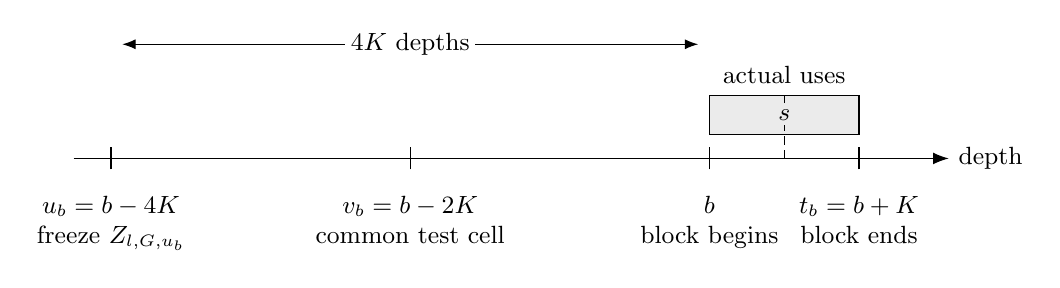
\begin{tikzpicture}[x=0.95cm,y=1cm,every node/.style={font=\small}]
  \draw[-{Latex[length=2mm]}] (0,0.8)--(11.7,0.8) node[right]{depth};
  \foreach \x in {0.5,4.5,8.5,10.5} {\draw (\x,0.66)--(\x,0.94);}
  \draw[fill=black!8] (8.5,1.1) rectangle (10.5,1.6);
  \draw[densely dashed] (9.5,0.8)--(9.5,1.6);
  \node[fill=black!8,inner sep=1.5pt] at (9.5,1.35) {$s$};
  \node at (9.5,1.86) {actual uses};
  \draw[{Latex[length=1.7mm]}-{Latex[length=1.7mm]}] (0.65,2.25)--(8.35,2.25);
  \node[fill=white,inner sep=2pt] at (4.5,2.25) {$4K$ depths};

  \node[anchor=north,align=center] at (0.5,0.45)
       {$u_b=b-4K$\\freeze $Z_{l,G,u_b}$};
  \node[anchor=north,align=center] at (4.5,0.45)
       {$v_b=b-2K$\\common test cell};
  \node[anchor=north,align=center] at (8.5,0.45)
       {$b$\\block begins};
  \node[anchor=north,align=center] at (10.5,0.45)
       {$t_b=b+K$\\block ends};
\end{tikzpicture}

\caption{The depth convention of the first-match construction in
\cite[Section~8]{H}.  In the analysis block \([b,b+K)\), the basic
output in slot \(l\) is frozen at \(u_b=b-4K\), tested on common
cells at \(v_b=b-2K\), and used at actual depths
\(b\le s<t_b=b+K\).  The deterministic input block partitions in
Theorem~\ref{thm:depth-local} need not align with these analysis blocks.}
\label{fig:frozen-depths}
\end{figure}

A primary in this mode construction is an individual main column
\(\Phi\) matched to the maximal pad of the role's outer ball
filter.  At its first match on a cell \(I_0\), the
\emph{First-match expansion and bounded lift} Lemma of
\cite[Section~8]{H} chooses a finite list of augmented modes.
For each prospective branch offset \(\rho\), the modes use H's
cutoff \(\zeta^\rho\) and gauge \(p^\rho\) in the form
\[
 \psi_m(y)=
 \left(\zeta^\rho(y)e(\kappa_l p^\rho(y))
       e(\lambda_m y^2+\gamma_m y),
       \sqrt{\epsilon_{\rm m}}\,\mathbf e_m\right).
\]
The list, its labels, and its scalar expansion coefficients
\(a_{\Phi,m}\) are retained on every relevant descendant of the
first match; separate first-match branches may use separate private
labels.  They are not resampled at later freezing times, including
when a coefficient subsequently frozen is zero.  All modes of
one primary have one \(\lambda_m\).  The quantities
\(|\lambda_m||I_0|^2\), \(\sum_m|a_{\Phi,m}|\), their number, and
the heights of their relative linear-frequency vectors are bounded
by a quantity whose logarithm is polynomial in \(P,k\).

For a fixed prospective offset the same source Lemma gives one
pointwise bounded linear map \(\mathcal R_{l,G}\), fixed across
blocks.  On an outer main output
\(\sum_\Phi\beta_\Phi\Phi\) with coefficients constant on an
endpoint cell, it gives exactly
\(\sum_{\Phi,m}\beta_\Phi a_{\Phi,m}\psi_m\).  Thus
\[
 \widetilde Z_{l,G,b}=\mathcal R_{l,G}Z_{l,G,u_b}
\]
has coefficients constant on its whole \(u_b\)-cell.  The mode
labels and their private coordinates use \(D_*\); the main
endpoint projections still use \(D_{\rm m}\).

Write \(\mathcal H_{\rm mode}\) for the augmented mode Hilbert space.

\begin{lemma}[Frozen composition with depth inputs]
\label{lem:h-frozen-composition}
Fix a slot, one search leaf and its color, and a prospective choice
of the offsets for its groups, with the corresponding block-independent
maps \(\mathcal R_{l,G}\).  For every group \(G\) of that color, let \(P_e\) be finitely many
local mode projections: \(P_e\) is the orthogonal projection in
\(L^2(J_e;\mathcal H_{\rm mode})\) onto constant-coefficient combinations
of the restrictions of its available augmented modes.  Extend it to
\(L^2(R;\mathcal H_{\rm mode})\) by restricting the input to \(J_e\)
and extending the output by zero.  Suppose these rows have joint squared
Bessel bound at most \(G_0\) in each group.

Suppose \(J_e\subseteq U_e\), where \(U_e\) is a main endpoint
cell with a downstream actual-use certificate and is usable for
each nonzero pad range contributing to
\(\overline L_{l,G,U_e}\).  The row's mode labels are available
already at \(U_e\).  Write
\[
 B_{l,U_e}=\sum_{\tau=1}^{h_0}\varepsilon_\tau
       Q^\tau_{l,U_e}F_{l,s(U_e)},\qquad h_0\le2,
\]
for its specified basic-\(B\) expression, and let
\(\mathcal B_{l,U_e}\) be the shared main history of the leaf.
Then
\begin{equation}
 \sum_{G,e}
 \|P_e\mathcal R_{l,G}\overline L_{l,G,U_e}
                  \mathcal B_{l,U_e}B_{l,U_e}\|_2^2
       \le G_0|R|.
 \label{eq:h-frozen-composition}
\end{equation}
Endpoint depths may be arbitrary and need not be current; any
number of rows may share one endpoint cell.  The bound is uniform
in the prospective choices of offsets.
\end{lemma}

\begin{proof}
We first form an ordinary joint Bessel operator using the fixed
lift, outer main projections, and usable-endpoint synthesis.
We then insert the shared histories and the constituent basic
projection, and only afterward evaluate the rows on their varying
endpoint inputs.

For a fixed group the rows \(P_e\mathcal R_{l,G}\) are Bessel
because \(\mathcal R_{l,G}\) is one fixed bounded operator.  They
are local to \(J_e\), hence to the containing decision cell
\(U_e\).  Compression inserts an outer individual main projection
on \(U_e\); the triangle inequality in the finite Hilbert sum of
rows restores its positive average.  If \(A_G\) denotes this row
operator, an individual row adjoint has the order
\[
 L_{l,G,U_e}\mathcal R_{l,G}^*P_e.
\]
Its range is the main ball range on the whole \(U_e\).  The pad
usability hypothesis and \eqref{eq:h-usable-synthesis} therefore
give
\[
 \left\|\sum_G A_G^*w_G\right\|_2^2
 \le C\sum_G\|A_G^*w_G\|_2^2
 \le G_0\sum_G\|w_G\|^2.
\]
By duality, the ordinary rows are jointly Bessel across all groups
and rows.  Their use of the whole endpoint \(U_e\) is the reason
the synthesis bound applies despite the smaller output cell \(J_e\).

Apply Compression again at the decision cells \(U_e\) to insert
the shared histories and one fixed basic constituent.  Expand
complements into their signed ordered products and retain
normalized positive averages.  For each coupled expanded term,
the resulting ordinary rows \(T_e\) satisfy
\begin{equation}
 \sum_{G,e}\|T_e h\|_2^2\le G_0\|h\|_2^2
 \quad\text{for every }h\in L^2(R;\mathcal H).
 \label{eq:h-frozen-operator}
\end{equation}
Every nonzero basic constituent has its input-side projection
\(Q^\tau_{l,U_e}\), even if all other selected factors are
identities.  Thus the final action of \(T_e^*\) is
\(Q^\tau_{l,U_e}\), and its range is a main-catalog combination
on the entire \(U_e\).  The composed row has input support on
\(U_e\).  Grouping rows by \(s(U_e)\), the full depth partition
serves as both input-support and observation partition, and the
read is \(F_{l,s(U_e)}\).  These partitions refine and the read
indices increase.  Equation~\eqref{eq:h-row-use}, applied to
\eqref{eq:h-frozen-operator} with budget \(D_{\rm m}\), proves
\eqref{eq:h-frozen-composition} after restoring the controlled
signed terms and averages.

The mode projections entered the ordinary Bessel operator before
this last evaluation.  The final adjoint range is the basic main
range on \(U_e\), so the row estimate uses \(D_{\rm m}\).  For a
row from block \(b\), its read and observation depth are
\(s(U_e)=u_b\), regardless of the later mode-output cell \(J_e\)
or the actual use depth.
\end{proof}

Lemmas~\ref{lem:h-certified-variation} and
\ref{lem:h-frozen-composition} now provide the cross-depth
variation and frozen-evaluation bounds needed for H's mode split.
We next verify the resulting side energy and component data.

\subsection{Side and core data from the frozen modes}

Fix a prospective choice of the group offsets.  On each retained \(v_b\)-cell, make
H's permitted choice to keep the full available mode list frozen
at \(u_b\), including every matched primary and every
zero-coefficient label.  PRE and CURRENT mean exactly the graphs
of Equation~\Heq{22} in \cite[Section~8]{H} on that list and that
same \(v_b\)-cell.  Their edge tests use the supremum of the
affine-slope difference
\(\omega_m(x)-\omega_{m'}(x)\), where
\(\omega_m(x)=2\lambda_mx+\gamma_m\), after the source's permitted
integral shifts.  The comparison scales are \(r_{v_b}\) for PRE
and \(r_{t_b}\) for CURRENT.  A minimal PRE component and a minimal
CURRENT component are their respective height-zero components.
Available lists and old labels persist on relevant descendants;
admitted edges persist or grow as the source height or descendant
block advances.

We retain H's source-defined good predicates and core/side
classification.  The \emph{Coherence of good predicates} Lemma
says that a minimal PRE component classified as side consists
entirely of side modes.  It also says that the upper good-height
masks select unions of complete core subtotals inside minimal
CURRENT components.  A minimal CURRENT component may contain
side modes as well.  At an upper height, a successful CURRENT
component means one containing a core mode good at that height;
its good modes have one PRE predecessor at the prescribed lower
height.

For a \(B\) role, let \(V_{l,G,b}\) be the exact subtotal of the
side modes of \(\widetilde Z_{l,G,b}\), including their private
coordinates, on retained \(v_b\)-cells.  Set it to zero on branches
without a needed output or certificate.  For the fixed prospective
offset it is one fixed function throughout the block.  We verify
the source square-energy estimate for these new frozen operands.

An event in the proof of \emph{Square energy of the linear side}
in \cite[Section~8]{H} consists of a block, a retained \(v_b\)-cell
\(J\), and a minimal PRE component \(\mathcal E\) of side modes.
The \emph{Separated mode rows} Lemma and the
\emph{Bad-density chains} Lemma organize its projection rows into
ten block congruence classes and
\(O(d_{\max}\log(2D_{\rm m}))\) chain levels.  The source chain
calculation absorbs its larger mode-height parameter before this
final length bound.  Thus the per-group squared Bessel cost is
\(G_0\).  Lemma~\ref{lem:h-frozen-composition}, with \(U_e\) the
containing \(u_b\)-cell, gives the source Equation~\Heq{24}:
\[
 \sum_{G,b,J,\mathcal E}
       \|P_{\mathcal E,J}\widetilde Z_{l,G,b}\|_2^2
       \le G_0|R|.
\]
Here \(P_{\mathcal E,J}\) is the local projection onto that
component's augmented modes.  If \(T_{\mathcal E,J}\) is its
exact coefficient subtotal, the source separation and the bound
\(\sum_m|\alpha_m|\le D_*\) on the frozen cell give
\[
 \|P_{\mathcal E,J}\widetilde Z-T_{\mathcal E,J}\|_{2,J}
       \le D_*^{-190}.
\]
The path budgets sum these additive errors.  Almost orthogonality
of the distinct minimal PRE subtotals then yields
\begin{equation}
 \sum_{G,b}\|V_{l,G,b}\|_2^2\le G_0|R|.
 \label{eq:h-linear-energy}
\end{equation}
This deduction is uniform in the prospective choices of offsets.  It uses the
persistent lists and graphs and each endpoint's own coefficient
subtotal; it requires no relation between coefficients frozen in
different blocks.

Let \(A_{l,G,b}\) be the exact core subtotal.  In a \(B\) role
define
\[
 S^{\rm roll}_{l,G,s}=Z_{l,G,s}-Z_{l,G,u_b},\qquad
 S_{l,G,s}=S^{\rm roll}_{l,G,s}+V_{l,G,b},
 \quad b\le s<b+K.
\]
The physical identity in
\emph{Fixing offsets and separating the side terms} of
\cite[Section~8]{H} is
\begin{equation}
 \begin{gathered}
 (Z_{l,G,s})_{\rm phys}
   =(A_{l,G,b})_{\rm phys}+(S_{l,G,s})_{\rm phys}
          +\mathcal E_{l,G,b},\\
 \mathcal E_{l,G,b}
   =(Z_{l,G,u_b})_{\rm phys}
          -(\widetilde Z_{l,G,b})_{\rm phys}.
 \end{gathered}
 \label{eq:h-core-side}
\end{equation}
In a basic-\(U\) role there is no core: set
\(S_{l,G,s}=Z_{l,G,s}^{\,U}\) and take no physical error.
The core and side subtotals retain their augmented coordinates
in all norm estimates.

This decomposition determines the remaining estimates.  Terms
with at least three side positions will use their path-square
bounds at a power \(p\in(2/3,1)\).  Terms with exactly two sides
will restore the two whole current complements and use filter
transfer.  Terms with at least three cores will use H's
conditional counting estimate.  For a powered within-cell group
contribution \(x\), the truncation gives
\(\min(\eta,x)\le\eta^{1-p}x^p\).  The transfer's bands with
adjacent pad indices will be estimated at power one, with their
prescribed fixed-offset sums kept inside the cell.

It remains to select the offsets.  The main catalogs, the
coefficients \(\beta_\Phi\) in
\(Z_{l,G,u_b}=\sum_\Phi\beta_\Phi\Phi\) on each whole \(u_b\)-cell,
and all actual main uses were fixed before the prospective
offsets.  With the source accuracy \(\delta_c=\exp(-k^{C_c})\),
where \(C_c\) is chosen after the main budgets, H's explicit lift
and offset average give
\[
 \mathbb E_\rho\sum_{l,G,I\ {\rm used}}|I|
       \|\mathcal E_{l,G,b(I)}\|_{2,I}^2
 \le D_{\rm m}^C d_{\max}\delta_c\,|R|.
\]
This sum is over all those pre-existing actual uses, before any
offset-dependent cuts.  The coefficient and physical supremum
bounds are on the whole \(u_b\)-cell.  By
\eqref{eq:h-input-size}, its operand \(F_{l,u_b}\) has normalized
norm at most one, so the lag \(4K\) introduces no size factor.
Choose offsets satisfying the displayed bound, with the
inverse-main-budget accuracy \(\delta_c\) prescribed by H.
The uniform estimate \eqref{eq:h-linear-energy} remains valid
for this choice, and subsequent pruning only removes terms from
the nonnegative error sum.

The chosen whole augmented states \(S_{l,G,s}\) are now fixed.
Realize H's helper closure on these states and their named
histories by the same fixed-base calculation
\eqref{eq:h-closure-test}--\eqref{eq:h-closure-prefix}.  There
are at most \(\exp(C_qk^C)\) such bases per active cell over the
specified slots, groups, and patterns.  They are whole states,
with no choice of a mode, height, or amplitude as a helper base.
Their existing private coordinates are distinct from the fresh
helper directions.  This realizes the anticipated helper count
within \(D_{\rm m}\).  The dependent size and counting cuts
described next are imposed after these choices.

The separate integrated square bounds for the side components
follow from the two new lemmas and the basic energy.  For the
rolling component, apply \eqref{eq:h-certified-variation} to
\([u_b,s]\), \(b\le s<b+K\), with the unions of actual \(s\)-cells
as endpoint sets; these intervals have \(O(K)\) overlap.  At each
depth the use cells for fixed \(G,b\) are disjoint, so a fixed
\(V_{l,G,b}\) is counted at most \(K\) times.  In a \(U\) role,
\eqref{eq:h-usable-rows} at each depth and the basic energy in
\eqref{eq:h-base-data} bound the current outputs.  Consequently
\begin{equation}
 \begin{aligned}
 \sum_{s,G}\sum_{I\ {\rm used\ at}\ s}|I|
       \|S^{\rm roll}_{l,G,s}\|_{2,I}^2
       &\le CK G_0|R| &&\text{in a \(B\) role},\\
 \sum_{s,G}\sum_{I\ {\rm used\ at}\ s}|I|
       \|V_{l,G,b(s)}\|_{2,I}^2
       &\le K G_0|R| &&\text{in a \(B\) role},\\
 \sum_{s,G}\sum_{I\ {\rm used\ at}\ s}|I|
       \|S_{l,G,s}\|_{2,I}^2
       &\le P^C|R| &&\text{in either role},\\
 \sum_{s,G}\sum_{I\ {\rm used\ at}\ s}|I|
       \|Z^{\,U}_{l,G,s}\|_{2,I}^2
       &\le G_0|R| &&\text{in a \(U\) role}.
 \end{aligned}
 \label{eq:h-side-square}
\end{equation}
The first two inequalities concern a \(B\) role.  Their sum
bounds its whole \(S\) by the squared triangle inequality.
The fixed polynomial in \(k\) from the basic energy is included
in \(G_0\).

H's componentwise first-crossing construction in
\cite[Section~7, Side estimate]{H} applies to this finite list of
components.  Apply it separately to the nonnegative partial path
sums for \(S^{\rm roll}\), for the repeated \(V\), and for the
basic-\(U\) output when present, using their respective integrated
bounds above.  By increasing the thresholds by fixed factors,
their first-crossing cells have any prescribed small fixed total
relative length.  On the retained paths this gives
\begin{equation}
 \begin{aligned}
 \sum_{s,G}\|S^{\rm roll}_{l,G,s}\|_{2,I_s(x)}^2
       &\le P^C &&\text{in a \(B\) role},\\
 \sum_{s,G}\|V_{l,G,b(s)}\|_{2,I_s(x)}^2
       &\le P^C &&\text{in a \(B\) role},\\
 \sum_{s,G}\|Z^{\,U}_{l,G,s}\|_{2,I_s(x)}^2
       &\le P^C &&\text{in a \(U\) role},\\
 \sum_{s,G}\|S_{l,G,s}\|_{2,I_s(x)}^2
       &\le P^C &&\text{in either role}.
 \end{aligned}
 \label{eq:h-side-cap}
\end{equation}
Only actual uses are summed.  The final cap follows from the
separate component caps and
\(\|S^{\rm roll}+V\|^2\le2\|S^{\rm roll}\|^2+2\|V\|^2\).
The exponent may be increased for the polynomially many
configurations where a power cost is allowed.

These separate caps also give the local input for H's component
sizes.  At a retained \(B\) use, the current local size of \(Z_s\)
is bounded by contraction and \eqref{eq:h-base-data}.  The
bounded lift and \(Z_{u_b}=Z_s-S^{\rm roll}_s\) therefore give
\[
 \|\widetilde Z_{l,G,b}\|_{2,I}+\|V_{l,G,b}\|_{2,I}
 \le C\bigl(\|Z_{l,G,s}\|_{2,I}
             +\|S^{\rm roll}_{l,G,s}\|_{2,I}\bigr)
             +\|V_{l,G,b}\|_{2,I}
 \le P^C.
\]
The core subtotal \(A=\widetilde Z-V\) has the same type of local
bound.  H's local \(L^2\) form estimate and Cauchy--Schwarz over
the original actual uses now turn the selected integrated
physical-error bound into total absolute error \(O(e^{-k}|R|)\).

We next record the representative and top-count inputs for the
core calculation.  A successful component's type is the pair of
floor logarithms, to base \(1.1\), of its unique good PRE
predecessor's primary count and mode count.  For a fixed role,
group, upper height, and type, the
\emph{Hereditary representatives} Lemma of
\cite[Section~8]{H} chooses a mode label \(a\) in each such
predecessor and inherits it on later contained predecessors.
Write \(z\) for the group's primary center and \(\theta_z\) for
the horizontal vector in its tag.  H uses
\(\vartheta=\theta_z/Q_0\), where \(Q_0\) is H's denominator-clearing
integer common to the roles of this group.  Write \(L_h,E_h,\Xi\) for the
source shift denominator, shift range, and separation threshold.
For distinct representatives on comparable actual cells \(I,I'\)
and \(x_*\in I\cap I'\), it gives
\begin{equation}
 |\omega_a(x_*)-\omega_{a'}(x_*)+n\cdot\vartheta/L_h|
   >\frac{\Xi}{2}\max(|I|^{-1},|I'|^{-1})
 \quad(n\in\mathbb Z^{\dim\theta_z},\ |n|_\infty\le E_h).
 \label{eq:h-representative-separation}
\end{equation}
The identification across depths is the persistent mode label
and its value \(\omega_a(x_*)\).

For an actual cell \(I\) and a successful component
\(\mathcal F\), H uses
\[
 \sigma_{\mathcal F}^2
 =\sum_{\substack{\mathcal D\subseteq\mathcal F\\
                    \mathcal D\ {\rm minimal\ CURRENT}}}
    \left(\|A_{\mathcal D}\|_{2,I}
       +D_*^{-30}\!\!\sum_{\substack{m\ {\rm core}\\m\in\mathcal D}}
                         |\alpha_m|\right)^2.
\]
Here \(A_{\mathcal D}\) is the complete core subtotal within
\(\mathcal D\); side labels in that component are kept separately.
The \emph{Component-size comparison} Lemma of
\cite[Section~8]{H} gives the same-cell bounds
\[
 \sigma_{\mathcal F}^2
 \le C\bigl(\|P_{\mathcal F,I}\widetilde Z_{l,G,b}\|_{2,I}^2
             +\|V_{\mathcal F}\|_{2,I}^2+D_*^{-50}\bigr),
 \qquad
 \sum_{\mathcal F}\|V_{\mathcal F}\|_{2,I}^2
       \le C\|V_{l,G,b}\|_{2,I}^2.
\]
The projection \(P_{\mathcal F,I}\) uses all mode labels of
\(\mathcal F\) on \(I\), and \(V_{\mathcal F}\) is their exact
side subtotal.  This is an almost-orthogonality estimate for
arbitrary coefficient subtotals on one cell.

For a fixed source role, upper height, type, and dyadic threshold
\(D_*^{-1}\le\sigma\le D_*^2\), H takes, for each group and
representative, the first actual-use cells on each spatial branch
for which \(\sigma_{\mathcal F}\ge\sigma\).  Several incomparable
tops for the same group and representative are allowed.  The
resulting top rows
\(P_{\mathcal F,I}\) are separated mode rows.  They are supported
on \(I\subseteq U_e\), the \(u_b\)-cell of the frozen list, and
the top itself is a downstream certificate.  Applying
Lemma~\ref{lem:h-frozen-composition} gives squared energy
\(G_0|R|\) for their frozen projections.  Summing the side
term of the size comparison first at one depth and then through
a block gives at most
\(K\sum_{G,b}\|V_{l,G,b}\|_2^2\le KG_0|R|\).  The
\(D_*^{-50}\) floor is absorbed because
\(\sigma^2\ge D_*^{-2}\).  Hence
\[
 \sigma^2\sum_{\rm tops}|I|\le C(1+K)G_0|R|.
\]
There are polynomially many choices in \(P,k\) of height, type,
and threshold.  The first-crossing construction of the
\emph{Top count} Proposition in \cite[Section~8]{H} gives, on
retained paths,
\begin{equation}
 \sum_G|\mathcal A_j^G|
       \le\min(D_*,P^C\sigma_j^{-2}).
 \label{eq:h-top-count}
\end{equation}
Here \(\mathcal A_j^G\) is the set of distinct representatives
actually used in the bin \([\sigma_j,2\sigma_j)\) along the retained
path in question, for the fixed role, height, and type.  The full
label budget supplies the
minimum for \(\sigma_j<D_*^{-1}\); bins above the tested range
are empty after the source budget enlargement.  Finally, the
local bounds on \(\widetilde Z\) and \(V\) above and the
component-size comparison give \(\sigma_{\mathcal F}\le P^C\)
on retained uses.  These are the local sizes and role counts
needed by the core calculation.

\subsection{The side estimate}

We use the \emph{Side estimate} Proposition of \cite[Section~7]{H}, with the
component bounds just verified.  Suppose first that three
positions have sizes whose path squares obey
\eqref{eq:h-side-cap}.  Along a path put \(a_s=(\sum_Ga_{s,G}^2)^{1/2}\)
and define \(b_s,c_s\) analogously, using a shared size directly
when appropriate.  Cauchy--Schwarz in the group index
bounds the absolute group sum by \(P^C a_sb_sc_s\), using the
retained bound \(P^C\) for the fourth local size.  For
\(2/3<p<1\), Hölder and \(3p>2\) give
\[
 \sum_s(a_sb_sc_s)^p
 \le
 \left(\sum_sa_s^2\right)^{p/2}
 \left(\sum_sb_s^2\right)^{p/2}
 \left(\sum_sc_s^2\right)^{p/2}.
\]
Integrating the path caps therefore gives total length-weighted
\(p\)th-power cost \(P^C|R|\).  The power is taken after the
group sum at each original cell.

For exactly two sides, replace their two core complements in
\eqref{eq:h-core-side} by the whole current \(Z\) arguments.
The corrections have a third side, apart from the physical errors
already estimated.  We recall the source filter algebra for these
whole complements.  Let the side positions be \(a,b\) and the
complementary positions be \(c,d\).  Expand each complementary
factor \(1-\overline Q\) as identity minus a positive average.
The \emph{Outgoing filters and near-band defects} Lemma of
\cite[Section~6]{H} removes the positive filters from \(c,d\)
in decreasing rank and transfers helper averages to the fixed
whole state \(S_a\).  Its final main term is
\[
 H_I(\mathcal D_{a,s}S_a,S_b,B_c,B_d),
\]
where \(\mathcal D_{a,s}\) has \(O(\log\mathcal L)\) helper
factors.

For one step from \(c\) to \(a\), write \(Q_{l,p}\),
\(1\le p\le P\), for the outgoing and corresponding helper
projections, and put
\[
 Q_{l,0}=0,\quad Q_{l,P+1}=1,\quad
 A_l^p=Q_{l,p}-Q_{l,p-1},\quad
 \overline Q_l=P^{-1}\sum_{p=1}^P Q_{l,p}.
\]
Here \(x_c\) is the exact remaining input-side source history
on \(B_c\), \(x_d\) is the whole remaining history on \(B_d\),
\(x_a\) is the already transferred helper history on \(S_a\),
and \(x_b=S_b\).  The exact difference is
\begin{equation}
 H_I(x_a,x_b,\overline Q_cx_c,x_d)
       -H_I(\overline Q_ax_a,x_b,x_c,x_d)
 =\sum_{p,q'=1}^{P+1}\frac{p-q'}P
       H_I(A_a^p x_a,x_b,A_c^{q'}x_c,x_d).
 \label{eq:h-transfer}
\end{equation}
The pad projections are nested on this cell, so the \(A_l^p\)
are orthogonal bands summing to the identity.  The average has
weight \((P-p+1)/P\) on band \(p\), which proves the identity.
H's closure and tag-separation estimates bound the sum with
\(|p-q'|>2\) by
\(D_{\rm base}^{-C_3}\|S_a\|_{2,I}\|S_b\|_{2,I}\), for any
prescribed fixed \(C_3\) after choosing its numerical accuracies.
The helper closure here uses the already fixed whole \(S_a\)
as its base in \eqref{eq:h-closure-test}.  For the retained terms,
keep the entire band sum at each fixed offset \(q'-p\).

In the final main term, write \(B_c=Y_c-U_c\) and
\(B_d=Y_d-U_d\).  Each correction has a third basic side.
The remaining complementary pair \(Y_c,Y_d\) has form norm at
most \(\eta\) against the two side inputs, by the full-pair
statement of Proposition~\ref{prop:hbase-data}.  Contraction of
the helper factors and Cauchy--Schwarz in the side sizes give
absolute main cost \(\eta P^C|R|\).  The numerical transfer
errors are summable with the chosen inverse-base-budget accuracy.

For a retained offset, write
\(C_{G,s}^{q'}=A_c^{q'}x_{c,s}\) for the outgoing complementary
band stack and \(D_{G,s}=x_{d,s}\) for the other complement.
Freeze both at the block start \(b\), using their full endpoint
evaluations there.  These endpoints differ from the mode
freezing depth \(u_b\).  Corollary~\ref{cor:h-transfer-endpoint-variation}
applies to exactly these source histories.  For a ball transfer,
a nonterminal band is the difference of two eligible positive
ball endpoints; its terminal band is the shared inner history
minus the positive \(P\)-pad endpoint.  For a cumulative transfer,
the outer ball has already been removed and all the complementary
endpoints are shared.  The other complement has its one source
positive outer ball or is shared.  Thus each band costs a fixed
multiple of its endpoint estimates, and the shared histories
are counted once across their uses.  Summing the \(P+1\) bands
and the \(O(K)\) overlap of \([b,s]\) retains the allowed
polynomial cost \(P^C|R|\).
Their nonnegative partial path sums enter the power-cost first-crossing
cuts.

At a required endpoint the pad bands are orthogonal, and the
remaining source histories are contractions of bounded basic
inputs.  Choose \(C_{\rm fr}\ge1\) to dominate the retained
current local norm of the band stack and of the other complement.
A freeze error has a third path-square size by the preceding
endpoint bounds.  If the other frozen complement is large,
write it as its bounded current value plus its difference.
Likewise, if a frozen local size exceeds \(2C_{\rm fr}\) while
the current one is at most \(C_{\rm fr}\), then the difference
exceeds \(C_{\rm fr}\), and the flag is at most
\(C_{\rm fr}^{-2}\) times the squared difference size.  Its square root is therefore
another path-square size.  Certified variation applies on the whole ancestor cells with downstream
certificates; propagation through a block costs at most \(K\)
in this power budget.  H's freeze, large-complement, and
restoration errors therefore have total \(p\)th-power cost
\(P^C|R|\).  A large-complement flag is charged to that error
sum; only a first crossing of its accumulated budget makes a
restart cut.  On the remaining uses the frozen complements have
bounded local sizes on their entire ancestor hulls in the block.

\subsubsection{Fixed stacks for the two side inputs}

Fix a source transfer step, a near offset, and a search leaf.
Under these fixed data, let \(\chi\) record the source auxiliary
side-component and binary-length names for the two side stacks.
Pairing their choices raises the auxiliary count to a fixed power,
so a common auxiliary list has at most \(G_0\) entries after enlarging \(G_0\) within
its stated class; unused combinations are set to zero.  Write
\(\nu=(G,b,\chi)\) for the full stack index.  Concrete binary
interval positions and band labels \(p\) are stack coordinates,
and individual pads remain in coupled averages.  For one full
index, a stored side stack is a function into a finite Hilbert
direct sum:
\[
 \begin{gathered}
 \mathrm{stack}_{\mathrm{untouched},\nu}(y)
       =(W_{\nu,i}(y))_{i\in\mathcal I_\nu}
       \in\bigoplus_{i\in\mathcal I_\nu}\mathcal H,\\
 \|\mathrm{stack}_{\mathrm{untouched},\nu}\|_2^2
       =\sum_i\|W_{\nu,i}\|_2^2.
 \end{gathered}
\]
The banded stack \(\mathrm{stack}_{a,\nu}\) has in addition the
band index \(p\in\{1,\ldots,P+1\}\).  Here \(\mathcal H\) is the
augmented ambient Hilbert space of the stored coordinates.  Each
whole coordinate is restricted, when formed, to the union of the
use cells selecting its position and valid band.  Later cuts
remove summands without changing that stored function.  At a use,
each side selects one position; the banded side retains all valid
matched band indices at the fixed offset.

The source stack construction gives the squared energies
\begin{equation}
 \sum_\nu\|\mathrm{stack}_{a,\nu}\|_2^2\le PG_0|R|,
 \qquad
 \sum_\nu\|\mathrm{stack}_{\mathrm{untouched},\nu}\|_2^2\le G_0|R|.
 \label{eq:h-stacks}
\end{equation}
Both sums range over all full indices \(\nu=(G,b,\chi)\).
The \(G_0\) cardinality overhead counts only the auxiliary labels
\(\chi\); both energies sum all groups and blocks.
Their quantitative purpose is the following.  The whole-hull
maximal and sparse calculation below turns these energies into
a root-size sum with cost \(P^{1/2}G_0|R|\).  The coefficient
\(O(P^{-1})\) in the matched transfer bands then leaves the
gain \(P^{-1/2}\).  We first check the fixed-vector arguments
behind \eqref{eq:h-stacks}.

For a sequence \(W_s\) in one block, write
\[
 W_s=W_b+\sum_{[r,t]\in\mathcal P(b,s)}(W_t-W_r),
\]
where \(\mathcal P(b,s)\) is the binary decomposition of the
prefix.  At a fixed length its intervals are disjoint and at
most one is selected at a use.  Store each resulting function
on its selecting-use union as above.  For a basic-\(U\) side,
store each already formed depth function directly;
\eqref{eq:h-side-square} bounds its energy, and subsequent
helper products are local contractions.

For a linear side \(V_{G,b}\), let \(T_s\) be the product of
the subsequent helper projections, including one endpoint of
a band difference when needed.  The products-of-prefixes
estimate of \cite[Section~3]{H}, on at most \(K+1\) times, gives
for each fixed binary length
\[
 \|T_bV_{G,b}\|_2^2+
 \sum_{[r,t]\ {\rm at\ that\ length}}
       \|(T_t-T_r)V_{G,b}\|_2^2
 \le (C\log(K+2))^{O(m)}\|V_{G,b}\|_2^2.
\]
The input \(V_{G,b}\) is the one fixed function on the block.
Use \eqref{eq:h-linear-energy}, sum the logarithmic length
choices, and pay at most \(P+1\) band indices for the first
stack.

For a rolling side put \(W_s=T_s(Z_{G,s}-Z_{G,u_b})\).
Its base value uses \eqref{eq:h-certified-variation} on
\([u_b,b]\), whose overlap across blocks is bounded.  Its
increments split exactly as
\[
 W_t-W_r=T_t(Z_{G,t}-Z_{G,r})
             +(T_t-T_r)(Z_{G,r}-Z_{G,u_b}).
\]
The first term uses certified variation on the whole endpoint
cells containing its selected use cells.  For the second, also
decompose \([u_b,r]\) into binary intervals.  Fix an outer
length, an inner length, and an inner interval \([a,v]\).
Every outer position selecting this interval acts on the one
fixed function
\[
 X=\mathbf1_\Omega(Z_{G,v}-Z_{G,a}),
\]
where \(\Omega\) is the union of its required \(r\)-cells.
Since \(v\le r\), locality of \(T_t-T_r\) gives the required
outputs from \(X\).  Enlarge \(\Omega\) to the containing whole
\(v\)-cells to bound its norm; those cells have downstream
certificates.  The fixed-vector product-jump estimate sums the
outer positions by
\((C\log(K+2))^{O(m)}\|X\|_2^2\).  Then
\eqref{eq:h-certified-variation} sums these squared inputs over
groups and the disjoint inner intervals at that length.  The
\(O(K)\)-depth windows for different blocks have bounded
overlap.  The two endpoint outputs in \(X\) use \(F_v\) and
\(F_a\), but \(X\) itself is fixed once \(a,v\) are fixed, as
required for the outer product-jump estimate.

This proves \eqref{eq:h-stacks}.  Coupled pad averages are restored
by Jensen's inequality.  When the fixed search-leaf and transfer-step
choices are restored later, their auxiliary overhead fits an enlarged
\(G_0\).

We collect the main-row and stack costs here.  For
\(m=O(\log\mathcal L)=O(\log k)\), the Compression factor in
\eqref{eq:h-compression} satisfies
\[
 \log\mathfrak C(m,D_{\rm m})
 \le C(m+1)\bigl(\log(m+1)+\log\log(2D_{\rm m})\bigr)
 \le C_q(1+\log(2k))^C.
\]
A row application loses \(\log(2D_{\rm m})\) in norm, hence
\(\log^2(2D_{\rm m})\) in squared energy.  This loss, the
controlled signed expansions, and the telescoping counts fit
\(G_0\).  The factors \((C\log(K+2))^{O(m)}\) and the binary
length choices also fit \(G_0\) by
\eqref{eq:h-budget-hierarchy}.  Thus no fixed power of \(K\)
enters \eqref{eq:h-stacks}.  Its powers in the component and
top bounds stay in the allowed \(P^C\) budgets.  The larger
\(D_*\) is used in the mode construction, Bessel, and counting arguments;
the final row adjoints in the two new lemmas use \(D_{\rm m}\).

\subsubsection{The fixed-input comparison on a short block}

For \(2<q<3\), put \(M_qg=(M(|g|^q))^{1/q}\), where \(M\) is
the uncentered Hardy--Littlewood maximal operator.  For every
integer \(N\ge1\), let \(C_N(q)\) be the least constant such that
\begin{equation}
 \sum_{I\in\mathcal A}|I||H_I(g_0,g_1,g_2,g_3)|
 \le C_N(q)\int_{\mathbb R}\prod_{j=0}^3M_qg_j
 \label{eq:h-fixed-local}
\end{equation}
for every dyadic lattice, finite collection \(\mathcal A\) in
at most \(N\) consecutive depths, admissible kernel family, and
four compactly supported scalar \(L^q\) functions \(g_j\) fixed
across the collection.  The \emph{Local absolute estimate} Lemma of H gives
\(C_N(q)\le CN\), so this constant is finite before its uniform
bound is used.

For our application choose \(N=d+1\), where \(d\) is the largest
original depth in Theorem~\ref{thm:depth-local}.  The summation
cells in each short-block piece are retained original active cells,
with their original depths in \(\{0,\ldots,d\}\).  Restarts only
change their assigned attempt.  Hull ancestors and completion
leaves, including a boundary level one step below a block, supply
the geometry and leaf norm conditions; they are not additional
form summation cells.

We use the following specialization of the
\emph{Short-block comparison} Lemma of \cite[Section~7]{H}.
Let a finite tree piece have internal summation cells in at most
\(K\) consecutive depths of this original \(N\)-depth range and
leaves in that block or one depth below.  Let deterministic
Hilbert-valued stacks \(\mathbf z_j\), supported on its root \(Q\),
satisfy \(\|\mathbf z_j\|_{2,L}\le s_j\) on every leaf \(L\).
Suppose scalar randomizations \(z_j^\sigma\) satisfy, for every
finite real \(a\ge1\),
\[
 \bigl(\mathbb E_\sigma|z_j^\sigma(y)|^a\bigr)^{1/a}
       \le C_a\|\mathbf z_j(y)\|
 \quad\text{for almost every }y,
\]
with \(C_a\) independent of the tree and \(K\).  Then, for
arbitrary measurable signs \(|\epsilon_I(\sigma)|\le1\) and any
subcollection of the internal cells,
\begin{equation}
 \mathbb E_\sigma\left|
   \sum_I|I|\epsilon_I(\sigma)
          H_I(z_0^\sigma,\ldots,z_3^\sigma)\right|
 \le (1+C_N(q))C_q(1+\log(K+2))^C
       (K+2)^{C_{19}(q-2)}|Q|\prod_j s_j.
 \label{eq:h-short-block}
\end{equation}
The degree \(C_{19}\) is absolute.  Products of at most two
independent Rademacher randomizations of a finite vector stack
satisfy the stated moment hypothesis.

Apply this comparison to the stacks in \eqref{eq:h-stacks},
the frozen complementary band stack, and the other frozen
complement.  The scalar inputs are sums of their physical
components.  Use independent signs \(\varepsilon_i,\eta_j\)
for the two position indices and signs \(\zeta_p\) for the
band index.  At the fixed offset \(\ell=q'-p\), index the complementary
coordinate \(q'=p+\ell\) by \(p\).  Randomize the banded side
by \(\varepsilon_i\zeta_p\), the untouched side by \(\eta_j\),
and that complementary band coordinate by \(\zeta_p\).  At a
use put \(\varepsilon_{i(s)}\eta_{j(s)}\) in the kernel.
Expectation selects the two positions and all matched bands,
leaving \((p-q')/P=O(P^{-1})\).  Iterated Khintchine
inequalities bound every finite scalar moment by the augmented
stack norm.

After fixing the signs, these randomized physical stack sums are
fixed scalar \(L^2\) functions.  As a randomized family, they satisfy
the pointwise moment bounds for every finite \(a\ge1\), controlled by
the deterministic stacks with the stated leaf sizes; the randomizations are not asserted to
lie in \(L^q\).  In H's \emph{Return to the continuous form by
bursts} step, fix the auxiliary random and fast parameters outside
a null set.  The burst inputs are then finite scalar linear
combinations of indicators of bounded intervals with finite
coefficients.  They are therefore compactly supported \(L^q\)
functions fixed across the original summation cells.  H applies
\eqref{eq:h-fixed-local} to these inputs with the original admissible
kernels and then integrates the auxiliary parameters.  The clipping
and mixed-maximal calculation in that proof gives the exact block
power \((K+2)^{11(q-2)/(q-1)}\le(K+2)^{11(q-2)}\); the remaining
block factors are logarithmic.

For the whole-hull calculation, let \(\Omega_\nu\) be the union
of the use cells for one full index \(\nu=(G,b,\chi)\).  Its
maximal use cells are disjoint roots, and the hull contains every cell
between those roots and their uses.  For the already fixed stack
define
\[
 m_\nu^{\rm full}(x)=
 \sup_{\substack{I\ {\rm in\ the\ full\ hull}\\x\in I}}
       \fint_I\|\mathrm{stack}_\nu\|^2.
\]
Set \(m_\nu^{\rm full}=0\) outside its hull.  The supremum is
defined on every whole hull cell, including branches below later cuts.
A zero-energy family contributes
nothing.  Otherwise suppose a family has total stack energy
\(E|R|\) with \(E>0\), and
\(\sum_\nu|\Omega_\nu|\le M_0|R|\), where
\(M_0\le\exp(C_qk^C)\) follows from the active cell/group path
counts and the auxiliary-choice overhead, with all groups and
blocks included in this support sum.  The dyadic maximal calculation
in
\cite[Section~7]{H} gives
\[
 \begin{aligned}
 \sum_\nu|\{m_\nu^{\rm full}>T\}|
 &\le\min(M_0|R|,CE|R|/T),\\
 \sum_\nu\int_R\min(m_\nu^{\rm full},C_1E)
 &\le CE(1+\log(2+C_1M_0))|R|.
 \end{aligned}
\]
For a fixed sufficiently large \(C_1\), first-crossing cuts on the
individual and then joint partial ancestor suprema yield the retained caps
\[
 \sum_\nu m_{a,\nu}(x)\le PG_0,\qquad
 \sum_\nu m_{\mathrm{untouched},\nu}(x)\le G_0.
\]
Here \(m_{a,\nu},m_{\mathrm{untouched},\nu}\) use the retained hull cells, still
taken whole.  Include every potentially needed hull ancestor
within the block before these common cuts.  At a crossing the
cell is removed before its value enters a retained cap; below a
cut only earlier retained ancestors contribute.  The caps
therefore hold also on portions of retained hull cells below a
cut, with the small relative length cost supplied by the full
maximal bounds.

On each retained hull, make the source sparse decomposition:
from a root \(Q\), stop where either squared side average first
exceeds sixteen times its average on \(Q\).  A zero root average gives
zero contribution.  The stopped cells
have total length at most \(|Q|/8\), so the disjoint remainders
\(E_Q\) have measure at least \(7|Q|/8\).  Complete each piece
by children immediately below its included cells.  A child's
squared average is at most twice its parent's, which gives the
leaf bounds in \eqref{eq:h-short-block}; the frozen complementary
sizes are bounded on the whole hull and its boundary leaves.
If \(a_Q,b_Q\) are the side sizes at the piece roots, the
whole-hull convention puts \(Q\) in both suprema at every
\(x\in E_Q\), even below a cut.  Hence
\[
 \begin{split}
 \sum_{\nu,Q}|Q|a_Qb_Q
 &\le C\int_R\sum_\nu\sqrt{m_{a,\nu}m_{\mathrm{untouched},\nu}}\\
 &\le C\int_R
       \left(\sum_\nu m_{a,\nu}\right)^{1/2}
       \left(\sum_\nu m_{\mathrm{untouched},\nu}\right)^{1/2}
 \le P^{1/2}G_0|R|.
 \end{split}
\]
This is the promised root-size cost from the stack energies and
the whole-hull cuts.  Combining it with
\eqref{eq:h-short-block} and the matched coefficient \(O(P^{-1})\)
gives the near-band form of Equation~\Heq{19} of
\cite[Section~7]{H}:
\begin{equation}
 (1+C_N(q))C_qP^{-1/2}G_0
                  (K+2)^{C_{19}(q-2)}|R|.
 \label{eq:h-near-band}
\end{equation}
It bounds the absolute sum of original cell contributions with
the prescribed band sum retained inside each contribution at a
fixed offset.  The logarithmic block factors fit \(G_0\); the
displayed power of \(K+2\) comes from the fixed-input
short-block comparison.

\subsection{The core calculation}

The remaining terms have at least three core positions.  We
specialize the conditional calculation in
\emph{Counts for the tested core tuples} and
\emph{Powered estimate for the core terms} of
\cite[Section~9]{H}.  Its good-height predicates, shifted
annular tests, pure-shift gap, and numerical separation and
height reserves remain exactly those of the source construction.
We check the inputs that can be affected by the changed endpoint
operands.

Fix a retained path point \(x_*\), a group, an upper height,
role types, frequency bins \((\mu,\nu,\Lambda)\), and amplitude
bins \(\sigma_j\).  Let \(N_s^G\) be H's exact count of tested
core representative-label tuples at depth \(s\) for these data.
In a core role put \(M_j^G=|\mathcal A_j^G|\).  In the optional
side role put
\[
 M_l^G=\sigma_l^{-2}\sum_{s:\,G\ {\rm used}}
                 \|S_{l,G,s}\|_{2,I_s}^2,\qquad
 M'=\max_jM_j^G.
\]
Omit groups with no nonzero count, so \(M'\ge1\).  H's cell
calculation gives, apart from total absolute error
\(O(e^{-k}|R|)\), terms of the form
\[
 C_L\mu\nu^{-L}\Lambda^{-L}
            \left(\prod_{j=0}^3\sigma_j\right)N_s^G.
\]
Here \(0<\mu\le1\le\nu\) and \(\Lambda\ge1\) are dyadic, with
\(\Lambda=1\) for four core positions.  The good-height masks
select the full core subtotals within the minimal CURRENT
components, with the coefficient floor already included in
\(\sigma_{\mathcal F}\).

The preceding arguments provide the three inputs to the source count
that depend on endpoint data.  First, a
representative label has the fixed value \(\omega_a(x_*)\).
Distinct labels in one role obey
\eqref{eq:h-representative-separation}.  Together with H's exact
tested-tuple constraints, this ensures that two labels in distinct
core roles determine at most one tested tuple, and
the source height-bin estimate bounds its scale multiplicity.
Second, the frozen-row, component-size, and top argument gives
\eqref{eq:h-top-count}, including the \(D_*\) cap in each core
role.  Third, a side role uses the actual same-cell function
\(S_{l,G,s}\) in its Fourier windows.  Parseval gives its
incidence bound
\[
 w_s=\sigma_l^{-2}\|S_{l,G,s}\|_{2,I_s}^2,
\]
whose sum is \(M_l^G\) and whose path budget is supplied by
\eqref{eq:h-side-cap}.

The remaining hypotheses of the
\emph{Sparse mass of separated progression tests} Lemma of
\cite[Section~9]{H} are exactly H's shifted frequency tests
and pure-shift gap, retained from its construction.  As in its proof of
\emph{Counts for the tested core tuples}, every successful
component contains a nonexceptional primary, whose
pure-horizontal alternatives exclude the required intermediate
range for every permitted shift.  This is a property of the
persistent mode graph and its parameters.  The finite Lemma
therefore applies to the persistent labels and the actual
side incidences and gives, for an absolute \(p_0\in(0,1)\),
\begin{equation}
 \begin{gathered}
 \sum_sN_s^G\le L_0\min_{i\ne j}M_i^GM_j^G,\qquad
 L_0\le P^C(1+\log(\nu/\mu))^C,\\
 \sum_s(N_s^G)^{p_0}
 \le P^C(1+\nu+\mu^{-1}+\Lambda)^C(M')^{2p_0}.
 \end{gathered}
 \label{eq:h-core-counts}
\end{equation}
This source calculation identifies representative labels
across depths and uses same-cell side data; coefficients frozen
in different blocks may be unrelated.

Finally \eqref{eq:h-top-count} and \eqref{eq:h-side-cap} give
\(\sum_GM_j^G\le P^C\sigma_j^{-2}\) in every role, with the
additional \(D_*\) cap in a core role.  H interpolates the two
inequalities in \eqref{eq:h-core-counts}, keeps \(N_s^G\)
inside its power, and sums the amplitude and frequency bins.
Its \emph{Powered estimate for the core terms},
Equation~\Heq{37} of \cite[Section~9]{H}, gives absolute
constants \(\varepsilon>0\) and \(C_4\), with
\(p=1-\varepsilon>2/3\), and total contribution
\begin{equation}
 C_q\eta^\varepsilon P^{C_4}|R|+O(e^{-k}|R|)
 \label{eq:h-core-estimate}
\end{equation}
for the terms with at least three core positions on this
attempt's retained cells.  The original cell minimum is applied
before subadditivity and the group count remains inside the
power.  Numerical errors are estimated absolutely.  The
conditional source calculation thus uses the supplied persistent
labels, full core-subtotal masks, role counts, and actual side
Fourier data, with no further cross-depth estimate on an
original input.

\section{Completion of the local estimate}
\label{sec:completion}

\subsection{Restarts on the original summands}

We complete the target for a base segment \(R_0\) by the
construction in \cite[Section~10, One attempt and its restarts]{H}.
On an attempt \(R\), the main realization and actual uses precede
the prospective-offset calculation; the chosen whole sides then
precede helper closure and its dependent size and counting cuts.
The parent functions and operators remain fixed when original
summands are transferred at a cut.

The cuts accumulate nonnegative partial path counts, component
square sizes, or partial ancestor suprema.  Their integrated
bounds permit the thresholds to be increased by fixed factors.
Together with the initial marking-failure cuts, the union of first
stopped cells can then be chosen to have total length at most \(|R|/4\).
For the strong stack thresholds, only auxiliary choices contribute
a cardinality overhead, absorbed in \(G_0\); all full indices
\(\nu=(G,b,\chi)\) are controlled jointly by the aggregate energy
and full-hull bounds.  The polynomially many configurations in
\(P,k\) occur in the power budgets.  The hull construction
includes every potentially needed ancestor within a block before
the common cuts, and its maximal functions remain defined on
whole retained hull cells, including portions below a cut.
Large-frozen-complement flags are charged to the powered error
sum; only a first crossing of their accumulated budget creates
a restart root.

At a stopped cell \(R'\), send the original base summands there
and at its descendants to a fresh attempt.  Their original
depths, input schedules, and basic expressions remain assigned
to them.  The restrictions \(F_{j,s}|_{R'}\) satisfy the same
block normalization in each slot.  On \(R'\), the input size bound
\eqref{eq:h-input-size} gives the ordinary \(L^2\) budget
\(|R'|^{1/2}\), and \eqref{eq:h-input-variation} has right side
\(5a|R'|\).  Rebase the inherited basic columns with their
private constants unchanged and use genuine local refits and
inherited continuations on the new root.  The old continuations
needed by the parent's summands remain fixed.

All root bounds are obtained anew on \(R'\).
Equation~\eqref{eq:h-projection-energy} gives the basic rolling
energy with factor \(|R'|\).  The proofs of
\eqref{eq:h-certified-variation} and
\eqref{eq:h-frozen-composition} apply to the new main and mode
constructions, and their newly constructed linear sides satisfy
\eqref{eq:h-linear-energy} on \(R'\).  In particular, this
linear energy is proved by the new-root construction, with no
inference of proportional child energy from a parent's arbitrary
family.  The local sizes, column budgets, and inherited label
properties used in those proofs hold on \(R'\) as well.  The displayed
cross-depth bounds and local sizes thus have the same constants on
every new root, independently of the remaining number of depths.

The packing-of-attempts Lemma of \cite[Section~3]{H} now gives
\[
 \sum_{\substack{R\ {\rm attempt\ root}\\
                  {\rm for\ the\ segment}\ R_0}}|R|
 \le |R_0|\sum_{n\ge0}4^{-n}=\tfrac43|R_0|.
\]
The recursion is finite on the original finite depth tree;
equivalently, induction on the remaining depths gives this
geometric bound.

\subsection{The estimate at one accuracy}

At each \(I\in\mathcal A_R^{\rm ret}\), apply the minimum to the
absolute value of its whole contribution.  Use
\eqref{eq:h-localization} and subadditivity to separate the fixed
search leaves while keeping the group sum inside the cell.
In each leaf expand \eqref{eq:h-core-side}.  Terms with at least
three cores use \eqref{eq:h-core-estimate}; terms with at least
three sides use the \(p\)th-power estimate of the side calculation,
where \(p=1-\varepsilon>2/3\) is supplied by the core calculation.
Exactly two sides use the transferred main term and its freeze,
large-complement, and restoration estimates.  These cases exhaust
the four-position expansion.

For each powered within-cell contribution use
\[
 \min(\eta,x)\le\eta^{1-p}x^p\qquad(x\ge0).
\]
The near terms use \eqref{eq:h-near-band} at power one, with
their coupled band sums kept inside the cell.  Physical and
numerical errors are also estimated at power one.  Increase
\(C_4\) to include the powered costs and the smaller main cost
\(\eta P^C|R|\).  The overhead from source leaves and auxiliary
choices fits \(G_0\) for the strong terms; the polynomially many
power-budget choices fit the enlarged \(C_4\).  The strong energy
and hull bounds already sum all groups and blocks.  Thus on the
retained cells of one attempt,
\begin{equation}
 \begin{aligned}
 \sum_{I\in\mathcal A_R^{\rm ret}}|I|
        \min(\eta,|H_I(z_I)|)
 &\le C_q\eta^\varepsilon P^{C_4}|R|\\
 &\quad +(1+C_N(q))C_qP^{-1/2}G_0
                (K+2)^{C_{19}(q-2)}|R|\\
 &\quad +O(e^{-k}|R|).
 \end{aligned}
 \label{eq:h-retained-estimate}
\end{equation}
This is the conditional retained-cell calculation of
\cite[Section~10]{H}, with its basic square, variation, and
frozen-row hypotheses supplied above.  Summing it over the
attempt roots by the preceding packing bounds the full segment
target on \(\mathcal A_{R_0}\) by the same right-hand expression
with \(|R_0|\), up to a fixed factor.

\subsection{\texorpdfstring{Choice of \(q\), \(\alpha\), and starting accuracy}{Choice of q, alpha, and starting accuracy}}

The degrees in \eqref{eq:h-retained-estimate} and
\eqref{eq:h-budget-hierarchy} can be fixed independently of
\(q\).  The main-row and stack calculation following
\eqref{eq:h-stacks} records the norm and squared losses:
row logarithms, Compression of \(O(\log k)\) main factors,
and the strong stack factors fit \(G_0\); the larger \(D_*\)
is confined to the mode construction, Bessel, and counting estimates.  The base
row, smooth, and delay estimates add fixed polynomial degrees
in \(k\).  Powers of \(K\) enter the allowed component and top
budgets and the displayed short-block factor.  These facts
preserve absolute upper bounds on \(C_4,C_5,C_{19}\).

We need the fixed-input constant at the same \(q\).
The \emph{Uniform local estimate} of \cite[Section~2]{H} is
stated for some \(q\in(2,3)\), and its proof permits the choice
required here.  The \emph{Local detection} Lemma of
\cite[Section~4]{H} holds for every \(q>2\), with an absolute
logarithmic degree and \(q\)-dependence only in its coefficient.
The \emph{Short-block comparison} Lemma of
\cite[Section~7]{H} holds for every \(2<q<3\), with the explicit
power \(11(q-2)/(q-1)\) used above.  The other degree bounds in
H's hierarchy are fixed before \(q\).  Its
\emph{Order of the parameters} in \cite[Section~10]{H} requires
\[
 C_{19}^{\rm H}C_5^{\rm H}(q-2)<\tfrac18,
\]
where the superscript denotes the source degree bounds.
The source stagger and quality exponents precede \(q\), while
its power parameter and starting accuracy follow \(q\).

Choose the one \(q\in(2,3)\) for this proof so close to two that
\begin{equation}
 \max\{C_{19}^{\rm H}C_5^{\rm H},\,C_{19}C_5\}(q-2)<\tfrac18.
 \label{eq:h-common-q}
\end{equation}
Run the fixed-input parameter and absorption proof of
\cite[Sections~2 and~10]{H} at this chosen value, with its own
subsequent choices of power parameter and starting accuracy.
Its normalized absorption Proposition and outer reduction give
\begin{equation}
 C_{\rm H}(q):=\sup_{N\ge1}C_N(q)<\infty
 \label{eq:h-uniform-fixed}
\end{equation}
for the fixed compactly supported \(L^q\) functions in
\eqref{eq:h-fixed-local}.  This is the consequence of H's
proof-level parameter order at the one selected \(q\).

Now choose our \(\alpha>0\) with
\(\alpha C_4<\varepsilon/2\); \(C_4\) already dominates the
powered side costs.  For this fixed \(\alpha\),
\(P=\lceil e^{\alpha k^\theta}\rceil\) dominates every fixed
power of \(k\) and \(G_0=P^{o(1)}\).  By
\eqref{eq:h-common-q}, after increasing the starting \(k\),
\[
 \begin{gathered}
 P^{-1/2}G_0(K+2)^{C_{19}(q-2)}\le C_qP^{-1/4},\\
 \eta^\varepsilon P^{C_4}\le C_q\eta^{\varepsilon/2},
 \qquad P^{-1/4}\le\eta^{\alpha/4}.
 \end{gathered}
\]
Indeed the \(K\) power costs less than \(P^{1/8}\), and
\(G_0\le P^{1/8}\) for large \(k\).  Since \(0<\theta<1\),
the numerical error \(e^{-k}\) is smaller than the resulting
quality power.  Substitute \eqref{eq:h-uniform-fixed} into
\eqref{eq:h-retained-estimate} and sum the attempt roots.
For a fixed \(c_*>0\), this gives the full segment bound
\begin{equation}
 \sum_{I\in\mathcal A_{R_0}}|I|
       \min(\eta,|H_I(z_I)|)
 \le C_q\eta^{c_*}|R_0|.
 \label{eq:h-quality-gain}
\end{equation}
The fixed constant \(C_{\rm H}(q)\) is included in \(C_q\).

\subsection{Summing the accuracy expansion}

Use the final accuracy summation of
\cite[Section~10, Summing the base expansion]{H}.  For a tuple
with later level \(t\), the earlier level has \(O(t)\) choices
and there are only a bounded number of slot patterns.  The
intersections of the tuple's bounded number of basic segment
families have total root length at most a fixed multiple of
\(|J|\); the localization attempt packing preserves that bound.
The noninitial costs in \eqref{eq:h-quality-gain} therefore
sum because
\[
 \sum_{t\ge12}t\,e^{-c_*k_t^\theta}<\infty,\qquad
 k_{t+1}=k_t^A,\quad A>1.
\]
The separate global replacement errors in
\eqref{eq:hbase-high-replacement} and the two-\(U\) errors have the
same summable multiplicity.  The
finitely many initial levels have the depth-independent bound
from the base active-scale reduction.

Finally take the two-earliest-increments expansion at a finite
accuracy cutoff.  At each fixed cell all its accuracy updates
were evaluated on the same actual \(F_{j,s(I)}\); the per-cell
pair comparisons in the base proof therefore make the terminal
residual tend to zero.  There are finitely many original cells,
so this limit commutes with their finite sum.  The triangle
inequality, the uniform summable bounds, and passage to that
cutoff limit give \(C|J|\) for the original sum.

The cross-depth estimates
\eqref{eq:h-input-variation}, \eqref{eq:h-row-use},
\eqref{eq:h-projection-energy}, and \eqref{eq:h-smooth-use},
together with the single-depth size bound
\eqref{eq:h-input-size}, have constants independent of the four
input block partitions and their numbers \(W_j\).  The resulting
constant is therefore uniform in the input schedules, as
required by Theorem~\ref{thm:depth-local}.

\bibliographystyle{amsplain}
\bibliography{references}
\end{document}
